%!Mode:: "TeX:System

%%%%%%%%%%%%%%%%%%%%%%%%%%%%%%%%%%%%%%%%%%%%%%%%%%%%%%%%%%%%%%%%%%%%%%%%%%%%%
%                                                                           %
%          LaTeX File for Doctor (Master) Thesis of ECNU                    %
%            华东师范大学博士(硕士)论文模板 ____lizb                           %
%                                                                           %
%%%%%%%%%%%%%%%%%%%%%%%%%%%%%%%%%%%%%%%%%%%%%%%%%%%%%%%%%%%%%%%%%%%%%%%%%%%%%




\documentclass[12pt,openany,a4paper,fancyhdr,twoside]{ctexbook}

%draft 选项可以使插入的图形只显示外框,以加快预览速度。
\usepackage{amsmath}
\usepackage{amssymb}               % AMSLaTeX宏包 用来排出更加漂亮的公式

\usepackage[hyphens]{url}
\urlstyle{same}
\usepackage[hidelinks,breaklinks]{hyperref}

\usepackage{shortvrb,indentfirst,ulem,makeidx}
\usepackage{fancyhdr}
\usepackage{graphicx}

\usepackage{rotating}

\usepackage{indentfirst,latexsym,colortbl,clrscode}

% sudo code related.
\usepackage[linesnumbered,ruled,vlined,resetcount,algochapter]{algorithm2e}
\usepackage{algorithmicx}
\usepackage{listings}
\usepackage{algcompatible}
\usepackage{algpseudocode}


\renewcommand*{\algorithmcfname}{算法}

\newcommand{\clearPaperPage}{\clearpage}

\SetKwInput{KwIn}{\textbf{输入}}
\SetKwInput{KwOut}{\textbf{输出}}
\SetKwInput{KwReturn}{\textbf{return}}


\usepackage{bm}                     % 处理数学公式中的黑斜体的宏包
\usepackage{amssymb}                % AMSLaTeX宏包 用来排出更加漂亮的公式
\usepackage{mathrsfs}
\usepackage[subnum]{cases}
\usepackage[super,square,comma,sort&compress]{natbib}
\usepackage{hypernat}
\usepackage{geometry}
\usepackage{times}
\usepackage{fontspec}
\usepackage{libertineotf}
\usepackage{caption}
\usepackage{titletoc}
\usepackage{mathtools}

\counterwithout{footnote}{chapter}
\usepackage[perpage]{footmisc}       % 脚注每页重新编号

\usepackage{longtable,booktabs}
\usepackage{multirow}
\usepackage{tocloft}
\usepackage{subfig}

\usepackage{float}
\usepackage{balance}
\usepackage{paralist}
\usepackage{bbding}
\usepackage{pgffor}

\usepackage{threeparttable}
\usepackage{threeparttablex}

\makeindex
\pagestyle{fancy}

\renewcommand{\headrulewidth}{0.4pt}
\fancyfoot[CO,CE]{\thepage}

\renewcommand{\algorithmicrequire}{\textbf{Input:}}
\renewcommand{\algorithmicensure}{\textbf{Output:}}

\newcommand{\yihao}{\fontsize{26pt}{36pt}\selectfont}           % 一号, 1.4 倍行距
\newcommand{\erhao}{\fontsize{22pt}{28pt}\selectfont}          % 二号, 1.25 倍行距
\newcommand{\xiaoer}{\fontsize{18pt}{18pt}\selectfont}          % 小二, 单倍行距
\newcommand{\sanhao}{\fontsize{16pt}{24pt}\selectfont}        % 三号, 1.5 倍行距
\newcommand{\xiaosan}{\fontsize{15pt}{22pt}\selectfont}        % 小三, 1.5 倍行距
\newcommand{\sihao}{\fontsize{14pt}{21pt}\selectfont}            % 四号, 1.5 倍行距
\newcommand{\banxiaosi}{\fontsize{13pt}{19.5pt}\selectfont}    % 半小四, 1.5 倍行距
\newcommand{\xiaosi}{\fontsize{12pt}{18pt}\selectfont}            % 小四, 1.5 倍行距
\newcommand{\dawuhao}{\fontsize{11pt}{11pt}\selectfont}       % 大五号, 单倍行距
\newcommand{\wuhao}{\fontsize{10.5pt}{15.75pt}\selectfont}    % 五号, 单倍行距

\newcommand{\tablewuhao}{\fontsize{10.5pt}{12.5pt}\selectfont}    % 五号, 单倍行距

\newcommand{\equwuhao}{\fontsize{11pt}{13.5pt}\selectfont}


\renewcommand*{\bibfont}{\normalfont\normalsize\linespread{1}\selectfont}


%============================ 可以自定义文字块 ================================%
\newcommand\mytool{FakeRevealer}
\newcommand\componentA{应用收集器}
\newcommand\componentB{迭代搜索器}
\newcommand\componentC{应用过滤器}

%交叉引用格式
\renewcommand\figureautorefname{图}
\renewcommand\tableautorefname{表}
\renewcommand\equationautorefname{式}
\renewcommand{\algorithmautorefname}{算法}

\renewcommand{\contentsname}{\hfill\bfseries\Large {目~~~~录}\hfill}
\renewcommand{\cftaftertoctitle}{\hfill}

\renewcommand{\listtablename}{\hfill\bfseries\Large 表~~~~格\hfill}
\renewcommand{\listfigurename}{\hfill\bfseries\Large 插~~~~图\hfill}
\renewcommand{\listalgorithmcfname}{\centering\bfseries\Large 算~~~~法}

% 章引用
\newcommand*{\fullref}[1]{\textbf{\hyperref[{#1}]{第\ref*{#1}章}}}
% 节引用
\newcommand*{\secref}[1]{\textbf{\hyperref[{#1}]{第\ref*{#1}节}}}
% 概念定义
\newtheorem{Def}{定义}


%=============================段前段后定义=============================%
\def  \cftbeforetitleskip {25pt}
\def \cftaftertitleskip {25pt}

%% 目录部分
\setlength{\cftbeforetoctitleskip}{\cftbeforetitleskip}
\setlength{\cftaftertoctitleskip}{\cftaftertitleskip}

%% 图目录
\setlength{\cftbeforeloftitleskip}{\cftbeforetitleskip}
\setlength{\cftafterloftitleskip}{\cftaftertitleskip}

%% 表目录
\setlength{\cftbeforelottitleskip}{\cftbeforetitleskip}
\setlength{\cftafterlottitleskip}{\cftaftertitleskip}

%% 算法目录
% \setlength{\cftbeforeloatitleskip}{\cftbeforetitleskip}
% \setlength{\cftafterloatitleskip}{\cftaftertitleskip}

\CTEXsetup[beforeskip=\cftbeforetitleskip]{chapter}
\CTEXsetup[afterskip=\cftaftertitleskip]{chapter}

%===============================概念定义===============================%
\newcommand{\citeline}[1]{[\citenum{ #1 }]}

\newcommand{\important}[1]{\CJKunderdot{\textbf{#1}}}

\newcommand{\code}[1]{\textit{ #1 }}
\newcommand{\codeInEqu}[1]{ {  \textit{\kaishu \textbf{#1 }}}}

\newcommand{\point}[1]{\subsubsection{\textbf{$\S$  #1 }}}
\newcommand{\Line}[1]{ \textit{ Line .#1}}

% 匿名开关
% \newcommand{\anonymous}[1]{\phantom{ #1 }}

% 查重开关
\newcommand{\duplicationCheck}[1]{\phantom{ #1 }}

% 查重自带匿名
\ifdefined \duplicationCheck
    \ifx \anonymous \undefined
        \newcommand{\anonymous}[1]{\phantom{ #1 }}
    \fi
\fi

% 基本信息
\newcommand{\TheisName}[0]{面向工业界仿冒应用的大规模实证研究}
\newcommand{\TheisNameEn}[0]{A Large-Scale Empirical Study on Industrial Fake Apps}

\def\yearOfGrduation{2020} % 毕业年份
\def\monthOfGraduationNum{3} % 毕业月份
\def\monthOfGraduationEng{March} % 毕业月份 (英文)
\def\articleCategory{华东师范大学硕士学位论文} % 论文类型

\def\schoolNameChn{计算机科学与技术学院}
\def\schoolNameEng{School of Computer Science and Technology}

\ifdefined \anonymous
  \def\stuID{***********}
  \def\cmajor{*****}
  \def\cfield{*********}
  \def\cadvisor{***~**}
  \def\cname{***}

  \def\emajor{*****}
  \def\efield{*****}
  \def\eadvisor{***}
  \def\ename{***}
\else
  \def\stuID{51174506026}
  \def\cmajor{计算机科学与技术}
  \def\cfield{软件方法与程序语言}
  \def\cadvisor{\qquad 贺樑~教授 \quad 徐立华~副教授}
  \def\cname{唐~崇~斌}

  \def\emajor{\small{Computer Science and Technology}}
  \def\efield{\small{Software Method and Programming Language}}
  \def\eadvisor{\small{Prof.~Liang~He, A.P.~Lihua~Xu}}
  \def\ename{\small{Chongbin~Tang}}
\fi

% 基本信息 ends


%============================= 版芯控制 ================================%
\setlength{\oddsidemargin}{0.57cm}
\setlength{\evensidemargin}{\oddsidemargin}
\voffset-6mm \textwidth=150mm \textheight=230mm \headwidth=150mm
%\rightmargin=35mm

%============================= 页面设置 ================================%
%-------------------- 定义页眉和页脚 使用fancyhdr 宏包 -----------------%
% 定义页眉与正文间双隔线
\newcommand{\makeheadrule}{%
\makebox[0pt][l]{\rule[.7\baselineskip]{\headwidth}{0.4pt}}%
\rule[0.85\baselineskip]{\headwidth}{0.4pt} \vskip-.8\baselineskip}
\makeatletter
\renewcommand{\headrule}{%
{\if@fancyplain\let\headrulewidth\plainheadrulewidth\fi
\makeheadrule}} \makeatother

\newcommand{\adots}{\mathinner{\mkern 2mu%
\raisebox{0.1em}{.}\mkern 2mu\raisebox{0.4em}{.}%
\mkern2mu\raisebox{0.7em}{.}\mkern 1mu}}

\setmainfont{Times New Roman}
\dottedcontents{chapter}[1.5cm]{\xiaosi\heiti}{3.8em}{9.5pt}
\lhead{\articleCategory}

\dottedcontents{section}[1.5cm]{\xiaosi\heiti}{2.8em}{9.5pt}
\lhead{\articleCategory}

%=============================== 代码格式定义 ================================%


%% 辅助功能显示页边界
%\usepackage{showframe} % just for the example

\usepackage{etoolbox}

% thesis color scheme
\RequirePackage[table]{xcolor}
\definecolor{Strong Blue}{RGB}{6,64,194}
\definecolor{Dark Blue}{RGB}{6,46,139}
\definecolor{Night Blue}{RGB}{0,0,89}
\definecolor{Beige}{RGB}{219,212,192}
\definecolor{Dark Beige}{RGB}{185,170,129}
\definecolor{Night Beige}{RGB}{90,83,63}
\definecolor{Light Khaki}{RGB}{217,219,209}
\definecolor{Khaki}{RGB}{181,186,159}
\definecolor{Dark Khaki}{RGB}{113,117,99}
\definecolor{Light Red}{RGB}{214,124,118}
\definecolor{Red}{RGB}{212,24,14}
\definecolor{Night Red}{RGB}{105,18,12}
\definecolor{White}{RGB}{255,255,255}
\definecolor{Grey 1}{RGB}{238,238,238}
\definecolor{Grey 2}{RGB}{204,204,204}
\definecolor{Grey 3}{RGB}{170,170,170}
\definecolor{Grey 4}{RGB}{136,136,136}
\definecolor{Grey 5}{RGB}{102,102,102}
\definecolor{Grey 6}{RGB}{51,51,51}
\definecolor{Grey 7}{RGB}{33,33,33}
\definecolor{Black}{RGB}{0,0,0}
\definecolor{Frame Blue}{RGB}{0,85,128}
\definecolor{Frame Red}{RGB}{169,18,0}
\definecolor{Frame Green}{RGB}{55,143,23}
\definecolor{codegreen}{rgb}{0,0.6,0}
\definecolor{codegray}{rgb}{0.5,0.5,0.5}
\definecolor{codepurple}{rgb}{0.58,0,0.82}
\definecolor{backcolour}{rgb}{0.95,0.95,0.92}


\lstdefinestyle{mystyle}{
	frame=single,
	framexleftmargin=1.5em,
	commentstyle=\color{codegreen},
	keywordstyle=\color{magenta},
	numberstyle=\scriptsize ,
	stringstyle=\color{codepurple},
	basicstyle=\scriptsize,
	breakatwhitespace=false,         
	breaklines=true,                 
	captionpos=b,                    
	keepspaces=true,                 
	numbers=left,                    
	numbersep= 5pt,                  
	showspaces=false,                
	showstringspaces=false,
	showtabs=false,   
	xleftmargin=2em,       
	tabsize=2
}

% General style
\lstdefinestyle{normal}{
  aboveskip = 1.5em,
  backgroundcolor = \color{White},
   basicstyle = \ttfamily,
  belowskip = 1em,
   breakatwhitespace = false,
   breaklines = true,
   captionpos = b,
  commentstyle = \itshape\color{Dark Khaki},
  extendedchars = true,
  frame = lines,
  framerule = .6pt,
   framexleftmargin = 1em,
  framexrightmargin = 1em,
  gobble = 2,
  keywordstyle = \bfseries\color{Frame Blue},
  keywordstyle = [2]\bfseries\color{Frame Red},
  numbers = none,
  prebreak=\raisebox{0ex}[0ex][0ex]{\ensuremath{\hookleftarrow}},
  showspaces = false,
  showstringspaces = false,
  showtabs = false,
  stepnumber = 1,
  stringstyle = \color{Frame Green},
  tabsize = 2,
  upquote = true,
  xleftmargin = 1em,
  xrightmargin = 1em
}



% Cypher query language
\lstdefinelanguage{cypher} {
	keywords={start,create,set,delete,foreach,match,%
		where,with,return,skip,limit,order,by,asc,%
		ascending,desc,descending},
	morekeywords = {[2]type,id,length,nodes,rels,%
		relationships,abs,round,sqrt,sign,head,last,%
		tail,replace,left,right,substring,lower,upper,%
		ltrim,rtrim,trim,str,shortestpath,range,count,%
		sum,min,max,avg,collect,percentile\_cont,%
		percentile\_disc},
	sensitive = false,
	morecomment=[l]{//},
	morestring=[b]",
	morestring=[b]'
}


\lstset{style=mystyle}

\usepackage{bibspacing}
\setlength{\bibitemsep}{\baselineskip}
\renewcommand{\bibfont}{\normalfont}

\usepackage{lipsum}
% ADD THE FOLLOWING COUPLE LINES INTO YOUR PREAMBLE
\let\OLDthebibliography\thebibliography
\renewcommand\thebibliography[1]{
	\OLDthebibliography{#1}
	\setlength{\parskip}{0pt}
	\setlength{\itemsep}{0pt plus 0.3ex}
}

%=============================== 正文部分 ================================%

\begin{document}

\pagestyle{empty}
\setlength{\baselineskip}{25pt}  %%正文设为25磅行间距
\vspace{-2.0cm}
\noindent{{\zihao{4} {\large \yearOfGrduation} 届研究生硕士学位论文}}\\
\vspace{-0.8cm}
\begin{flushleft}
\hspace{-0.5cm}
\renewcommand\arraystretch{1.5}
\begin{tabular}{l}
\noindent{{\zihao{4} 分类号:\underline{\qquad\qquad\qquad\qquad}}}  \\
\noindent{{\zihao{4} 密~~~~级:\underline{\qquad\qquad\qquad\qquad}}}\\
\end{tabular}
\hskip 2.2 cm
\renewcommand\arraystretch{1.5}
\begin{tabular}{lc}
\noindent{{\zihao{4} 学校代码: }} & \underline{\qquad10269\qquad }\\
\noindent{{\zihao{4} 学\qquad 号: }} & \underline{~~~\stuID~~}\\
%\noindent{{\zihao{4} 学\qquad 号:\underline{\anonymous{51174506026}{ *** }}}}\\
\end{tabular}
\end{flushleft}


\vskip 1.0cm
\begin{center}
\scalebox{1.0}{
\includegraphics[width=2.08cm]{fig/ecnulogo.png}}  %原来为width=2.7cm
\hskip 0.5cm
\scalebox{1.0}{
\includegraphics[width=10.5cm]{fig/ecnulabel.png}}	%原来为width=10.5cm

{\textbf{{\xiaoer East China Normal University}}}\\ \vskip 0.2cm
\vskip 0.5cm
{\textbf{\erhao 硕~士~学~位~论~文}}\\ \vskip 0.2cm
{\textbf{\xiaoer MASTER'S DISSERTATION}}\\
\end{center}
\vskip 0.7cm

\begin{center}

{\erhao \bf 论文题目:}
\vskip 0.3cm
{\erhao \bf \underline{~\TheisName}}
\end{center}

\vskip 0.7cm
\begin{center}

\renewcommand\arraystretch{1.5}
\begin{tabular}{l}
{\sihao \bf 院\qquad\ \ \ 系:}\\
{\sihao \bf 专~业~名~称:}\\
{\sihao \bf 研~究~方~向:}\\
{\sihao \bf 指~导~教~师:}\\
{\sihao \bf 学位申请人:}
\end{tabular}
\begin{tabular}c
{\sihao \bf   \schoolNameChn}                \\
\hline {\sihao \bf  \cmajor }                \\
\hline {\sihao \bf \cfield }                 \\
\hline {\sihao \bf \cadvisor}              \\
\hline {\sihao \bf \cname }                  \\
\hline
\end{tabular}


\end{center}

\vskip 1.5cm
\begin{center}
{\sihao \yearOfGrduation 年 \monthOfGraduationNum 月}
\end{center}

\clearPaperPage



\pagestyle{empty}

\begin{flushleft}
	\large
	\renewcommand\arraystretch{1.5}
	\begin{tabular}{l}
		\noindent{\large Dissertation for master degree in 2019}  \\ 
		\noindent{\large  (Professional)}\\ 
	\end{tabular}
\qquad
	%\renewcommand\arraystretch{1.5}
	\begin{tabular}{lc}
	 University Code:  &  10269  \\ 
 Student ID: &    *****  \\ 
		%\noindent{{\zihao{4} 学\qquad 号:\underline{\anonymous{51164500190}{ *** }}}}\\ 
	\end{tabular}
\end{flushleft}

\vskip 2cm

\begin{center}
{\Huge $\mathbf{EAST}\,\mathbf{CHINA}\,\mathbf{NORMAL}\,
\mathbf{UNIVERSITY}$}
\end{center}

\vskip 3cm

\begin{center}
\bfseries{\scshape{\huge \TheisNameEn
}}\\
\end{center}

\vskip 2cm {\large
\begin{center}
\begin{tabular}{l}
Department:\\
Major:\\ 
Research Direction:\\
Supervisor:\\
Candidate:
\end{tabular}
\begin{tabular}c
\small	{{School of Computer Science and Software Engineering}}\\
\hline ~~~{***}  \\
\hline ~~~{***}\\
\hline ~~~{***}\\
\hline ~~~ {***}\\
\hline
\end{tabular}
\end{center}}

\vskip 30mm

\begin{center}
{\Large Sept, 2018}
\end{center}

\clearPaperPage

% 原创性声明。查重时不编译
\ifx\duplicationCheck \undefined
    \pagestyle{empty}
\centerline{\bf\Large 华东师范大学学位论文原创性声明}

\vskip 0.6cm

\normalsize \indent
郑重声明:本人呈交的学位论文《\TheisName》,是在华东师范大学攻读硕士/博士(请勾选)学位期间,在导师的指导下进行的研究工作及取得的研究成果。除文中已经注明引用的内容外,本论文不包含其他个人已经发表或撰写过的研究成果。对本文的研究做出重要贡献的个人和集体,均已在文中作了明确说明并表示谢意。

\vskip 0.6cm

\qquad\qquad{作者签名}:$\underline{\qquad\qquad\qquad }$
\qquad \qquad\qquad \mbox {日期}:\qquad 年 \qquad  月 \qquad  日


\vskip 0.8cm

\centerline{\bf\Large 华东师范大学学位论文著作权使用声明}

\vskip 0.6cm
《\TheisName》系本人在华东师范大学攻读学位期间在导师指导下完成的硕士/博士(请勾选)学位论文,著作权归本人所有。
本人同意华东师范大学根据相关规定保留和使用此学位论文,并向主管部门和学校指定的相关机构送交学位论文的印刷版和电子版;
允许学位论文进入华东师范大学图书馆及数据库被查阅、借阅;
同意学校将学位论文加入全国博士、硕士学位论文共建单位数据库进行检索,将学位论文的标题和摘要汇编出版,采用影印、缩印或者其它方式合理复制学位论文。


本学位论文属于(请勾选)

( ~)1.经华东师范大学相关部门审查核定的“内部”或“涉密”学位论文*,
于  ~~~~   年  ~~  月  ~~  日解密,解密后适用上述授权。

( ~ )2.不保密,适用上述授权。

\vskip 0.6cm

\qquad\qquad \mbox{导师签名}:$\underline{\qquad\qquad\qquad\qquad}$
\qquad\qquad \mbox {本人签名}:$\underline{\qquad\qquad\qquad\qquad }$

\vskip 0.3cm

$\rightline{ \qquad 年 \qquad  月 \qquad  日 \qquad\qquad}$

\vskip 0.6cm

\small{* “涉密”学位论文应是已经华东师范大学学位评定委员会办公室或保密委员会审定过的学位论文(需附获批的《华东师范大学研究生申请学位论文“涉密”审批表》方为有效),未经上述部门审定的学位论文均为公开学位论文。此声明栏不填写的,默认为公开学位论文,均适用上述授权)。}

    \clearPaperPage
\fi

\pagestyle{empty}
$$\\ \\ \\ $$

\centerline{\bf\Large $\underline{\mbox{\cname}}$硕士学位论文答辩委员会成员名单}

\vskip 10mm

\ifdefined \anonymous
	\def\nameProfA{***}
	\def\titleProfA{***}
	\def\nameProfB{***}
	\def\titleProfB{***}
	\def\nameProfC{***}
	\def\titleProfC{***}
	\def\affiliationA{******}
	\def\affiliationB{******}
	\def\affiliationC{******}
\else
	\def\nameProfA{章炯民}
	\def\titleProfA{副教授}
	\def\nameProfB{窦亮}
	\def\titleProfB{副教授}
	\def\nameProfC{钱莹}
	\def\titleProfC{副教授}
	\def\affiliationA{华东师范大学计算机科学与技术学院}
	\def\affiliationB{华东师范大学计算机科学与技术学院}
	\def\affiliationC{华东师范大学计算机科学与技术学院}
\fi

\begin{center}\large
	\begin{tabular}{ |p{25mm} < {\centering}|p{30mm} < {\centering}|p{48mm} < {\centering}|p{25mm} < {\centering}| }
		\hline
		\heiti  姓名 &\heiti  职称&\heiti  单位&\heiti  备注 \\
		\hline
		\nameProfA & \titleProfA & \affiliationA &  主席 \\
		\hline
		\nameProfB & \titleProfB & \affiliationB & \\
		\hline
		\nameProfC & \titleProfC & \affiliationC & \\
		\hline
	\end{tabular}
\end{center}

\clearPaperPage

\pagenumbering{roman}
\pagestyle{plain}

% 前置\cleardoublepage\phantomsection 以确保目录超链接到正确页码
\cleardoublepage\phantomsection\addcontentsline{toc}{chapter}{摘要}

\chapter*{\zihao{2}\heiti{摘~~~~要}}
\vspace{-5mm}

\setlength{\baselineskip}{25pt} % 25磅行距

Android移动操作系统由于其开源、用户广泛等特点,拥有庞大的应用生态环境,其中包含各种良性应用,以及恶意应用、重打包应用和仿冒应用。
得益于广泛的前人研究,业界对各类恶意、重打包应用具备充分理解,衍生出了对应检测机制与防护措施;
然而,近年来Android安全相关研究多聚焦于恶意、重打包应用,学术界对仿冒应用进行的研究较为匮乏,Android移动应用安全仍有隐患。

目前,针对仿冒应用的研究面临如下三点问题与挑战:
(1)业界尚缺乏一个公开可用的大规模仿冒应用数据集供研究者使用。其难点在于:收集数据时需要同时考虑数据规模、来源多样性与代表性;
(2)业界对仿冒应用的概念较为模糊,仿冒应用的基本特征尚未明晰,进而阻碍后续的检测工作;
(3)仿冒应用作者的行为特征尚不明确,无法为业界预防或拦截仿冒应用提供有效指导。

为获得关于仿冒应用的原始资料,本文采取实证研究的方式,从以下四个方面对仿冒应用进行了深入的分析和研究:

\textbf{通过收集大规模仿冒应用样本集,改善仿冒应用数据稀缺问题。}
本研究从应用宝、豌豆荚等多个应用来源入手爬取数据,最终筛选出5万个余个仿冒应用,可为后续工作如应用特征提取、应用行为分析等提供数据支持。

\textbf{针对Android仿冒应用特征进行多方面分析研究。}
利用上述数据集,本文对仿冒应用进行了与原版应用的相似度比对、功能比对等多方面解析,提供了仿冒应用的基本特征解读结果,并提供案例分析。
分析结果可为普通用户与应用市场等群体抵御仿冒应用威胁提供指导。

\textbf{利用证书信息与应用发布时间提供应用开发者行为画像。}
结合仿冒样本发布时间和从仿冒样本中抽取出的应用证书信息,本文从活跃期、投放特征等角度对仿冒应用开发者开展了一系列行为画像,该画像反映的行为特征可为应用市场提供监管思路。

\textbf{提出了可用的仿冒应用排查框架。}
实证研究表明,国内应用市场尚未有应对仿冒应用的完善措施。
针对该现状,本文推出了检测框架\mytool ,帮助应用市场在大规模应用中实现对已知正版应用及其对应仿冒样本的快速鉴别。

综上,本研究收集了较大规模数据集,可为后续工作提供数据支持和探索方向。
同时,依托收集到的大量数据,本研究对仿冒应用进行了全面分析,对普通用户和应用市场均提出了对应的实用建议,并提出了可行的检测方案,有助于提升各方对仿冒应用的认识与重视。

\sihao{\heiti{ 关键词:}} \xiaosi{Android应用程序, 仿冒应用, 实证研究, 数据分析, 排名欺诈}

\clearPaperPage

\newpage

\addcontentsline{toc}{chapter}{ABSTRACT}
\vspace{-500pt}

\chapter*{\zihao{2}\heiti{ABSTRACT}}


%伴随着移动应用迅猛的发展,研究人员开始关注如何分析移动应用的业务逻辑,了解应用的运行行为。
%不同于传统应用程序,Android应用程序采用的是基于事件驱动的系统架构和面向组件的编程模式,业务逻辑对回调函数和多线程交互的依赖性高。
%上述特性使得程序的业务逻辑分散在不同的代码片段(例如方法、线程、组件等)中,阻碍了应用程序执行过程的建模,对了解Android应用程序执行细节造成了挑战。


With the rapid development of mobile apps, researchers have focused their attention on  mobile apps analysis.
They want to know the runtime behavior for the application via technical approaches.
Unlike traditional programs, Android apps, based on  event-driven architecture,  take the components like Activity as  essential building blocks and  rely on callback functions and multithreaded communication heavily.
These Android features split the business logic into diffrent segments, i.e., methods, threads, and components,  making trouble to the modeling for application execution , and  posing the challenge to understand the execution for Android apps.



%为此,本文提出并实现了一个可用于生成Android应用程序动态函数调用图的系统——RunDroid。
%RunDroid使用源程序代码插桩获取用户方法的执行信息,通过运行时方法拦截获取获取系统方法的执行信息,将这些信息以日志的形式保留下来。
%根据应用程序运行期间产生的日志信息,RunDroid能还原出应用的动态函数调用图。
%RunDroid构建的函数调用图不仅反映了函数间的调用关系,还能反映方法对象关系和方法间的触发关系,体现Android中Activity组件的生命周期,为程序分析工作提供必要的运行时信息。


This paper proposed  RunDroid, a system which can be used to build the dynamic function call graphs for Android apps.
RunDroid obtains  the execution information of user-level method via  the source-code level instrumentation,
gains the information of system-level method by runtime intercept.
Using the log information, generated while app running, RunDroid can recover the dynamic function call graph for the application.
The call graph, constructed by RunDroid, not only shows the calling relationship, but also reflects the method-object relationship, the trigger relationship between the methods, and the lifecycle of  Activity component, 
and provides the important runtime details for program analysis.





In this paper, we download 9 Android apps from the open source community F-Droid and use RunDroid to build dynamic function call graphs.
Results show that the trigger relationship is ubiquitous during app running and plays the major role in the Android.
Also, we compare the call graphs generated by RunDroid and FlowDroid.
Compared with the FlowDroid's static call graph, the dynamic call graph generated by RunDroid can accurately display the execution detail for the apps, express the calling relationship and trigger relationship between functions, and restore the lifecycle of the Android component Activity.
Finally, we apply RunDroid to fault localization for exploratory experiments.
The result shows that the call graph provided by RunDroid can  reflect the causal relationship of function execution comprehensively.
Compared with the previous technical, RunDroid makes the causal relationship model between methods more complete, and computes more program dependency information, which helps to improve the accuracy of fault location result.






{\sihao{\textbf{\newline Keywords:}}} \textit{Android, Call Graph, Dynamic Analysis, Lifecycle, Multi-Thread}



































\clearPaperPage

\phantomsection\addcontentsline{toc}{chapter}{目录}
%%%%%%%%%%%%%%%%%%%%%%%%%%%%%%%%%%%%%%%%%%
%                                                             目录                                                         %
%%%%%%%%%%%%%%%%%%%%%%%%%%%%%%%%%%%%%%%%%%

\setcounter{tocdepth}{2}
\tableofcontents

\clearPaperPage


%%%%%%%%%%%%%%%%%%%%%%%%%%%%%%%%%%%%%%%%%%
%                  插图                  %
%%%%%%%%%%%%%%%%%%%%%%%%%%%%%%%%%%%%%%%%%%



\let\origaddvspace\addvspace
\renewcommand{\addvspace}[1]{}
%\setlength{\baselineskip}{30pt}  %%正文设为25磅行间距
\renewcommand{\cftfigpresnum}{图}
\setlength{\cftfignumwidth}{3em}

\listoffigures

\clearPaperPage

%%%%%%%%%%%%%%%%%%%%%%%%%%%%%%%%%%%%%%%%%%
%                                                             表格                                                         %
%%%%%%%%%%%%%%%%%%%%%%%%%%%%%%%%%%%%%%%%%%

\renewcommand{\cfttabpresnum}{表}
\setlength{\cfttabnumwidth}{3em}

\listoftables

% %%%%%%%%%%%%%%%%%%%%%%%%%%%%%%%%%%%%%%%%%%
%                 算  法                  %
%%%%%%%%%%%%%%%%%%%%%%%%%%%%%%%%%%%%%%%%%%

\renewcommand{\cfttabpresnum}{算法}
\setlength{\cfttabnumwidth}{3em}

\listofalgorithms

\clearPaperPage

\pagenumbering{arabic}
\pagestyle{fancy}
\fancyhead[LE,RO]{\small{\articleCategory}}
\fancyhead[RE,LO]{\small{\leftmark}}

\CTEXsetup[format+={\zihao{3}\heiti}]{chapter}
\CTEXsetup[format+={\raggedright\zihao{4}\heiti}]{section}
\CTEXsetup[format+={\zihao{-4}\heiti}]{subsection}

\setlength{\baselineskip}{25pt}  %%正文设为25磅行间距
\renewcommand{\addvspace}[1]{\origaddvspace{#1}} % 奇怪的section行间距。要放在这个位置
% 在章首页添加页眉

\fancypagestyle{plain}{%
	\fancyhead[LE,RO]{\small{\articleCategory}}
	\fancyhead[RE,LO]{\small{\leftmark}}
}

\raggedbottom
\xiaosi
\clearPaperPage

\chapter {绪论}
\label{chp:intro}

\section{研究背景}

随着移动市场于近年逐渐兴起,Android系统作为一个主流的移动端操作系统也在蓬勃发展。
数据分析机构StatCounter资料显示,Android市场占有率自发布之日起就在逐年稳步增长。
截至2020年,Android系统已经占据全球移动端市场份额的74.3\%~\cite{MobileOSMktShare}。
与此同时,Android应用\footnote{应用、App在本文中均用以指代Android应用程序,不再区分}的数量也伴随着Android市场的蓬勃发展节节攀高。
仅Android官方的应用商店Google Play就在2017年中新上架了近一百万个可供下载的应用程序。
虽然因为各种原因,Google Play上的应用数量在2018年有所回落,但如\autoref{fig:app_number}所示,应用市场上目前仍有近三百万个可用的应用程序,Android应用市场依然充满活力~\cite{StatistaAppNumber}。

\begin{figure}[htbp]
	\centering
	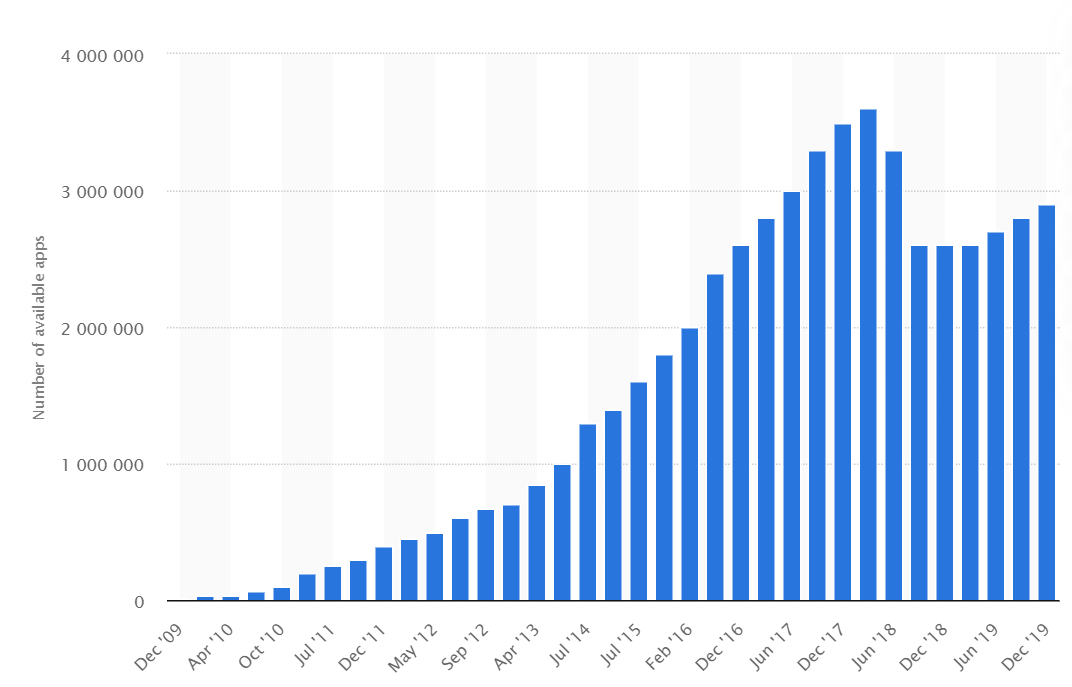
\includegraphics[width=0.9\textwidth]{./Figures/edwin-intro-app-number.png}
	\caption{Google Play 应用商店架上应用总数变化趋势}
	\label{fig:app_number}
\end{figure}

随着Android移动应用行业快速发展,移动黑灰产\footnote{即移动端黑色产业与灰色产业,下文同}也逐渐活跃。
黑灰产是以侵害用户、原应用作者或其他第三方利益为手段,凭此或通过其他可疑方式牟利的产业。
一方面,随着开发移动应用的门槛逐渐下降,开发一个移动应用的成本已经普遍低于开发一个类似的桌面级应用所需的成本~\cite{wasserman2010software};
另一方面,移动应用功能在实现上的灵活性~\cite{storydroid}增加了移动应用的复杂度,针对黑灰产的分析与拦截面临着多重新挑战。
两方面结合,为黑灰色应用进入移动端发展提供了良好的基础。

仿冒应用就是一类广泛存在的移动灰黑产产物。
本文研究的仿冒应用指代开发者根据市面上热门应用的外观仿制的Android应用。
据日常观察,仿冒应用中常有恶意广告弹窗、信息窃取、恶意扣费等行为,开发者可在用户使用仿冒应用时利用广告流量或非法获得的用户信息获利。
一方面,仿冒应用损害了原版应用开发者的知识产权,侵害了原开发者的利益;
另一方面,仿冒应用中的恶意行为也在威胁普通用户的信息安全。
可以联想如下场景:用户尝试通过应用市场搜索安装一个应用,应用市场返回了多个无论是名字或是图标都十分相像的结果,在未有明确指引的情况下,用户安装了仿冒应用。
前人针对Android恶意应用的研究~\cite{Zhou2012DissectingAM}显示,恶意行为可被自动触发,若用户下载的仿冒应用中包含此类恶意行为,用户数据安全将受到损害;
同时,由于用户不能分辨原版应用与仿冒应用,后者的不良用户体验会导致用户对前者乃至应用市场产生不良评价;
即使用户删除仿冒应用、装上原版应用,也浪费了时间和人力成本。

综上所述,仿冒应用影响用户搜索与下载应用时的安全和体验,最终使用户、原版应用开发者和应用市场三方利益均受到损害。
为了消除仿冒应用带来的隐患,无论是开发者、应用市场或是普通用户,都应对仿冒应用的特征与行为有所了解。

\section{研究现状}
尽管客观上存在对仿冒应用进行了解的需求,本研究对移动应用领域的前期调研显示,针对仿冒应用进行的实证研究尚缺乏,也未有公开可用的仿冒应用数据集。
因此,本节讨论与仿冒应用同属于移动灰黑产的重打包应用和恶意应用、以及其他移动应用领域相关方向的研究现状。

\subsection{重打包应用的研究现状}
\label{sec:repackaging}
重打包指恶意开发者对原应用解包、篡改内容之后再将应用重新打包的技术~\cite{khanmohammadi2019empirical}。
重打包应用侵害了应用原作者的知识产权,甚至可能具有恶意行为,因此也属于移动黑灰产范畴。
目前针对重打包应用的相关工作分为三类,分别为关于重打包的实证研究、针对重打包应用的检测和防止应用被重打包的研究。

相关实证研究方面,Khanmohammadi等人对重打包应用进行了一次详尽的实证研究~\cite{khanmohammadi2019empirical}。
该实证研究利用已有数据集AndroZoo~\cite{li2017androzoo++},得出了``重打包应用的主要目的为利用广告获得收入''的结论,并回答了包括``何种类型的应用会被重打包''、``重打包对原应用属性更改如何''在内的五个研究问题,增进了研究者对重打包应用的理解。


在重打包应用检测方面,早期工作通过比对两两应用之间的信息获得应用之间的相似度。
有研究者基于应用指令序列的方法使用模糊哈希的方法提取出应用的摘要信息,如DroidMOSS和DroidAnalytics~\cite{DroidMOSS, Zheng2013DroidAnalyticsA};
也有使用静态数据依赖构建程序依赖图(Program Dependency Graph, PDG)比对应用的方法,如DNADroid~\cite{DNADroid}和AnDarwin~\cite{AnDarwin},Centroid~\cite{Centroid}甚至为应用中的每个函数构建了三维控制流图(3-Dimensional Control Flow Graph, 3D-CFG),将三维控制流图聚合后,通过检测不同应用在控制图聚合后的质心位置判断应用间的相似程度;
还有算法通过比对抽象语义树检测重打包应用,如Hanna等人的Juxtapp~\cite{hanna2012juxtapp}利用K-gram模型对应用的二进制操作码序列进行比对,CLANdroid~\cite{CLANdroid}通过分析五种语义特征点(比如代码中的标识符和调用到的Android API等),以检测相似应用。
上述算法一来因为需要使用静态分析方法对代码进行解析,在遇到使用过代码混淆处理(如反射和代码加密)的应用时性能往往较差;二来需要基于两两比对进行检测,复杂度较高,在应用规模增大时会导致庞大的计算量。
为处理静态分析带来的问题,有学者提出了利用动态分析比对应用的方法,如Wu等人使用HTTP流量对应用行为进行建模~\cite{wu2015detect}。
亦有研究使用信息可视化方法检测重打包应用:ViewDroid~\cite{ViewDroid}通过重建和比对应用的视图筛出重打包应用,DroidEagle~\cite{sun2015droideagle}则利用UI布局相似性检测,Kywe等人比对应用中的文本与图像相似性以寻找相似应用~\cite{kywe2014detecting},Soh等人分析应用运行时收集的UI信息以检测重打包行为~\cite{soh2015detecting}。
而从避免两两比对、减小算法复杂度方面考虑,有学者提出利用第三方库进行检测的办法,如CodeMatch~\cite{CodeMatch}筛选出应用中使用的第三方库代码后,计算并比对剩余部分代码的哈希值,获取不同应用的相似程度;Wukong~\cite{Wukong}也分两步检测重打包应用,但与CodeMatch相比,其第二步使用了基于计数的代码克隆检测手段,而非基于哈希的技术。

防止应用被重打包的研究多基于检测原有代码是否被更改而开展。
Zhou等人提出了两个基于改版Dalvik虚拟机的对抗工具:其中,AppInk~\cite{zhou2013appink}利用一种``水印''技术(Watermarking)对抗重打包,但需要利用一个改版的Dalvik虚拟机进行文件检查;另一工具DIVILAR~\cite{zhou2014divilar}为应用的Dalvik代码提出了一种新编码形式,同时也需要修改用户设备Android系统中的Dalvik虚拟机以对新的编码进行解码。
Luo等人提出了在代码中注入大量检测节点的方法对抗重打包,并推荐开发者进行代码混淆,以避免令重打包开发者发现注入的检测节点~\cite{luo2016repackage}。
与之相似,Zeng等人也提出了在代码中注入逻辑炸弹的方法,并在研究中讨论了多种避免重打包开发者发现代码注入的策略~\cite{zeng2018resilient}。

\subsection{恶意应用的研究现状}
针对恶意应用的研究可分为两个方面,分别是面向恶意应用进行实证研究工作与面向恶意应用检测的研究。

面向恶意应用的实证研究众多,较有代表性的有以下两篇文献:
Felt等人的研究~\cite{Felt2011ASO}仔细剖析了来自多个不同平台的46个恶意程序样本以了解这些样本的激励机制,揭示了这些样本的运行机制和行为策略,为后人抵御此类恶意行为提供参考;
Zhou和Jiang~\cite{Zhou2012DissectingAM}搜集了来自多个主要恶意应用家族的、超过1,200个恶意应用样本,并系统性地描绘了这批样本的不同性质,包括其安装手段、激活机制和其如何执行有效负载(实现恶意行为)。
虽然恶意应用与仿冒应用有重合之处,但两者有一定区别,相关理论知识直接套用并不合适。

以上述实证研究与数据分析作为基础,研究者对恶意应用有了较好的了解,从而得以有针对性地进行恶意应用检测。
相关方法可大致分为静态分析、动态分析与机器学习三个方向。
早期研究通过静态分析手段对恶意应用进行检测,包括Enck等人提出的Kirin,在应用安装时检测应用权限,从而拦截恶意应用的安装~\cite{enck2009lightweight};
Felt等人提出的Stowaway~\cite{felt2011android}利用API调用分析和权限分析,寻找权限过大(Overprivileged)的应用;
RiskRanker~\cite{grace2012riskranker}则提出了一个两阶恶意应用检测手段,先筛选出具有root行为和可能导致隐私泄露的应用,再找出其中具有危险Dalvik代码加载行为的应用。
然而,受静态分析方法本身的限制,此类研究在遇到代码混淆时多被影响性能。
因此,有研究者利用动态分析技术对恶意应用进行检测。
TaintDroid~\cite{enck2014taintdroid}和DroidScope~\cite{yan2012droidscope}均在沙箱中对应用行为进行监视,TaintDroid利用污点分析技术寻找应用的信息泄露行为,DroidScope则从Android系统的不同层面分析应用的可疑行为。
Zhou等人\cite{zhou2012hey}提出了DroidRanger,利用应用行为比对与动态加载分析的方式,成功地从5个应用市场的204,040个应用中找出了211个恶意应用。
ParanoidAndroid~\cite{portokalidis2010paranoid}提出了将恶意检测方法迁移到云端的概念,将设备上的所有操作同步到云端服务器,从而在不影响设备本地功能的情况下进行恶意行为检测。
无论是静态分析方法或是动态分析方法,都需要人工对恶意行为的模式进行描绘,而用人工手段提取行为模式,不仅对领域知识有较高要求,还往往是费力费时的。
针对此问题,研究者开始利用机器学习技术检测恶意应用。
Chen等人从大规模数据集中总结出了恶意应用的两类特征,再将其用于分类器模型训练,提出了检测工具StormDroid~\cite{chen2016stormdroid},与之类似的方法还有CrowDroid~\cite{burguera2011crowdroid},DroidMat~\cite{wu2012droidmat},Adagio~\cite{gascon2013structural},MAST~\cite{chakradeo2013mast},DroidAPIMiner~\cite{aafer2013droidapiminer}与Drebin~\cite{arp2014drebin}。

\subsection{其他相关研究}
Andow等人针对灰色应用的研究~\cite{Andow2016ASO}从Google Play应用商店中采集了多个应用样本。
该研究将样本分类,定义了高仿应用(Imposter)、移动广告应用(Madware)等9种不同的灰色应用。
灰色应用指不具有明显恶意行为,但应用意图存疑、又或是会向系统申请过多权限的应用程序。
因此,这类应用不是恶意应用,但由于其盈利方式可疑,可将其归入移动黑灰产内。

另一方面,Hu等人针对市面上的欺诈约会应用进行了一次实证研究~\cite{hu2019dating}。
该研究中的欺诈约会应用声称自己为约会应用,实则诱导用户开通会员服务,也应归入黑灰产应用范畴。
分析发现,用户在此类应用中遇到的其他``用户''多数不由真人控制,而是具有预设对话模板的聊天机器人。
此外,研究还分析了该类应用的商业模式与分发渠道,评估了受害者的数量,对此类应用的生态进行了详尽解读。
该研究还通过直接检测相同评论和标记可疑用户的方式对此类应用进行排名欺诈检测。

Chen等人发布了漏洞检测工具Ausera~\cite{chen2018ausera},该工具通过静态分析技术与敏感词识别,对手机银行应用进行自动化三段式风险评估。
同期,他们在一个实证研究中利用Ausera从693个手机银行应用中检出超过两千个漏洞,向对应的60家银行发送了漏洞报告,并检查了新发行的手机银行应用以跟进漏洞修补进程~\cite{chen2018mobile}。
在被检出漏洞的60家银行中,21家确认了该研究反馈的漏洞,进行了对应修复,作者随后根据修复状况进行案例研究,分别面向银行、学者与政府,共给出了9条用于改善手机银行应用安全性与市场环境的实用建议。
与之类似,本研究也从多个方面出发,提出了防范仿冒应用、净化市场环境的实用建议。

% \subsection{针对应用评论的相关研究现状}
% 近年来,除了利用应用程序牟利以外,移动黑灰产业也开始进入应用市场评论的领域。
% 相关工作也可以分为检测与相关的实证研究两类。

% 检测方面,
% Zhu等人提出了一个利用评价历史记录检测应用是否具有排名欺诈行为的研究~\cite{zhu2014discovery}。
% 该研究提出,一般应用的排名在上升期(Raising phrase)和下降期(Recession phrase)之间会有一段维持期(Maintaining phrase),维持期过短且排名在短时间内剧烈波动的应用很可能具有排名欺诈行为。
% 然而,用该方法进行检测需要持续收集应用在市场上的评分数据,因此对数据采集有一定要求。
% Lim等人分析了差评水军(Review spammers)的特征并将其用于建模,以检测类似行为~\cite{lim2010detecting};
% Xie等人利用图论挖掘评论中开展共谋攻击(Collusion attack)的用户群组~\cite{xie2014grouptie},并在后续研究中将该方法拓展成一个检测系统~\cite{xie2016you}。
% 与之相似,Chen等人同样使用了基于图论的方法检测共谋攻击~\cite{chen2017toward},
% Hooi等人的FRAUDAR通过寻找二分图中的密集子图寻找关系特别密切的用户与应用,从而找出可能提供排名欺诈服务的可疑用户与使用了该服务的应用~\cite{hooi2016fraudar}。

% 实证研究方面,Rahman等人对Google Play中虚假评论行为的实证研究~\cite{rahman2019art}在公开确认该产业链存在的同时,也揭露了该产业的行为模式、生存情况甚至从业人员收入水平等方面的信息。

% 作为黑灰色产业链下游环节,虚假应用评论(即排名欺诈行为)已在前述研究中被证明与欺诈约会应用存在关联。
% 因此,排名欺诈也很可能与仿冒应用相结合,为移动黑灰产从业者牟取更多利益,有必要开展相关分析进行确认。

\subsection{研究现状小结}
综合上述分析,与仿冒应用同属黑灰产的重打包应用和恶意应用,甚至是日常生活中常用的手机银行类应用,均有对应研究可提供参考。
前人的实证研究收集了较为大量的重打包应用、恶意应用和手机银行应用数据,并提供了重打包应用与原版差异、恶意应用传播方式与负载执行方式、手机银行应用常见漏洞等指导性信息,帮助专业人员改善现有移动应用环境。
在丰富的前序研究提供的领域知识与数据支持下,各界才得以对重打包应用、恶意应用开展后续的检测研究。
相比之下,仿冒应用的相关数据和研究成果都乏善可陈。

换言之,在上述研究中,无论是对恶意应用还是重打包应用进行检测,都需要有一定领域知识或洞见(Insight)作为理论支撑。
对仿冒应用而言,学术界与工业界对其认知均较贫乏,``基于新见解进行技术拓展改良''式的研究手段尚未适用于仿冒应用。
因此,着眼于领域知识梳理的实证研究更适用于仿冒应用在当下的研究场景。
% \subsection{实证研究}
% 实证研究是一种基本研究技术,旨在针对特定方法在实际应用场景下的真实状况或对应产物进行数据收集、调查与分析,以让研究者了解事物的工作原理或使理论得以验证。
%
% 在软件工程领域,由于理论研究与工程实践结合较为紧密,学者采用需要检验理论在实践中的落地情况(如程序语言提供的特性是否被良好地理解与使用~\cite{bieman1995reuse}、是否在工程实践中体现优势等~\cite{harrison2000experimental}问题)或是调研现实应用场景中产生的现象(如恶意应用、重打包应用等在移动端市场出现的实际问题~\cite{Felt2011ASO, Zhou2012DissectingAM, Andow2016ASO, wang2018android}),实证研究技术是十分适合的方法。
% 因此,有越来越多的研究者使用实证研究技术对研究主体进行探索\cite{Felt2011ASO, Zhou2012DissectingAM, Andow2016ASO, wang2018android, chen2018ausera, chen2018mobile, bieman1995reuse, harrison2000experimental, dybaa2008empirical, manotas2016empirical, mcintosh2016empirical, mcilroy2016fresh, wu2016ji, yang2015xin, hu2019dating, khanmohammadi2019empirical}。
% 随着实证研究技术在软件工程领域中的认可度逐渐提高,软件工程顶级会议FSE与ICSE近年分别新设立了面向工业界的投稿分区,鼓励学者多基于应用场景进行实证研究,探明业界现状。
%
% 为向软件工程领域进行实证研究的学者提供方法论支持,Kitchenham等人基于自身在评阅软件工程项目的经验和一份针对医学研究者的研究指引,总结出了一份对于软件工程实证研究的初步准则(Preliminary guideline)~\cite{kitchenham2002preliminary},对实证研究的数据收集方法、实验设置方法等各个步骤都给出了严格指引,如在数据收集时需要确保数据的准确性与完整性,需要保证实验的可重复性等。
% 为保证数据的准确性与完整性,本研究利用\mytool 尽可能全面地收集多个来源的应用样本。
% Seaman则结合实例,提供定性分析的~\cite{seaman1999qualitative}。
% 在实证研究可采取的具体方式方面,Easterbrook等人于2008年提出了面向软件工程领域的实证研究方法建议~\cite{easterbrook2008selecting},为软工实证研究提供方法论参考,文中将实证研究方法论分为受控实验、案例分析、调查研究、社会学意义研究与混合方法途径等多类,以适用于不同场景。
% 本研究采取了其中的案例分析方法。
%
% 前期调研显示,针对仿冒应用进行的实证研究尚缺乏,也没有公开可用的仿冒应用数据集。

\section{拟采用的研究方法}
上述研究现状说明,实证研究在多个研究方向上提供了研究数据或领域知识,有一定实用价值。
当下的仿冒应用研究,既缺乏可用的数据集,也缺乏对应的基本特征知识。
作为基于数据采集和数据分析的技术,实证研究方法正好可缓解仿冒应用领域知识和数据集的缺失,是适用于本课题的技术手段。
本研究将采用实证研究方法,对仿冒应用进行研究。

实证研究是一种基本研究技术,旨在针对特定方法在实际应用场景下的真实状况或对应产物进行数据收集、调查与分析,以让研究者了解事物的工作原理或使理论得以验证,其中数据收集是十分重要的一部分。
前人总结~\cite{kitchenham2002preliminary}对实证研究的数据收集方法给出了严格指引,指出数据收集时需要确保数据的准确性与全面性。
因此,科学地进行数据收集是本研究面临的一个关键问题。

% \section{问题分析与研究难点}
% 前文的研究现状,反映出移动应用领域是目前的研究热点之一,也反映出移动黑灰产无孔不入的特点。
% 为了保障正当开发者的利益与消费者的权益,学术界和工业界都需要对移动黑灰产有更全面、更深入的理解,从而更好地预防未知的威胁。
% 上述研究现状表明,工业界与学术界的软件工程、安全领域在移动应用的研究上已经取得了丰富的成果。
% 然而,现有研究提供的知识仍有空缺部分,移动黑灰产的仿冒应用部分正是缺口之一。
% 在仿冒应用相关研究缺失的情况下,仿冒应用数据严重匮乏,造成了以下问题:
%
% 1)\	\emph{无法对仿冒应用进行定量分析} \quad
% 目前,学术界与工业界目前对恶意应用和排名欺诈行为均有良好理解,厂家得以在实践中抵御、规避此类移动黑灰产的侵袭,这得益于前人在实证调查研究~\cite{Felt2011ASO, Zhou2012DissectingAM, zhou2012hey, rahman2019art}中提供的数据与洞见(Insight)。
% 然而,在仿冒应用数据缺失的情况下,相关定量分析与定性分析无法进行,无法让学术界与工业界对仿冒应用有清楚了解。
% 针对仿冒应用进行实证研究可以有效解决这个问题。
% 具体而言,研究者可从工业界环境(即各应用市场)中获取大量应用,从所获应用中筛选出一定数量的仿冒应用,提取出其中可用于定量分析的数据,从而开展相关分析。
%
% 2)\	\emph{无法确定仿冒应用的性质} \quad
% 尽管仿冒应用在日常生活中随处可见,却少有研究者对其进行研究。
% 因而,仿冒应用的形态尚未明确,亦从未有前人评估仿冒应用的风险性;总结仿冒应用的发展趋势不明,无法确定这一移动黑灰产是否会更加壮大;仿冒应用的市场反馈无人探索,仿冒应用是否会与其他黑灰产业环节结合更是不得而知。
% 针对以上疑问,研究者可采用实证研究的混合方法途径方法论可以通过对数据定性分析,帮助理解仿冒应用具有的性质;而相对的案例分析(Case studies)方法论~\cite{easterbrook2008selecting}则可以在案例支持下更有力地确认定性分析的发现。
%
% 综上,现时仿冒应用数据匮乏、对仿冒应用了解缺失的问题,可通过实证研究缓解。
% 因此,本文与犇众信息的移动安全威胁数据平台Janus~\cite{janus}合作,搜集并分析了大量应用样本,从仿冒应用特征解读和仿冒应用评论分析两方面进行了大规模实证研究,对仿冒应用作出了较为全面的剖析,填补了本领域的研究空白。
% 仿冒应用特征解读利用数据挖掘分析技巧,利用本研究收集到的仿冒应用数据对仿冒应用进行画像,为多方受众提供可借鉴的结论;
% 仿冒应用评论分析则通过收集仿冒应用在市场上获得的反馈,验证仿冒应用和排名欺诈行为的关系,进一步地提供了关于仿冒应用生态的信息。
%
% 在实证研究中,研究者通常都会遇到几点挑战:如何确定研究主体、如何收集数据、如何对数据进行有效处理;
% 而在排名欺诈相关研究中,如何从评论数据中有效挖掘排名欺诈行为是研究者经常要思考的问题。
% 故本实证研究中的难点可概括如下:
%
% 1)\	\emph{如何确定仿冒应用} \quad
% 仿冒应用和正版应用是相对的概念。
% 本文选择了市面上最热门的50个应用,再搜集其对应的仿冒应用样本。
% 从应用中筛选出与热门应用外观相似或是相同的样本后,本文使用Android本身自带的证书机制,将获得样本的证书信息与原版应用的证书信息进行比对,从而鉴别出仿冒的样本。
%
% 2)\	\emph{如何获得针对仿冒应用的大量数据} \quad
% 数据搜集是科研工作中公认的难点。
% 本文想要提供一次全面的研究结果,除了搜集的目标应用需要有多样性之外,也必须获得不同应用市场上的数据,增加研究的代表性。
% 前文提及犇众信息的移动安全威胁数据平台Janus是一个数据整合平台。该平台每天从各大Android应用市场爬取应用样本入库,免去了要针对各个市场重新定制爬虫代码的麻烦。
% 通过设计和实现仿冒应用收集框架\mytool,本文顺利从Janus搜寻到了近14万条数据条目作为原始数据,其中每条数据条目代表Janus从应用市场上获得的一个应用样本。
%
% 3)\	\emph{如何对大量的数据进行有效处理} \quad
% 数据规模和处理效率一直是一对矛盾。
% 由于一条数据条目代表一个应用样本,要对所有应用样本进行详尽分析,明显太耗费时间成本与计算成本;然而,如果只对样本进行简单处理,获得的分析结果就不够全面和深入。
% 在尽量确保分析全面性的前提下,对于每个样本,本研究只抽取8个关键信息项进行分析,以节省时间与计算成本。
%
% 4)\ \emph{如何挖掘评论中的排名欺诈行为} \quad
% 现有的排名欺诈挖掘工作均具有其各自的局限性,或是对评分数据有连续收集要求,或是要求检测者有已知的排名欺诈群体,并不能直接应用到本研究收集的数据中。
% 为此,本研究先后设计了基于用户行为可信度和基于评论内容重复度的两个方法。
% 前者规避了现有方法的局限性,后者进一步解决了大数据量带来的大运算量问题。

\section{本文拟解决的关键问题}
上一节提及,科学地进行数据收集是本研究面临的一个关键问题。
此外,本研究还有两个关键问题,一并列举如下:

\begin{itemize}
	\setlength{\itemsep}{1pt}
	      \setlength{\parskip}{0pt}
	      \setlength{\parsep}{0pt}
	\item \emph{如何科学地获取针对仿冒应用的数据?} \quad
	      由于仿冒应用数据缺失,本文只能自行收集数据。
	      数据搜集是科研工作中公认的难点,为提供一次全面的研究结果,除了数据需要有一定规模以外,搜集的目标应用也需要具备多样性,此外还必须获得不同应用市场上的数据,增加研究的代表性。
	      为此,如何获得大量真实、有效、全面而有代表性的数据将是本文研究的一个关键点。

	\item \emph{如何对仿冒应用进行理解?} \quad
	      仿冒应用虽然普遍存在于各大应用市场中,但尚未有研究对其进行分析,无论是应用市场、研究者还是用户,都缺乏对仿冒应用的理解。
	      为能较全面地认识仿冒应用,需要从不同角度对其进行解读。
	      因此,从应用基本属性、应用作者行为等多角度对仿冒应用进行解析,是本文研究的重点之一。

	\item \emph{是否能有效地筛选仿冒应用} \quad
	      根据日常经验不难发现,在现阶段,用户在实际使用中经常能搜索到仿冒应用,应用市场对仿冒应用的筛选排除并未完善。
	      恶意应用、重打包应用的研究发展表明,充分认识移动黑灰产应用特征对后续的对应检测、发现有明显促进作用。
	      同理,作者希望可基于对仿冒应用进行的解读与画像,设计有效流程帮助各大市场梳理、排除仿冒应用。
	      这是本文研究的另一重点,也是本文的创新点。
\end{itemize}

\section{本文主要工作}
为解决上述三个关键问题,本研究完成了如下主要工作:

\begin{itemize}
	\setlength{\itemsep}{1pt}
	      \setlength{\parskip}{0pt}
	      \setlength{\parsep}{0pt}
	\item \emph{全面的数据集整理} \quad
	      借助自行实现的仿冒应用收集框架,本研究尽可能全面地收集了来自29个应用来源的约14万个应用样本,并从中筛选出5万个仿冒样本,整理成已知的首个仿冒应用数据集,以供其后的相关研究使用。

	\item \emph{仿冒应用数据画像与现实案例分析} \quad
	      本文从基本信息与开发者行为两个方向入手分别进行了实证研究,前者对仿冒引用进行了较为全面的数据画像,后者根据仿冒应用开发者行为推断出现有应用市场监管不足之处。
	      两组研究除了从较高维度进行数据分析外,还从数据集中挑选出应用和证书实例,分别展开案例讨论,以深化在数据画像和行为分析中得到的领域知识。

	\item \emph{提供实用建议} \quad
	      基于在实证研究中的发现,本文分析了仿冒应用特征的可能成因与现有应用市场的不足之处,由此分别面向普通用户、应用市场和相关从业者提供了实用建议。

	\item \emph{基于规则的仿冒应用检测框架} \quad
	      依靠前序研究中对仿冒应用的理解与解读,作者设计并实现了基于规则的仿冒应用检测框架\mytool 。

\end{itemize}

% 现有的排名欺诈挖掘工作均具有其各自的局限性,或是对评分数据有连续收集要求,或是要求检测者有已知的排名欺诈群体,并不能直接应用到本研究收集的数据中。
% 为此,本研究先后设计了基于用户行为可信度和基于评论内容重复度的两个方法。
% 前者规避了现有方法的局限性,后者进一步解决了大数据量带来的大运算量问题。

% \section{研究方法与工作概览}
%
% \subsection{研究方法}
% 前文已经提及,实证研究能够为研究主体提供画像与洞见,从而为对应方面的后续实践与研究提供建议与便利。
% 在软件工程领域与安全领域,已有多篇实证研究~\cite{Felt2011ASO, Zhou2012DissectingAM, Andow2016ASO, wang2018android, chen2018ausera, chen2018mobile, bieman1995reuse, harrison2000experimental, dybaa2008empirical, manotas2016empirical, mcintosh2016empirical, mcilroy2016fresh, wu2016ji, yang2015xin, hu2019dating, khanmohammadi2019empirical}为实践工作提供知识支持。
% 因此,本文亦将采用实证研究方式,对仿冒应用进行探索。
%
% 与相关文献~\cite{easterbrook2008selecting}提供的方法结合,本文研究中使用到的是案例分析方法。
% % 1)\ \emph{混合方法途径(Mixed-method approaches)} \quad
% % 混合方法途径指结合定量分析与定性分析,对研究对象进行系统数据解读的实证研究方法。
% % 按照实施的方式,混合方法途径可分为顺序解释策略(Sequential explanatory strategy)、顺序探索策略(Sequential exploratory strategy)与并发三角策略(Concurrent triangular strategy)三类。
% % 顺序解释策略先收集与分析定量数据,再收集和分析定性数据,以定性数据结果帮助解释定量结果;与之相反,顺序探索策略先收集与分析定性数据,再收集和分析定量数据,以定量数据结果帮助解释定性结果;并发三角策略则会同时采用不同方法,以试图确认、交叉验证或证实已有发现。
% % 本文的特征解读部分先采用定量分析方法分析数据,再采用案例分析方法给出定性结果,使用了顺序解释策略;而后续的仿冒应用与排名欺诈关联验证先给出定性结论,再提供定量数据支持,则使用了顺序探索策略。
% % \emph{案例分析(Case studies)} \quad
% 案例分析是软件工程领域最常用的实证研究方法,完整的案例分析通过确立研究问题、选择研究案例和收集数据三步研究真实场景中出现的现象,适用于真实环境为对研究主体产生影响的因素之一、又或是实验数据时间跨度较大的场景。
% 对于针对某些现象的初步调查,可使用探索性案例分析(Exploratory case studies)以提出新猜想和构建理论;而验证性案例分析(Confirmatory case studies)则用于验证现存理论。
% 本文的案例分析既包含用于提出新猜想的探索性案例分析,亦包含验证数据画像的验证性案例分析。
%
% \subsection{工作概览}
%
% \begin{figure}[htbp]
% 	\centering
% 	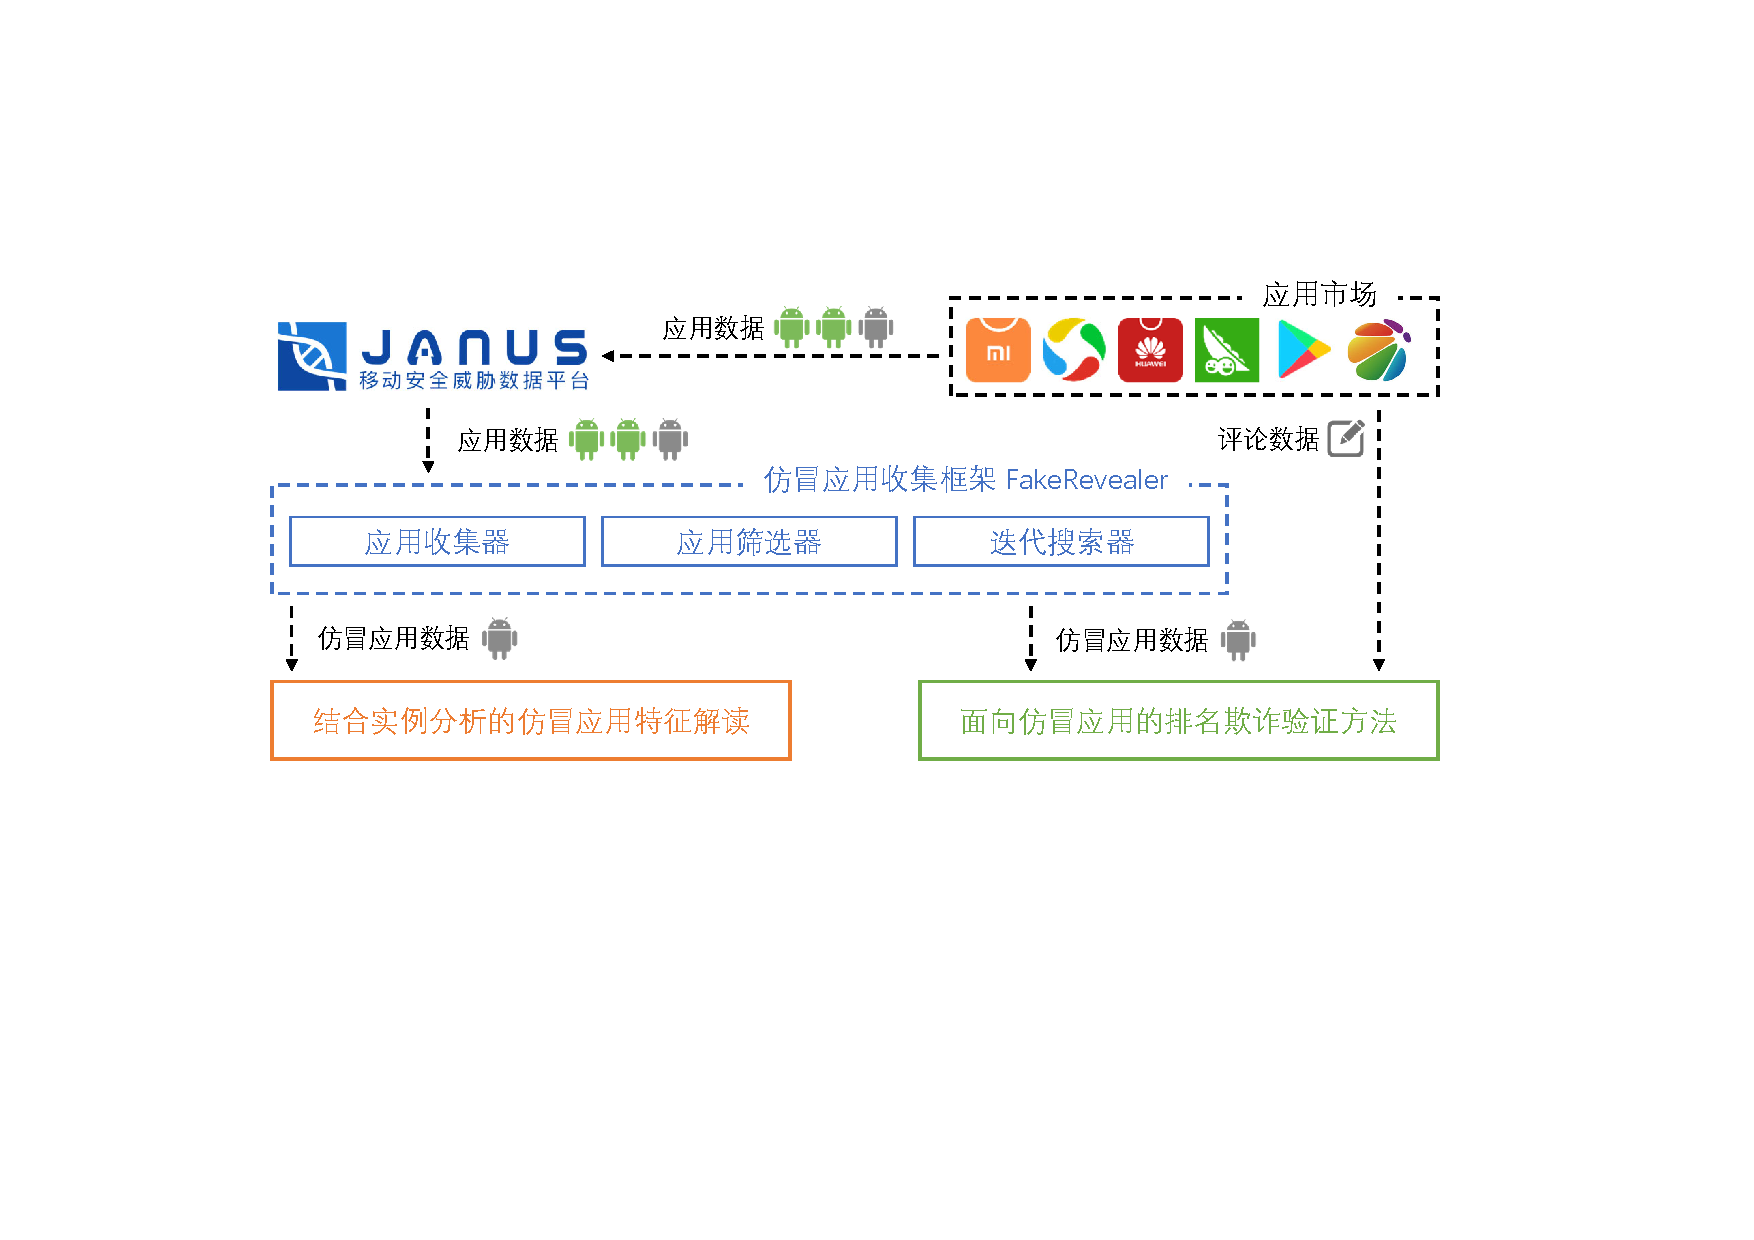
\includegraphics[width=\textwidth]{./Figures/edwin-overview}
% 	\caption{本文工作概览}
% 	\label{fig:Workflow}
% 	\vspace{-3mm}
% \end{figure}
%
% 本节为本文工作提供概览。如\autoref{fig:Workflow}所示,本工作通过三个主要部分,完成三部分工作:
%
% 1)\ \emph{利用面向仿冒应用的收集框架\mytool 收集大规模数据,解决仿冒应用数据稀缺的问题} \quad
% 针对实证研究中实验数据应尽可能具有完整性与代表性的要求,本研究设计并实现了仿冒应用收集框架\mytool,尽可能全面地进行仿冒应用的数据收集。
% 数据收集主要分为两个部分:正版应用信息的收集和仿冒应用的收集。
% 在正版应用信息收集的部分,本文选择了50个最热门的App作为目标应用,然后手动收集了跟这些App有关的信息;
% 基于该50款目标应用,本研究利用\mytool,收集了从29个应用来源获得的近14万个应用样本,并从中筛选出5万个仿冒应用,整理成集。
% 该数据集可为后续相关工作如代码分析、特征检测等提供数据支持。
%
% 2)\ \emph{首次针对仿冒应用的特性进行大规模的特征解读} \quad
% 针对移动黑灰产研究中关于仿冒应用的研究空白,本研究利用上述仿冒应用数据,结合案例分析,进行了首次基于Android系统仿冒应用的大规模特征解读。
% 特征解读从三个视角完成,这些视角分别是仿冒的基本应用特征、影响仿冒应用数量的因素和仿冒应用的发展轨迹,由浅入深揭示仿冒应用的生态。
% 对应的三个案例分析除了为特征解读提供案例支持之外,还揭示了更多仿冒应用开发者的行为特征,可为用户、应用市场和安全领域从业人员等多方受众提供一定见解。
%
% 3)\ \emph{面向仿冒应用的排名欺诈验证} \quad
% 该部分中,本文从第三方应用市场中随机选取一部分应用,爬取用户对它们的所有历史评价,以检测仿冒应用与排名欺诈行为的关联。
% 针对前人检测研究需要先验知识或特殊数据的问题,本研究从社交媒体研究引入了用户行为可信度进行排查,避开了现有方法的局限性。
% 进一步地,本研究从评论内容重复率方面提出了另一创新性排查方法,解决了数据量增大带来的大运算量问题。
% 人工复查结果显示,两种排查方法均取得了优于现有方法的结果。
\section{本文组织结构}
% todo: 7 chapters?
本文共分为七章,环绕着本研究的数据搜集和不同的分析方向展开,各章节内容如下:

\fullref{chp:intro} 主要提供了本文的研究背景、相关工作、本文拟采用的研究方法、拟解决的问题与本文的主要工作。

\fullref{chp:background} 介绍相关技术背景,从软件工程领域的实证研究出发,介绍实证研究的常用方法和数据收集、验证标准等理论背景,再着眼于本研究的主体——Android应用,介绍了Android安全证书机制和与仿冒应用相关的重打包技术。

\fullref{chp:research_settings} 介绍整个研究的设置,包括根据研究现状提出研究问题、确立研究对象,阐述数据收集的相关考量,并与其他研究收集的数据进行对比。

\fullref{chp:discoveries_basic} 从仿冒应用与原版应用相似度、影响应用被仿冒的严重程度的因素及仿冒应用行为三点入手,对与仿冒应用基本特征相关的三个方面进行实证研究,最后针对研究结果分别向用户、应用市场和应用开发者提供实用建议。

\fullref{chp:discoveries_behavior} 则结合应用证书视角与结合时间维度视角进行探索,分析现有应用市场监管策略存在的不足,针对性地提出改善措施。

\fullref{chp:framework_prototype} 提出了一个基于规则的仿冒应用检测框架,并将前两章实证研究所得的经验总结为规则,对框架进行了有效性检验。

% % 这些视角包括仿冒应用特征、影响仿冒应用数量的因素和仿冒应用的发展轨迹,每个视角都被进一步分解成多个不同的研究问题。
% % 说明仿冒应用的数据收集方式并详细介绍其中三个组件(\componentA、\componentB 和\componentC)的设计与实现,
% % 结束解读后,本文从数据中挑选三个具有代表性的案例进行分析,以案例进一步深化分析结果。

% \fullref{chp:feedback} 针对仿冒应用进行了排名欺诈检测。
% 针对现有检测方法的不足,本文先后提出两个具有创新性的方法对排名欺诈行为进行排查,并将排查结果与前一章的仿冒应用进行比对。
% % 结果显示,仿冒应用存在排名欺诈行为。仿冒应用与排名欺诈行为作为移动黑灰产的两个环节存在关联。

\fullref{chp:future} 对本文工作进行总结,并对下一步工作进行展望。

\clearPaperPage

\chapter{Android背景介绍}
\label{chp:background}

本章主要介绍Android系统、Android应用程序和应用市场相关的背景知识,包括现有的Google Play市场和多个第三方市场共存的局面介绍,同时也会介绍Android安全证书机制的相关背景。

\section{Android系统介绍}
Android系统是属于Google公司的开源操作系统,基于Linux内核研发。
其最早版本于2008年发布(Android 1.0),起先只针对手机端发布。
由于具有图形化操作界面,并且采用触屏作为交互方式,极其简单易用,Android系统自发布起就迅速在智能手机领域抢占大量市场份额,搭载Android系统的平板电脑也在我们的日常生活中渐渐变得随处可见。
近年来,随着IoT(Internet of Things,物联网)的发展,家用电器趋向智能化,不少电视厂商、机顶盒厂商、甚至可穿戴设备厂商也开始为产品内嵌深度定制的Android系统,为用户提供更好的体验。

\begin{figure}[htbp]
	\centering
	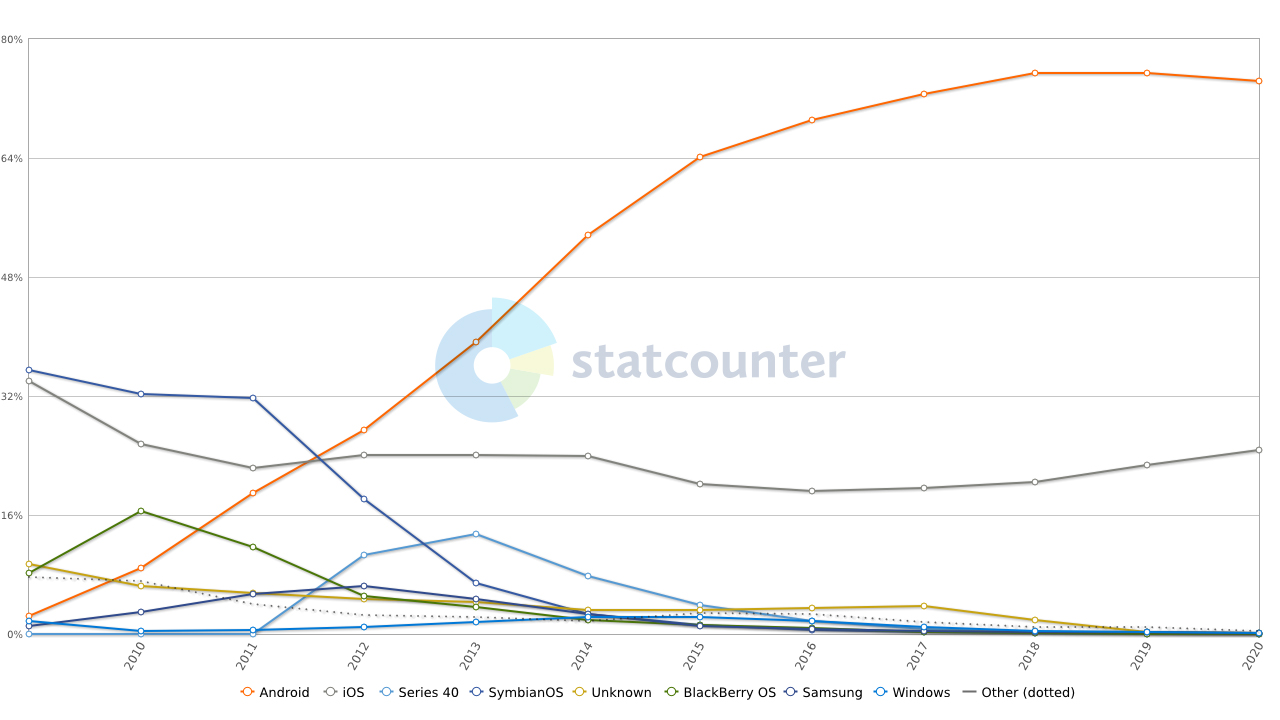
\includegraphics[width=0.95\textwidth]{./Figures/edwin-StatCounter-os-mkt-share-yearly-2009-2020.jpg}
	\caption{2009至2020年移动端操作系统市场份额变化图}
	\label{fig:Android-Mkt-Share}
	\vspace{-5mm}
\end{figure}

图~\ref{fig:Android-Mkt-Share}展现了2009年到2020年间不同移动端操作系统对市场占有率的变化曲线,图表来源于数据分析机构StatCounter~\cite{MobileOSMktShare},图表X轴为时间线,Y轴为市场份额占总量的百分比。
不同颜色的曲线代表不同操作系统,其中Android系统由橘红色曲线表示。
从图中数据可知,自发布以来,Android系统便一路高歌猛进,迅速占据移动端操作系统市场,从2012年起就获得了业界第一的市场份额占有率,直到2020年,其超过70\%的市场占有率依然遥遥领先于其他操作系统。
其中原因,除了对用户非常友好的操作方式以外,也在于其具有一个多元、开放又充满活力的应用程序生态环境。

\section{Android应用程序}

\subsection{应用程序简介}

Android应用程序(Android Application,简称App)是可以安装在Android系统上、拓展系统功能的软件,这些软件通常基于Java语言开发,其中可以包含用C语言或者C++编写的库以提高性能。
2014年起,Google宣布Android支持Kotlin编程语言,自此开发者也可以使用Kotlin语言进行Android App开发。

Android App的开发需要使用Google提供的软件开发工具包(Software Develop Kit,简称SDK)和Google支持的集成开发环境(Integrated Development Environment,简称IDE)。
SDK是包含了众多软件包的工具箱,其中有包括了Android系统应用程序接口(Application Programming Interface,简称API)的函数库和用以编译App的各种工具,在编译完成之后,开发者还可以利用SDK的相应工具为App签上自己的数字签名。
API函数库提供了Android系统的一系列接口,开发者需要在使用Android App框架的前提下,调用各种API实现自己设计的功能。

在发布每一版本Android系统的同时,Google公司也会发布一个新版本的Android SDK供开发者开发App。
每个人都可以从Android的官方网站上下载Android SDK和开发应用所需的IDE,这意味着,利用官方发布的工具,任何人都可以开发出属于自己的Android App。

\subsection{构建应用程序}

与大部分软件一样,开发者在发布自己的App之前,也先需要把代码编译打包成Android操作系统使用的一种应用程序包格式文件APK(Android application package)。
每个APK文件都会包含该款App的一系列基本信息,包括App的应用名、包名(Package name)、安全证书等。
其中,包名是Android系统识别App的依据,每款App在不同的版本可以有不同的应用名,但其包名必须是一致的。
图~\ref{fig:Android-Build-Process}展现了APK文件的构建流程。
一般来说,一个Android App的构建流程会分为以下四步,整个构建流程由Android SDK中的Android插件和Gradle构建工具管理。

\begin{figure}[htbp]
	\centering
	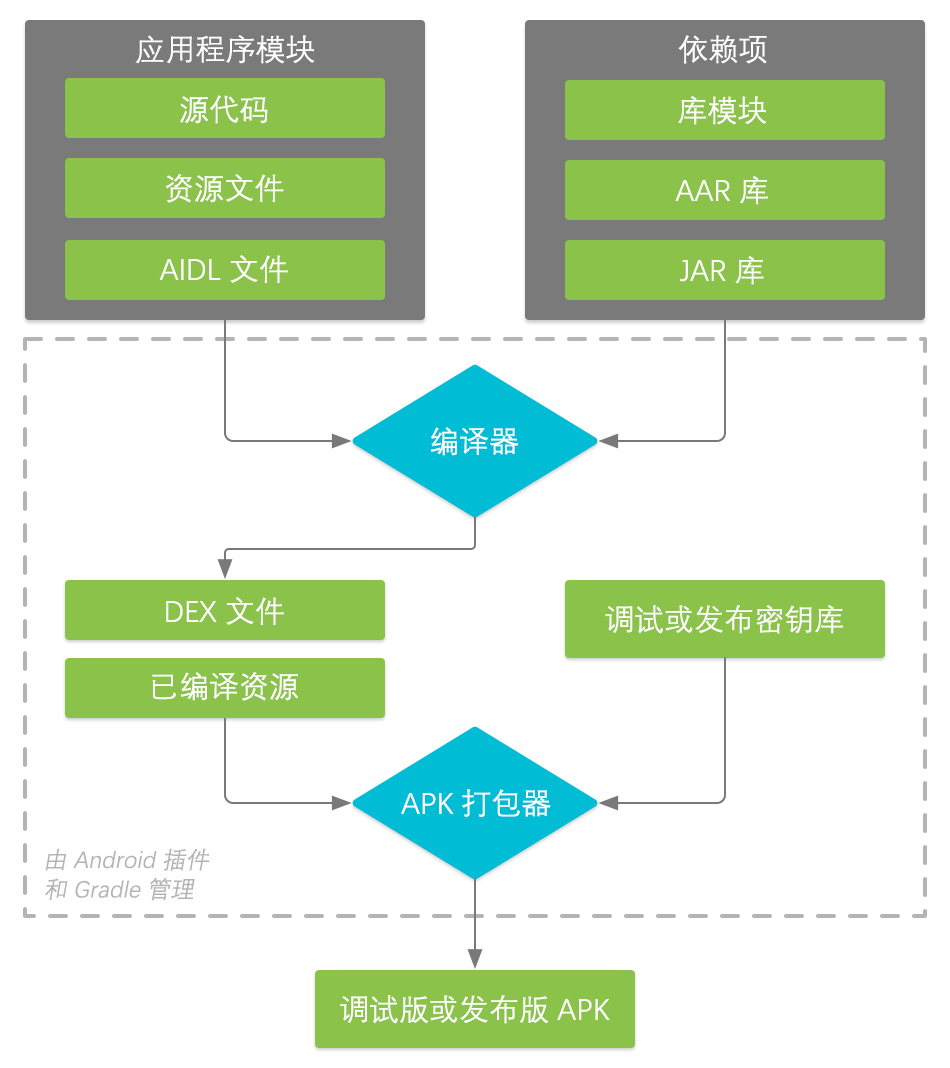
\includegraphics[width=0.6\textwidth]{./Figures/edwin-build-process-CHN.png}
	\caption{Android App构建流程}
	\label{fig:Android-Build-Process}
\end{figure}

首先,开发者需要编写App对应的源代码,然后连同一些源代码中使用到的依赖项一起输入到编译器中生成DEX文件。
源代码可以由Java语言或者Kotlin语言编写,而DEX文件则是一种可执行文件,可以运行于Dalvik虚拟机上。
Dalvik虚拟机则是Android系统的核心组成部分之一,用于运行被编译为DEX文件的程序。
此外,编译器还会将其他未被编译的资源文件转换为编译后的资源。

然后,SDK中的APK打包器会将DEX文件和已经编译好的资源文件一起打包。
APK文件的本质是压缩文件,其中包含了被编译的代码文件、App需要用到的资源文件(比如字符串、图片等资源)、assets资源、App的安全证书和Manifest配置文件,所以APK打包器的任务是将这些所有文件都压缩进一个APK文件里面。
不过,在这个步骤,APK打包器还未将所有文件压缩。
因为在压缩之前,还需要进行下一步的签名。

在第三步,APK打包器会使用密钥库文件对上一步中提及的资源文件和代码文件进行数字签名。
这个步骤是用作校验APK文件是否被篡改、保证APK文件完整性的一个重要步骤,在本章后续内容中会有相关机制的更多介绍。

最后,APK打包器会使用zipalign工具对应用进行优化,以减少App在设备上运行时所占用的内存。
这步结束之后,整个构建流程也随之结束。
开发者会获得一个编译好、签名完毕并且经过优化的APK压缩文件,然后就可以将这个APK文件安装到Android设备上运行使用。


\section{Android应用市场}
由于每个人都可以开发、构建自己的Android App,从网上发布的App数不胜数。这种开放性为Android应用生态带来开放性的同时,也会引入以下几个问题:

1)\ \emph{难以择优} \quad
开放的环境会导致App数量难以胜数。由于从互联网上找到的App质量良莠不齐,用户有时无法判断网上的应用是否符合自己的需求;

2)\ \emph{数据安全} \quad
智能手机与现代人的日常生活息息相关,其中也自然包含了各人的隐私数据甚至财产信息。确保用户下载、安装到的应用不会损害到他们的财产安全和数据安全至关重要;

3)\ \emph{宣传渠道} \quad
开发者希望自己的App尽可能地受欢迎,但中小开发者并没有足够的资源去宣传自己的应用,可能会导致原本质量优秀的App因为缺少宣传渠道而无人问津;

4)\ \emph{收入结算} \quad
开发者有从App中获得盈利的需求。即使是部分出于兴趣或其他非盈利目的开发手机应用的开发者,也需要从App中获取补贴以维持App的维护和正常运作。如何利用App变现、变现之后又要怎样将资金回流到开发者的问题有待解决;

5)\ \emph{应用更新} \quad
随着时间推进,用户的需求并非一成不变,开发者也需要针对App中以往出现的漏洞查漏补缺、或者更新软件功能,但要求用户定期/不定期地手动更新某个App甚至多个App并不现实。

Google发布的应用商店Google Play~\cite{GooglePlay}的存在缓解了以上的问题。它是Android操作系统的官方应用商店,可以让用户浏览和下载商店中的App。
一方面,普通用户可以经由Android系统中预装好的Google Play服务寻找、购买和下载心仪的App;另一方面,Google Play也允许开发者将App通过开发者账户上传到Google Play中,在经过一系列的审查之后上架到商场上供用户下载。与上述的五个问题对应,Google Play应用商店提供了以下几点服务:

1)\ \emph{一个由官方背书的下载渠道} \quad
这确保了用户下载的App得到官方认可。同时,Google Play也提供了一个关于App的社区条件,用户可以对App进行打分、评论,用户对App的评价经审核后可以由所有其他用户查看,直接影响其他用户对``是否要下载某款应用''的决定;

2)\ \emph{上架之前的应用审核} \quad
在开发者上传App时对App作出一定的审查,以排除部分恶意开发者在商场中上架病毒和恶意应用的可能性。Google Play也会根据用户反馈、应用本身运营数据等原因于每季度从商店中移除一部分App,以保证商店货架上App的质量;

3)\ \emph{作为激励机制的推荐榜单} \quad
在用户评价的基础上,Google Play筛选出一部分质量优异的App制订出一些推荐榜单。推荐榜单会在应用商店首页进行展示,榜单包括``编辑精选''、``热门应用''、``年度之选''等,其中既有大公司开发的App,也会有中小开发者独立开发的应用。此外,Google还会通过用户的使用习惯、所在地区等因素为用户提供个性化推荐(如图~\ref{fig:Google-Play-Main}所示),在不同的App类别下,也有不同榜单为用户推荐,加大了优秀App的曝光率;

\begin{figure}[htbp]
	\centering
	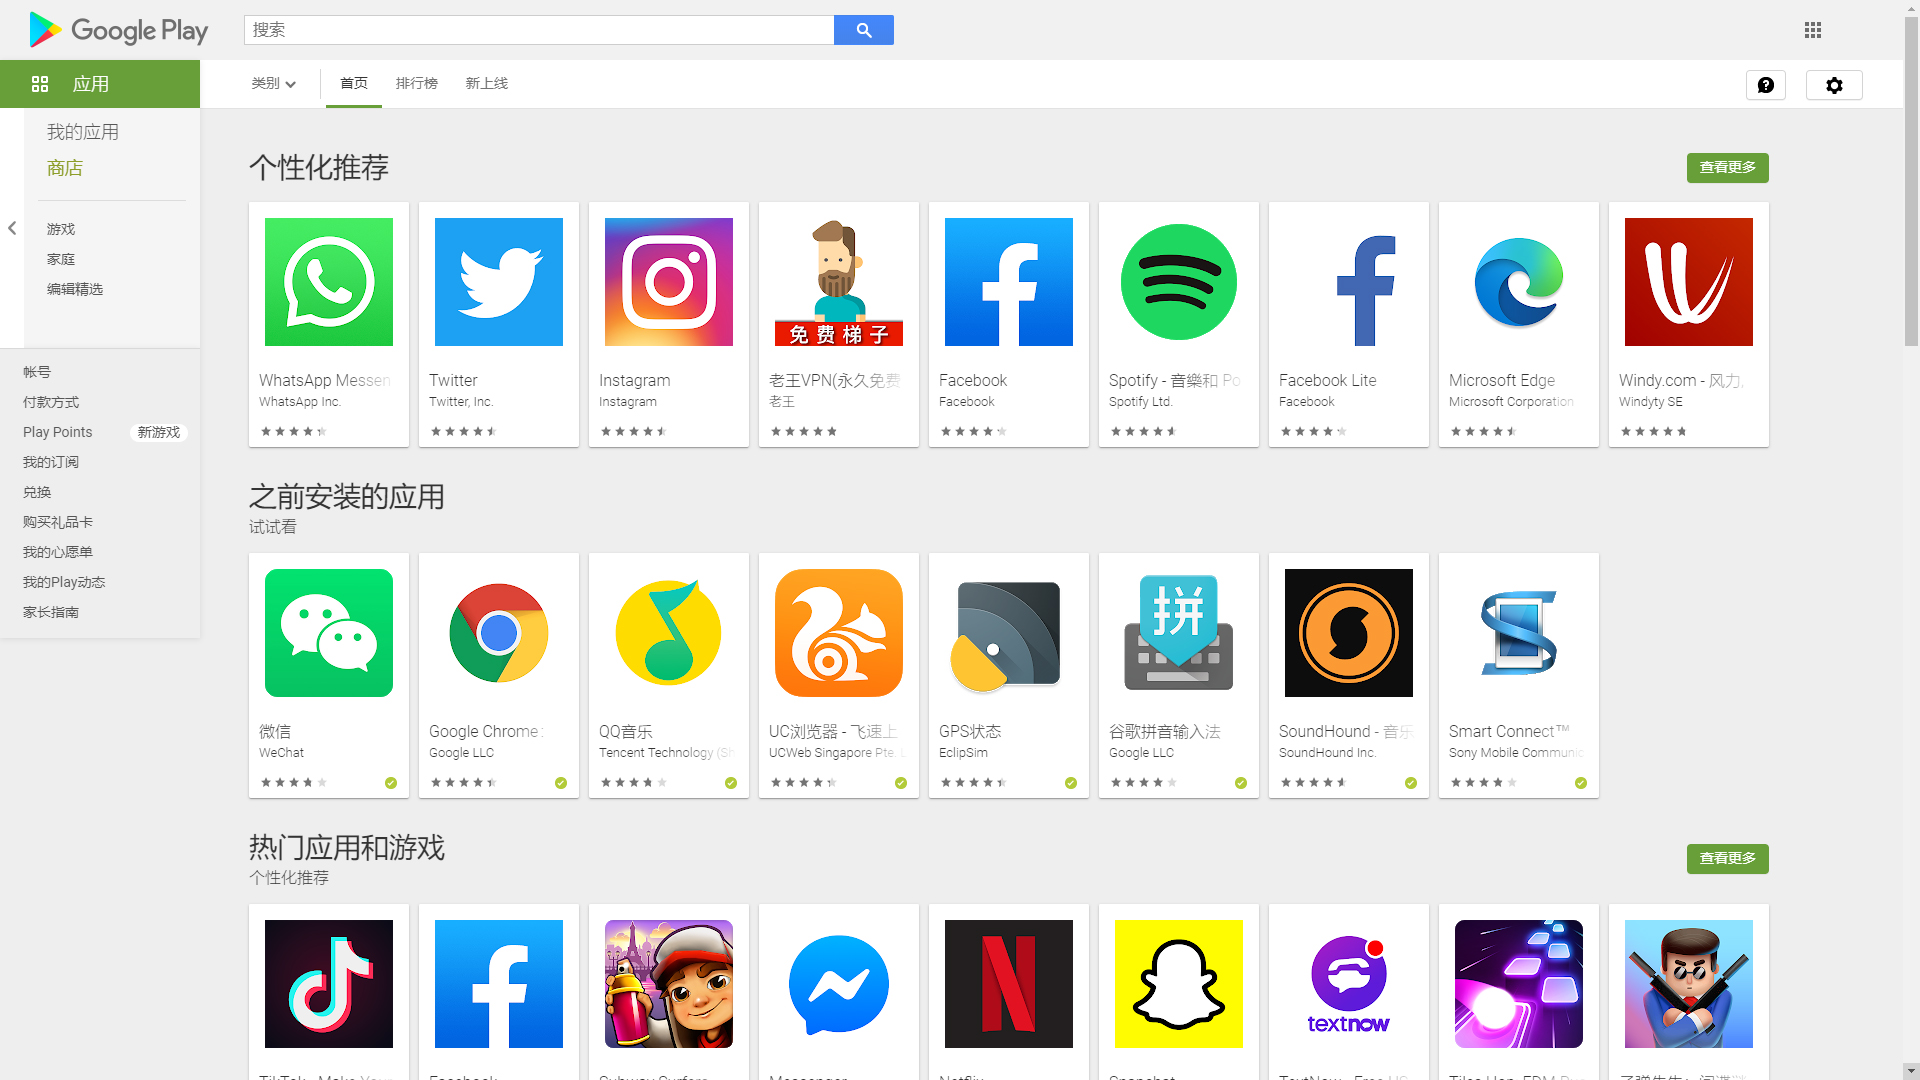
\includegraphics[width=\textwidth]{./Figures/edwin-google-play.jpg}
	\caption{Google Play应用商店首页(从桌面端浏览)}
	\label{fig:Google-Play-Main}
\end{figure}

4)\ \emph{集中的结算通道} \quad
Google Play应用商店为开发者提供了一个统一的结算渠道。应用开发者可以在App内销售商品,然后选择Google Play提供的集成结算服务。用户在购买服务时,直接向Google付款,Google再在每个结算周期将款项结算给开发者。这样一来,开发者尤其是独立开发者就可以更专注于App本身的开发,而不需要考虑如何利用应用变现、再将资金回收的复杂问题。Google Play也允许开发者将自己的App上架为付费应用,需要用户付款后才可下载;

5)\ \emph{方便快捷的更新推送} \quad
由于Google Play本身是个应用程序的集中平台,而且也预置到了大多搭载Android的设备中,所以开发者在更新应用时,只需将新版本上传到Google Play的后台,应用商店经过审核之后,就可以将新版本的应用推送到用户的设备中,让用户设备中的App实现自动更新,免去双方的麻烦。


\section{第三方应用市场}

Google Play应用商店无疑为用户和开发者都提供了一个优良的解决方案,每个应用底下由用户评论组成的社区也促成了用户和开发者之间的交流,用户反馈直接推动了开发者对应用的改良。

遗憾的是,由于种种原因,Google Play应用商店的服务并非对全球的所有地区和国家都开放。
Google从2008年开始退出中国大陆市场,因此Google的大部分服务,包括Google Play应用商店的下载服务在内,都不向中国大陆境内用户提供。
换句话说,国内的大部分普通用户并不能享受到Google Play应用商店的便利。

为此,国内有多家厂商都推出了自己开发的应用市场服务,试图填补这一片市场空白。
实际上,由于整合开发者、用户和App资源三者本身就有巨大的市场潜力,所以即使是在Google Play服务可用的其他国家和地区,也有厂商推出自己的应用市场(如三星推出的三星应用商店、Amazon推出的Amazon应用市场),试着在这个市场上分一杯羹。

纵观国内的应用市场,经过几年的竞争与整合,依然未有出现像Google Play应用商店一样具有垄断性地位的厂商。
多个厂商各据一方,主要可以分为两个类别。
一类是国内IT行业巨头旗下的应用市场,如腾讯旗下的应用宝~\cite{Myapp}和百度旗下的百度应用市场~\cite{Baiduappstore},其平台本身就具有大量基础用户,可以直接转化为应用市场中的活跃用户;另一类则是由各大手机厂商开发的应用市场,如华为的应用市场、小米的小米应用市场~\cite{Xiaomiappstore}等,这类的应用市场通常直接预装在手机出厂时自带的厂家定制Android系统中,凭借手机销量直接带动市场用户增长。

根据数据分析机构艾媒咨询于2018年12月发布的《2018-2019中国中国移动应用商店市场监测报告》~\cite{ChineseAppStoreReport}显示,使用第三方移动应用商店的用户在手机网民中占比为59.99\%。结合国内网民数目庞大的现状,这一数字表示第三方应用市场在国内已被广泛接受。而40.01\%未使用第三方移动应用商店的用户比例则表示这一市场还有广阔前景。该报告还提供了2018年国内第三方应用市场用户首选市场的分布图,如图~\ref{fig:CHN-Mkt-Dist}所示,用户对第三方移动应用市场的选择主要还是集中在国内IT巨头发布的应用市场上。约40\%的手机用户会使用360旗下的360手机助手作为首选应用市场,而首选使用豌豆荚、UC应用商店等阿里应用分发平台旗下应用商店的用户约占11\%。大部分市场份额都已被国内IT巨头旗下的应用市场占领。

\begin{figure}[htbp]
	\centering
	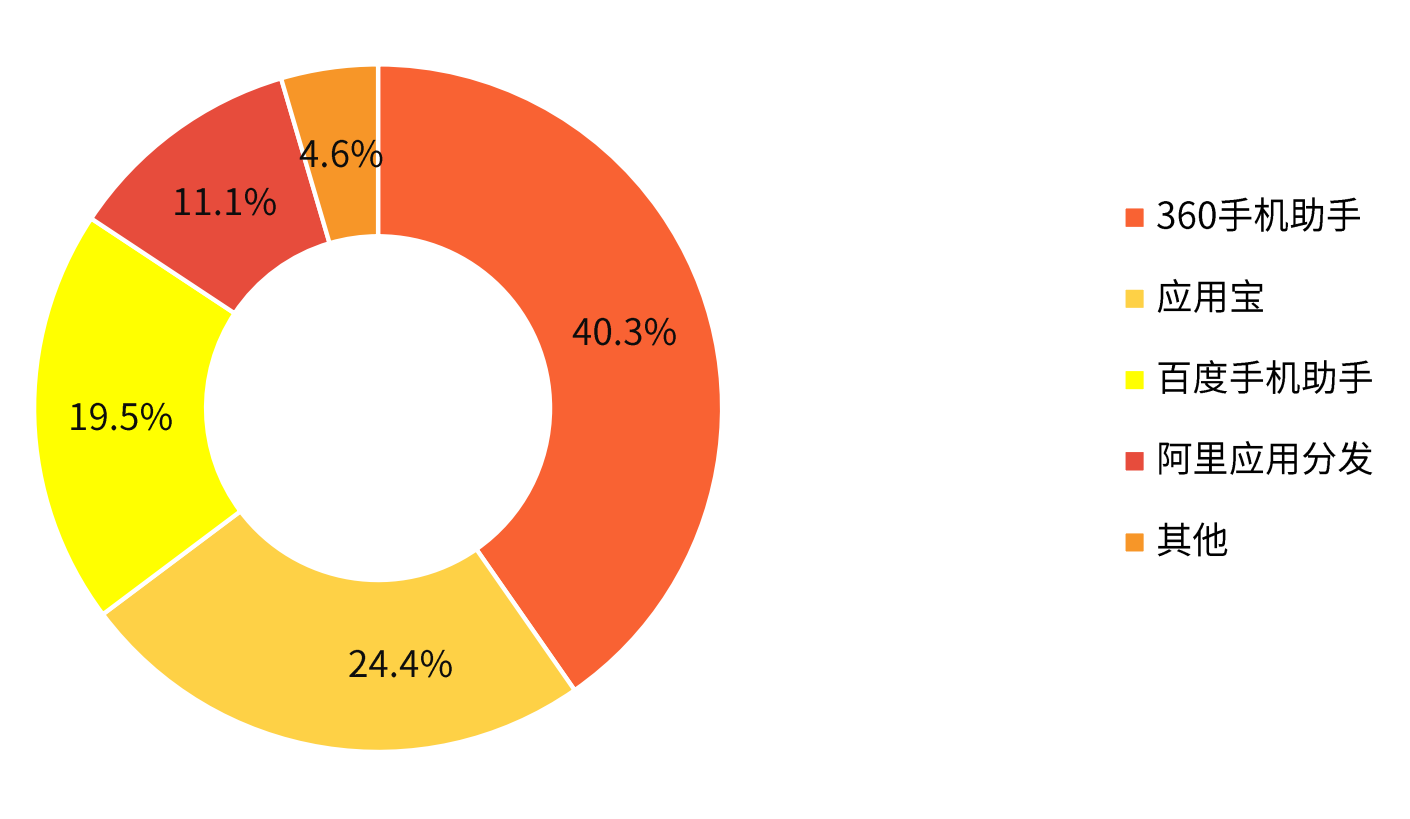
\includegraphics[width=0.5\textwidth]{./Figures/edwin-CHN-mkt-dist.png}
	\caption{2018中国第三方移动应用商店用户首选使用品牌分布}
	\label{fig:CHN-Mkt-Dist}
\end{figure}

与Google Play提供一个完整的Android生态环境相似,上述的各个厂商也致力于构建各自的Android应用生态链条:各大厂商本身就具有一定知名度,从其旗下的应用市场下载应用能让用户放心;开放开发者中心,让开发者注册账号后上传自己制作的App;为每一个App提供评分和评论功能,构建出开发者和用户的交流平台;在应用市场首页设置应用排行榜、推荐安装软件等榜单(如图~\ref{fig:mkt-yyb}),提高优秀App的曝光率;应用市场自带的应用版本管理开发者在市场后台更新应用之后,将更新推送到用户的手机上;各大应用市场也会整合支付平台(如支付宝和微信支付)来应对市场内的应用购买业务,华为应用市场甚至像Google Play一样,为市场上的应用提供了自家的支付渠道以支持应用内的付款项目购买功能。

\begin{figure}[htbp]
	\centering
	
\includegraphics[width=0.8\textwidth]{./Figures/edwin-yyb.jpg}
	\caption{腾讯应用宝应用市场首页(从桌面端浏览)}
	\label{fig:mkt-yyb}
	\vspace{-5mm}
\end{figure}

不同于在Android系统发布早期就存在的Google Play应用商店,国内的第三方应用商店是后期出现的产物,一出现就面临着激烈的市场竞争。
一方面,在国内各类第三方应用市场方兴未艾之时,国内的Android开发者社群尚未成熟,应用市场还未有大量开发者进驻;
另一方面,在成立初期,为了抢占市场份额,各个应用商店都想方设法将商店内App的种类和数量最大化,以迎合市场用户各种各样的需求。
作为结果,各类第三方应用市场都在各个渠道搜集App,而非通过开发者上传的方式获得货架上的应用程序。
由于在早期各种监管渠道尚未完善,各个市场在搜罗各类App的同时,难免会将大量的盗版应用也一并收录。

\section{Android App签名机制}

前文提到,开发者在使用Android SDK构建App时,其中十分重要的一步是对App进行数字签名。
实际上,Android的数字签名和安全证书机制基于RSA公共密钥系统,是Android安全机制中不可或缺的一个部分。
本章的余下内容将会对Android App的签名机制进行简单分析。

Android App的签名机制是用作校验APK文件是否被篡改、保证APK文件完整性的一个重要机制,所有的应用都必须要在经过签名才能安装进Android系统中。
在签名时,SDK会使用一种密钥库文件,如果开发者还没有这个文件的话,SDK会自动生成一个。
密钥库中包含了开发者的各种信息,包括一对公钥和私钥。
私钥用于数字签名,不可向外公布;公钥则是可以向外公布的一组密钥,用于数字前面的验证。
App中的签名也是系统用来识别开发者的重要依据,因为同一个密钥库文件会产生一致的签名,系统能根据签名中的公钥验证应用识别开发者。

签名的过程大致如下:
在前文流程的第二步结束后,编译器会输出DEX文件和编译好的资源文件,这时,SDK会对每个文件都扫描一次,然后对每个文件提取一次数字摘要,再把每个文件的文件名和其对应的数字摘要保存在一个名为\textit{MANIFEST.MF}的文件中。
之后,SDK会再扫描一次刚才生成的\textit{MANIFEST.MF}文件,再次提取一次数字摘要,把这个摘要连同刚才文件中的所有内容存入另一个新文件\textit{CERT.SF}里。
第三步,再计算一次\textit{CERT.SF}的数字摘要,然后用密钥库中的私钥对这个摘要进行加密。
加密后的结果就是数字签名。
最后,SDK将签名、公钥、计算数字摘要的哈希算法等信息写入\textit{CERT.RSA}文件中,再将这整个过程中生成的四个文件放进\textit{META-INF}文件夹,用APK打包器打包起来。
至此流程结束。

而Android系统验证签名的方式,则是先通过\textit{CERT.RSA}中的公钥验证签名是否无误,再根据文件中提供的哈希算法计算APK包中所有文件的数字摘要:先从\textit{CERT.SF}开始,然后是\textit{MANIFEST.MF},然后是APK中的其他所有文件...
一旦其中出现不相符的结果,就会导致验证失败。
在安装App的过程中,验证签名失败会使得系统终止App的安装。

换句话说,在一个APK被打包签名完毕之后,如果需要更改其中的内容,就只能在更改后将APK重新打包签名一次,即使是一个bit的修改也会破坏原有的签名。
这也是系统可以用数字签名识别开发者的原因:签名一致的App,最后一定都是由同一个开发者打包的。
所以,具有同样签名的App也可以在同一个Android设备上共享数据。
不过这超出了本文讨论的内容,故按下不表。

目前,签名的模式共有三代,其区别主要在于构建流程第三、第四步之间的一些操作上。
简单地说,越新的签名模式能越好地保障APK文件的完整性。
实际上,第一代签名模式V1具有较为致命的缺陷,所以Google官方也在呼吁开发者在编译时采用最新的签名模式。

要注意的是,签名机制只能保证APK文件在被篡改之后不能凭借原有的签名被安装进Android系统,但恶意开发者依然可以在篡改APK之后,用自己的密钥库对APK重新签名,构建出可安装的App。
这种App是盗版App的一种,被称为重打包App。

\section{本章小结}

本章主要介绍了Android系统、Android应用和Android应用市场的相关背景知识,同时也阐述了Android应用的构建流程和简要介绍了其中使用到的签名机制,为后文实证研究中使用到的采样来源和验证方法做铺垫。

\clearPaperPage

% \chapter{面向仿冒应用的收集框架\mytool}
\label{chp:fakerevealer}

\section{设计缘由}
鉴于目前学术界中未有相关工作能提供仿冒应用的相关数据集,本研究需要率先尝试从工业界中系统地收集所需的仿冒应用数据。
然而,传统的网络爬虫框架只能机械、不加区分地爬取数据,不能具有针对性地爬取与本研究中的目标应用相关的样本;应用市场中应用数量太多,完全收集并不可行。
为了解决这个问题,本研究提出了面向仿冒应用的收集框架\mytool,创新地采用启发式的方法搜索与爬取与目标应用相关的样本,为后文的两项研究服务。

\section{应用收集流程简介}
仿冒应用是一个跟正版应用相对的概念,所以本文需要先定义正版应用,再根据正版应用的信息搜寻仿冒应用。

1)\ \emph{正版应用收集} \quad
在定义正版应用方面,本研究参考了数据平台易观千帆的月度App排行榜~\cite{yiguanqianfan},然后从中选出了其中的前50款热门App作为本次研究的目标应用。
之后,本研究逐一地从这50款App的官方网站上下载了这些应用的最新版本,作为正版应用的参考版本。

2)\ \emph{仿冒应用收集} \quad
要获取足量的仿冒应用数据以组成数据集是一个十分具有挑战性的任务,难点如下:
\begin{itemize}
	\item 要从多个不同的应用市场中爬取App样本,但每个应用市场都有不同的网页编码,不存在一个爬虫脚本对所有应用市场数据都通用的场景;
	\item 各个应用市场架上的App数量浩如繁星,需要有效地找到和目标应用有关的所有样本,不重不漏;
	\item 对于大量数据,需要一个轻量级的解决方案快速判断获得的App样本究竟为正版应用又或者是仿冒应用。
\end{itemize}

为了应对第一个挑战,本研究与工业界合作,利用犇众信息公司的Janus平台对各大应用商店进行样本爬取,从而获得大量应用样本。
事实上,如\autoref{fig:Janus-data}显示,Janus平台自2017年起就开始对各大应用商店的App进行样本收集,至今已收集到上千万个App样本。
除样本搜集外,Janus也提供按规则搜索功能,用户可以创建自己的规则过滤平台中的应用数据,以获取自己需要的App样本。

\begin{figure}[htbp]
	\centering
	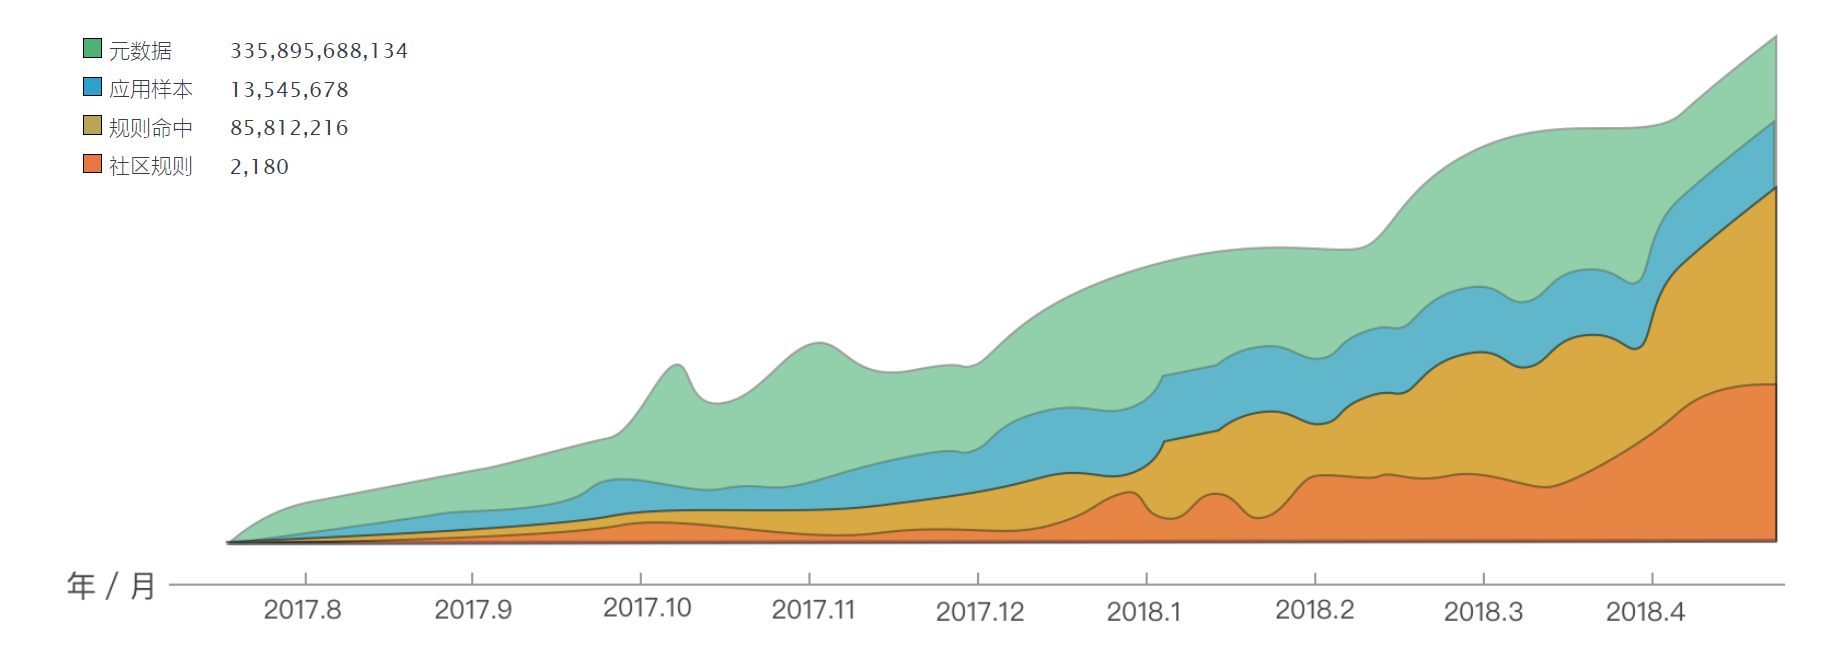
\includegraphics[width=\textwidth]{./Figures/edwin-Janus-data.png}
	\caption{Janus平台上的数据规模时序图}
	\label{fig:Janus-data}
	\vspace{-5mm}
\end{figure}

为了应对第二个和第三个挑战,本研究搭建了面向仿冒应用的收集框架\mytool。


\section{\mytool 的设计与实现}

本文使用Python 3开发了仿冒应用收集框架\mytool,该框架由\componentA 、\componentB 和\componentC 三个组件组成,\autoref{fig:FakeRevealer}展示了\mytool 的整体流程图。
输入初始正版应用的信息,\mytool 在经过迭代搜索、样本下载、应用过滤三个步骤之后,以CSV文件和JSON文件的形式输出仿冒应用各数据项和拓展后的正版应用信息。

\begin{figure}[htbp]
	\centering
	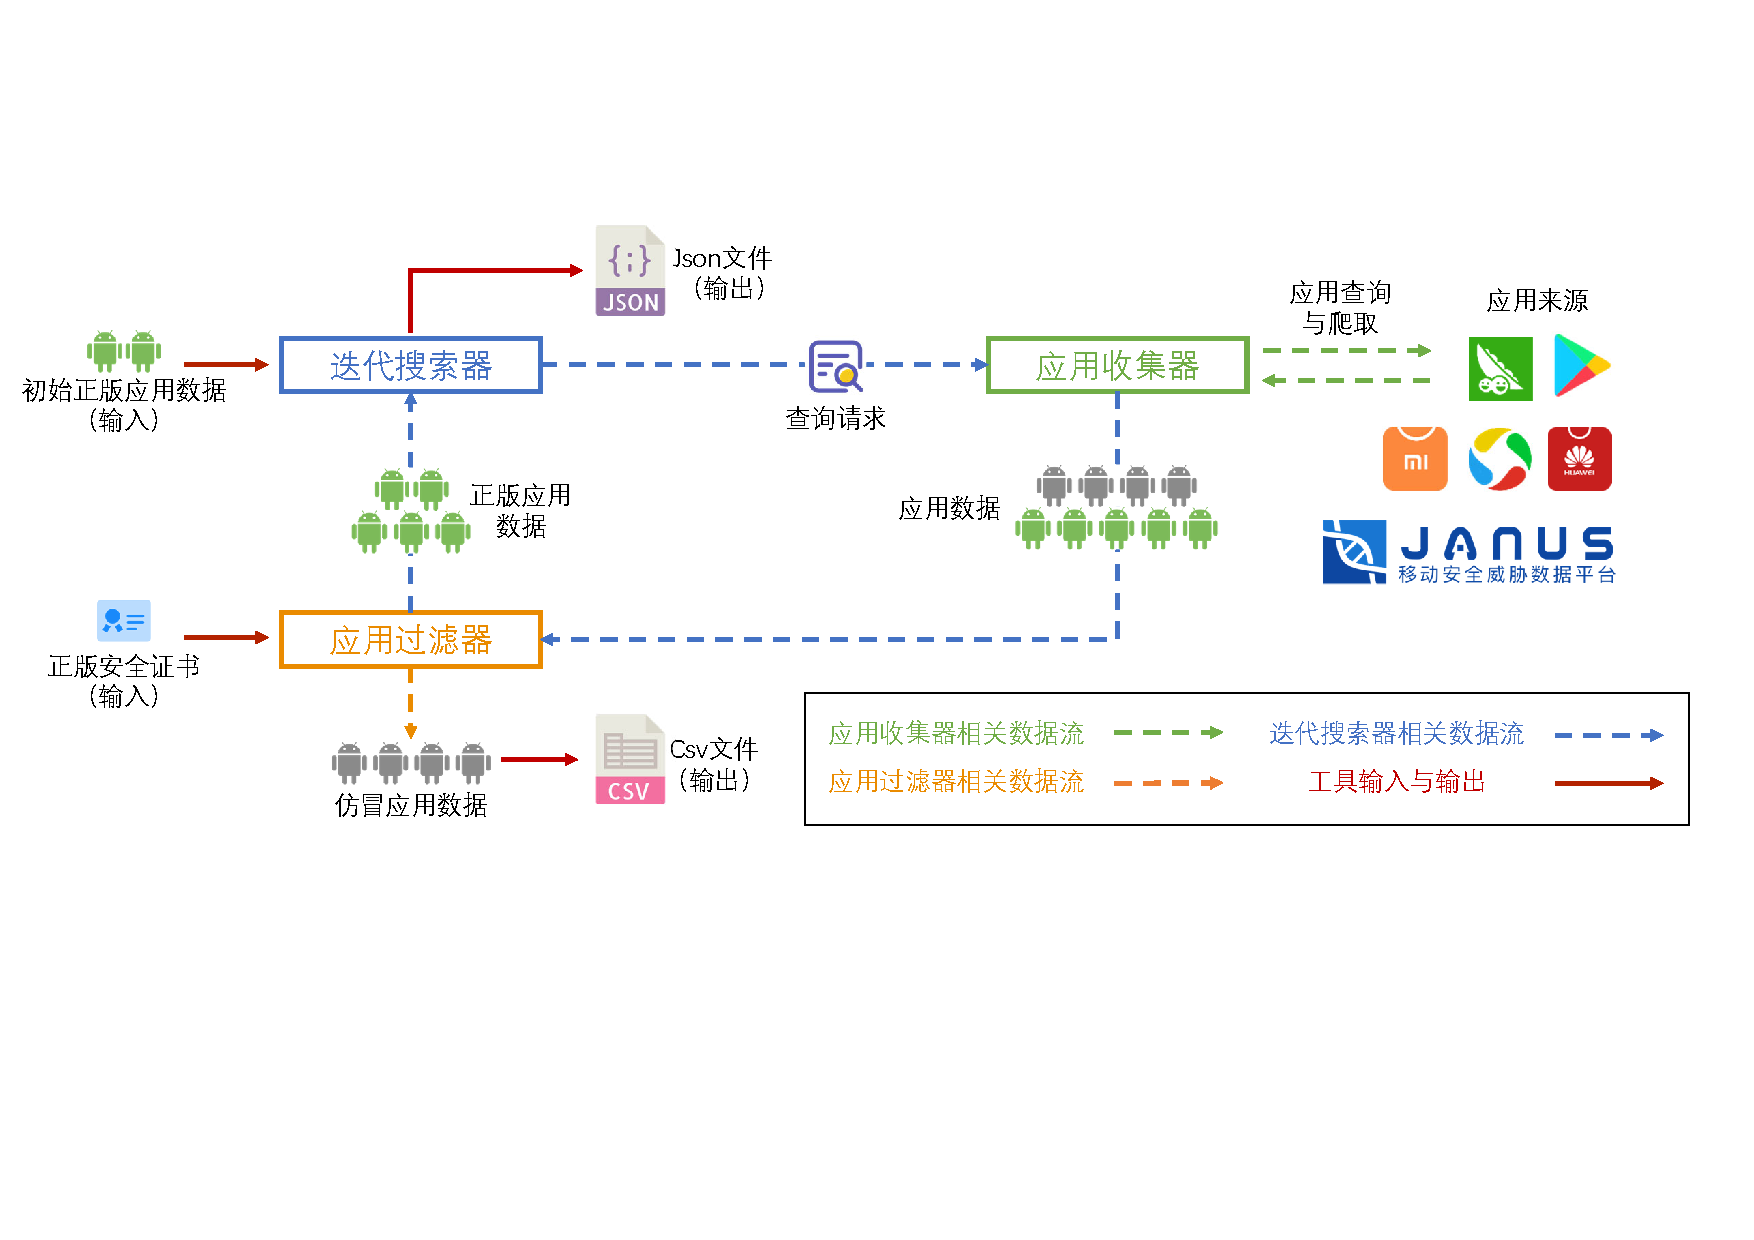
\includegraphics[width=\textwidth]{./Figures/edwin-fakerevealer}
	\caption{\mytool 整体结构}
	\label{fig:FakeRevealer}
	\vspace{-3mm}
\end{figure}

\subsection{\componentA }
\componentA 是与应用来源直接交互的部分,分为两个不同的子模块,分别是网络爬虫模块和APK包预处理模块。
在接收到应用收集请求之后,\componentA 会先根据收集请求,利用网络爬虫模块下载应用,然后再用APK包预处理模块对下载完毕的APK包提取信息,方便后续操作。

1)\ \emph{网络爬虫模块} \quad
本模块负责接收\componentA 的输入,根据输入中的需求从应用来源中查询并下载对应的App。
由于Janus平台上已经有提前收集好的源于各个应用市场的App样本,本研究直接从Janus上爬取应用。

不同应用商店提供应用查询、下载的API不同,不存在可以对应所有应用市场的爬虫脚本。
但只要研究者能分析出某应用商店查询、下载API的名称和用法,结合应用商店账户的Cookies,就能从该商店中下载应用。
考虑到这个方面,本研究设计了插件化的爬虫模块。
针对不同的应用商店,使用者可以在使用网络包分析工具(如Burpsuite~\cite{burpsuite})解析到API与Cookies信息之后,将对应API和Cookies写入配置插件,再对网络爬虫模块配置对应当前商店的插件,开始爬取应用。

在具体实现方面,本研究利用Python自带的urllib库实现对网络资源的访问;由于下载是可以并发进行的事务,为了能提高运行效率,代码实现利用了threading库对网络爬虫模块提供了多线程特性。

2)\ \emph{APK包预处理模块} \quad
这个模块负责从下载完毕的APK包中提取指定的数据项,存入键值对中,最后将所有应用的数据键值对以列表形式返回,作为\componentA 的输出。
APK文件中虽然包含着应用的所有信息,但本研究中的应用筛选并不需要用到整个APK文件,所以本模块会把筛选需要用到的数据先提取出来,后续处理时直接调用与该APK包有关的数据即可。
同时,由于不同APK包的大小不一,所需下载时长也各异,本框架在较大的应用还在下载的同时,对已经下载完毕的APK提取信息。
比起让\componentA 直接返回下载完毕的APK包、待后续需要数据时再进行数据提取的方法,这样的设计可以减小内存占用,也提高了框架的运行效率。

具体实现方面,APK包预处理模块使用Python的os库实现对命令行指令的调用,然后利用Android SDK中自带的命令行工具aapt对APK包进行解析,获取指定的数据项。


\subsection{\componentB }
这个组件的设计利用了一个基于广度优先搜索(Breadth-First Search,简称BFS)的算法,详情可见\autoref{alg:bfs}。
根据缓存中的正版应用信息,本组件向\componentA 提交查询、下载样本的请求。
在利用\componentC 过滤获得的应用信息后,再根据其中正版应用的信息扩增缓存中的数据,进行下一轮迭代搜索。

\begin{algorithm}[!ht]
	\tablewuhao
	\caption{迭代搜索算法}
	\label{alg:bfs}
    \KwIn{ $targetItems$,列表,用于拓展的数据项}
    \KwIn{ $legalApkInfo$,列表,包含正版应用及其信息键值对}
	\KwOut{ $cache$,列表,缓存拓展后的正版应用信息键值对}
	\SetKwProg{Fn}{Function}{:}{}

	\Fn {iterSearcher($legalApkInfo, targetItems$)} {

        $wtQueue$ = $\emptyset$;

        $cache$ = $\emptyset$;

        \For {$apkInfo \in legalApkInfo$} {

            \For {$item \in targetItems$} {

                $wtQueue$.add(${item: apkInfo[item]}$);

            }

        }

    	\While {$wtQueue \ne \emptyset$} {

    		$key, val$ = $wtQueue$.pop();

    		\If{${key: val} \in cache$} {continue;}

    		$cache$.add(${key: val}$);

    		$newSamples \gets$ appRetriever($key, val$);

    		\For {$sample \in newSamples$} {

                $isLegal \gets $ FakeFilter($sample$).getResult();

    			\If {$isLegal$} {

    				$sampleInfo \gets sample$.getInfo();

    				\For {$item \in targetItems$} {

    					$wtQueue$.add(${item: sampleInfo[item]}$);

    				}

    			}

    		}

    	}

    \KwRet{$cache$};

    }

\end{algorithm}

\autoref{alg:bfs}的输入有两项,分别是已有的正版应用信息列表$legalAppInfo$和要用来拓展搜索范围的数据项$targetItems$。

算法开始前,本框架先遍历每个正版应用的信息,将每个要拓展搜索的数据项对应的内容$apkInfo[item]$插入到待查询队列$wtQueue$中,完成初始化(第4 - 6行)。
然后是迭代搜索应用。
每次迭代中,本算法都从$wtQueue$中取出一组键值对,其中键$key$为本次迭代中用于搜索新应用的数据项,$val$为数据项对应的值(第8行)。
取出键值对之后,算法先检查该键值对是否已经被用于之前的搜索中。
如果该键值对之前已经出现过,就跳过本轮迭代,重新取一组键值对进行搜索;
否则,将本组键值对放入数据缓存$cache$,表示该组键值对已被使用过。
之后,组件将键值对传递给\componentA ,\componentA 会生成对应查询,从应用来源中获取数据项相关的应用(第12行)。
对于\componentA 返回的应用集$newSamples$中的每个样本$sample$,本文会用\componentC 检查$sample$是否为正版样本。
如果是正版样本,那么本算法将从该样本中获取对应的数据$sampleInfo$,然后将其中与待拓展对应项$item$对应的内容插入到待查询队列$wtQueue$中(第15 - 18行)。
当应用集$newSamples$中的所有样本都被筛选检查过之后,本轮迭代结束。
如果$wtQueue$中的所有键值对都已经被检索完毕(即$wtQueue$为空),本算法流程结束,本组件会将$cache$中被用于拓展搜索的各个数据项键值对整理成JSON文件输出,方便之后的再利用。

在本次实证研究场景中,$targetItems$包含两项内容,一个是应用的包名(\emph{PackageName}),另一个是应用自身的名字(\emph{AppName})。
之所以要这样操作,是因为开发者推出的App的应用名和包名并不是一成不变的。
一些热门应用会出于商业原因频繁地更改自己的应用名(比如爱奇艺视频,会根据其近期热播的电视剧/电影变更其应用名以吸引更多用户使用);
也有个别的热门应用可能会更换自己的包名,比如App有重大改版、又或者是开发者安全证书有变更,开发者不得不更换包名(具体原因可参考\secref{sec:signature}的Android App签名机制部分)。

\subsection{\componentC }
顾名思义,\componentC 的功能是从输入的应用程序集之中将仿冒应用筛选出来,其核心是安全证书的识别。
根据\secref{sec:signature}中对Android应用签名机制的描述,一个App中包含的安全证书文件指示了对APK文件进行修改的开发者。
如果一个APK文件中包含的安全证书信息与指定应用的开发者信息相符,那么本组件认为这个APK包来源于正版的开发者;否则本组件认为这是一个仿冒应用。

在开始过滤之前,开发者需要先向过滤器导入正版证书信息。
针对上一节提及开发者安全证书可能有变更的情况,本研究仔细排查了所有目标应用,以确保初始化\mytool 时没有正版证书被遗漏。
之后,对于每个输入的应用,组件会将其安全证书信息和正版证书信息作比对。
对于证书信息相符的应用,本组件会将其放入\componentB 的待检索队列中用作下一轮的迭代搜索;
而证书信息不相符的应用则会被筛选出并保存。

在迭代搜索的流程结束之后,本组件会将保存的所有仿冒应用数据项导出成CSV文件保存,方便之后的数据挖掘。


\section{仿冒应用数据概览}
以下是框架收集到的数据的概览:

从易观千帆提供的数据榜单中,本研究选择了50个最热门的App作为目标应用,这些App分属11个不同的应用类别。
由于App的应用名可能会在App更新迭代的时候随之变更,本研究用基于BFS的策略,从50种App中一共记录了198个不同的应用名,来挖掘仿冒样本。

在这50款App中,以下三款App的样本并不能在市面上找到:\emph{OPPO 应用商店},\emph{华为应用商店}和\emph{小米应用商店}。
因为这三款App都是由手机设备厂商开发和预装在对应品牌的手机中的,仅供这些品牌的用户使用,并不在其他应用市场上提供下载。
当然,这也是这三款App热度高的原因——这几款App都被预装到了对应手机品牌厂商的每一部Android设备中,而OPPO、华为和小米又是国内最大的几家手机厂商,这几款App自然也会有庞大的用户基数。
因此,本研究最后的目标应用只有47款。

对这47款目标应用,本研究总共收集到了138,106个应用样本。
其中,69,614个应用样本持有官方开发者证书,52,638个应用样本并不具有官方证书。
还有一部分应用样本,是某些应用的分别发布在不同应用市场同一版本,在经过去重筛选后被排除(共计15,854个)。

对于每个样本,框架收集8个数据项作为元数据:\emph{样本SHA1码},\emph{安全证书SHA1码},\emph{包名},\emph{样本大小},\emph{版本号},\emph{搜集时间}和\emph{APK包来源}。
其中,\emph{样本SHA1码}是使用SHA1哈希算法对整个APK文件进行数据摘要之后获取到的编码串,每个样本都有独一无二的SHA1码;安全证书SHA1码则是对样本的安全证书采用SHA1算法提取数据摘要之后获取的编码串,用于识别不同的证书。
而\emph{搜集时间}则是样本从应用市场被爬取到数据库的时间点,\emph{APK包来源}指示该APK包来源的应用市场。


\section{本章小结}
本章介绍了数据收集的流程和方法,然后讲述了面向仿冒应用的收集框架\mytool 的工作流程,以及其中三个组件——\componentA 、\componentB 和\componentC 的设计实现,最后对采集到的数据进行了简要描绘。

尽管\mytool 在设计之时选择了利用包名和应用名迭代搜索、通过安全证书筛选的机制过滤仿冒应用,但框架本身的流程并不囿于此机制中,读者可以参考本框架流程,设计其他过滤仿冒应用,或者是其他任何具有某种特征的应用的工具。

在明确数据收集流程之后,本研究针对仿冒样本中采集到的元数据进行了挖掘分析,以求获得对于仿冒应用生态和特征、以及对于仿冒应用开发者的行为的更全面的认知。
下一章内容将提供有关挖掘分析的详情、本文从数据中分析出的结论以及相关案例。

% \clearPaperPage

% \section{Large-scale Empirical Study and Discoveries}
\chapter{大规模实证研究与发现}
\label{chp:discoveries}

% With the large-scale dataset ready, we can further conduct a comprehensive empirical study to acquire the nature of fake apps as well as understanding their ecosystem.
在数据库准备好之后,我们就可以对这些仿冒应用进行大规模分析,挖掘仿冒应用的信息并了解其生态系统了。
% To effectively measure different facades of fake apps, We define three perspectives, namely \emph{Fake Sample Characteristics}, \emph{Quantitative Study on Fake Samples}, and \emph{Developing Trend}.
为了能更全面有效地测量这些仿冒应用的各方面,我们定义了三个不同视角,即:\emph{仿冒应用的基本特征}、\emph{针对仿冒样本的量化分析}和\emph{仿冒应用的发展轨迹}。
% Next, we'll describe each perspective in detail.
接下来,我们会详细描述各个不同视角的观察方法以及观测结果。

% \subsection{Fake Sample Characteristics}
\section{仿冒应用的基本特征}
\label{sec:fakeCharacteristics}
% To reveal the strategy the fake app authors are employing, or how they bypass app markets' security scheme, fake sample characteristics have to be understood.
为了了解仿冒应用作者使用的仿冒策略,或者说,他们是如何绕过应用市场的监管机制的,我们有必要对仿冒应用的基本特征有所了解。
% As such, we conduct our measurement in terms of certificates and basic information like app names, package names and package sizes.
为此,我们分别针对应用的安全证书和应用名称、包名和应用大小等基本信息进行了观测.

% Certificate serves as the identifier for developers.
应用的安全证书就是对开发者的识别码,
% The nature of the certificate, namely, whether each fake app has a unique certificate, is likely to be essential to fake apps' evasive technique.
而仿冒应用在安全证书上的性质(也就是说,是否每个仿冒应用都有一个独一无二的安全证书),十分可能是仿冒应用规避监管技术的关键。
% On the other hand, we believe repackaged apps, as a kind of \texttt{imposters}, are widespread in our dataset.
另一方面,我们也猜想打包应用(一种\texttt{高仿应用})在我们的数据集中普遍存在。
% Measurement on basic information of fake apps, such as package names and package sizes, helps us determine how repackaged apps are distributed, since repackaging an app does not change any of its basic information (i.e. the app name, package name, version code, etc.) unless it's done intentionally.
对仿冒应用基本信息的测量,比如说对应用包名和大小的测量,则可以帮助我们了解重打包应用在数据集中的分布如何。
因为普通的重打包技术并不会对APK的基本信息(比如应用名、应用版本号等)作出修改,除非仿冒作者有意为之。

\subsection{安全证书与仿冒应用的对应关系}
那么,安全证书和仿冒应用的对应关系如何?
对此,我们提出了假设:

% \noindent{\bf Hypo 1.1:} Most of these fake samples have their corresponding unique certificates.
{\bf 假设 1.1}: 绝大部分的仿冒样本有其对应的、独一无二的安全证书。
% In other words, most fake certificates and fake samples have a one-to-one relation.
换句话说,绝大部分仿冒应用和他们的安全证书呈一对一的映射关系。

与之对应,我们提出了以下的研究问题:

% \noindent{\bf RQ 1.1}: What's the relationship between the number of fake samples and their certificates? That is, how many fake samples does one certificate usually link to?
{\bf RQ 1.1}:仿冒样本数量和他们的安全证书数量存在着什么样的关系?也就是说,一个安全证书通常会跟多少个仿冒应用样本相关联?

为了解答这个问题,我们从所有搜集到的样本中提取出安全证书,然后对这些证书和样本做了配对。
根据配对得出的数据,我们得出了以下结果:

% \noindent{\bf Answer to RQ 1.1.}
{\bf RQ 1.1. 结果}
% 76\% of these fake certificates are linked to merely one or two fake samples, and the number of fake examples a certificate links to is various from 1 to 1,374.
在仿冒应用持有的所有安全证书中,76\%都仅仅关联到了一到两个仿冒样本,与单个安全证书相关联的仿冒应用数分布在从1到1,374的区间内。
% We count the number of certificates which link to different sample number in table~\autoref{table:certificate_number_statistic}.
我们在\autoref{table:certificate_number_statistic}中统计了安全证书和他们对应的仿冒样本数量。
其中第一栏为仿冒样本的数量区间,第二栏为关联的仿冒样本数量该落于区间的安全证书数。
大部分安全证书都只关联了1到5个应用样本,但也有少量安全证书与大量仿冒样本有关联关系。

\begin{table}[htbp]
  \renewcommand{\arraystretch}{1}
  \footnotesize
  \centering
  \caption{安全证书/仿冒应用数量对应表}
  \vspace{1mm}
  \begin{tabular}{l c c c c c c c}
  \toprule
  {\bf 仿冒样本数量} & {\bf 1-5} & {\bf 6-10} & {\bf 11-50} & {\bf 51-100} & {\bf More than 100} \\
  \midrule
  {\bf 安全证书数量} & 8252 & 525 & 531 & 71 & 80 \\
  \bottomrule
  \end{tabular}
  \label{table:certificate_number_statistic}
\end{table}

% This discovery partly matches our assumption that most of these fake samples have their corresponding unique certificates.
这个发现与我们的猜想(即大多数仿冒样本都有他们对应的独一无二的安全证书)部分相符。
虽然并不是大多数仿冒样本都有其单独对应的安全证书,但多数安全证书的确只对应少量样本。
% We consider this as a strategy to bypass app markets' security scheme, as even if one fake sample is exposed, other fake samples developed by the same developer will not be implicated directly.
结合\secref{sec:signature}Android App签名机制最后的说明,我们认为这是规避应用市场监管机制的一个策略。
如果以同一开发者的身份,用一个安全证书上传多个仿冒App,万一其中App被投诉下架,其他的App很可能会受到牵连。
然而,一个仿冒开发者其实也可以持有多个安全证书。
如果使用多个安全证书分别上传仿冒App,应用市场就不容易找到这些App的关联,即使其中一部分被举报下架,余下的也得以被保全。
% Nevertheless, when reviewing certificates linked with multiple fake samples, we find some very surprising findings that we will expound in Section~\autoref{sec:casestudy}.
另外,在整理对应多个仿冒样本的安全证书时,我们得到了一些意料之外的发现。相关内容会在\fullref{chp:casestudy}中加以拓展。

\subsection{仿冒样本与原版应用的相似度}

除了安全证书以外,应用的外观也是十分重要的基本特征。
鉴于运算量等原因,我们暂时无法将应用图标和应用内布局等因素用于仿冒样本和原版应用的对比,但我们依然提取出了样本的包名/应用名/APK包大小等最基本的项目数据以比较仿冒样本和原版应用的相似度。
在这个方面,我们的假设如下:

% \noindent{\bf Hypo 1.2:} A large portion of fake samples have the same app names/package names/apk sizes as those in official samples.
{\bf 假设 1.2}: 一大部分的仿冒样本和他们的仿冒对象(也就是原版的官方App)有同样的应用名/包名/APK包大小。

与上一假设类似,我们也对应地提出了一个研究问题:

% \noindent{\bf RQ 1.2}: How do fake apps imitate official apps? That is, how similar are the names/package names/apk sizes of fake samples compared to those of official samples?
{\bf RQ 1.2}:在我们的数据集中,仿冒应用是怎么``山寨''正版App的?也就是说,仿冒应用的应用名/包名/APK大小和他们对应的正版App有多相似?

以编辑距离作为度量,我们对目标应用和仿冒样本的应用名/包名相似度作了比对,同时对比了两种样本的大小区别,得出了以下结果:

% \noindent{\bf Answer to RQ 1.2.}
{\bf RQ 1.2. 结果}
% According to our statistical result, only 243 out of 52,638 samples (less than 0.5\%) use official package names, all the rest fake samples (more than 99.5\%) use their own package names.
以包名为例,根据我们的统计结果,在所有的52,638个仿冒样本中,只有243个(少于0.5\%)使用了正版应用的包名,余下大于99.5\%占比的所有仿冒样本都使用了他们自定义的包名。
% In the rest 52,395 samples, 14,089 different package names were found.
在余下的这52,395个样本中,我们找到了14,089个不同的包名。
% But does this mean fake samples are all using package names that are totally different from the official ones? Could they be using package names that are similar to their official correspondences?
这其实在我们的意料之中。
因为每个应用在Android系统中都需要有独一无二的包名,如果系统在安装App时发现系统中已经有具有相同包名的App,就会检查两个不同版本应用的安全证书,证书不一致会导致安装失败。
因此大部分仿冒应用不会直接使用正版App的包名。
但这是否意味着仿冒应用就会使用与正版App完全不同的包名呢?
它们会不会使用和正版App相似的包名?

同理,我们对应用名和APK大小两个方面也有类似的疑问。
下面将会就我们获得的数据,探索上述问题。

% To figure out the similarity, we utilize \textit{edit distance}~\cite{levenshtein1966binary}, a distance definition widely applied in natural language processing (NLP):
为了解决相似度问题,我们采用了\textit{编辑距离}~\cite{levenshtein1966binary}这一在自然语言处理(Natural Language Processing,简称NLP)领域被广泛应用的距离定义作为衡量标准。

\begin{Def}
	编辑距离

	% {Given two strings $a$ and $b$, the edit distance $d(a, b)$ is the minimum-weight series of edit operations that transform $a$ into $b$.
	% In our case, edit operations refer to either to append, to delete or to change a character.}
	给定两个字符串$a$与$b$,其间的编辑距离$d(a, b)$为将$a$和$b$相互转换的最小编辑操作数。
	其中,每次添加、删除或将一个字符转换成另一个字符都算作一次编辑操作。
\end{Def}

% For instance, the edit distance between string ``fake" and ``official" is 7, while between ``jingdong" and ``jindeng", this value becomes 2.
举个例子,``jingdong''和``jindeng''之间的编辑距离是2,由前者转换为后者的其中一种编辑次数最小方法是将第一个``g''删除,然后再将``e''转成``o''。
同理,字符串``fake''和``official''之间的距离是7,其中一种方案是在``f''前添加``o'',在``f''和``a''之间添加``fici''(这里包含了4步操作),将``k''替换作``l'',最后删去``e''。
% For every fake package name from a fake sample, we compute its edit distance to the official package name of its original.
对于从仿冒样本中获取到的每个包名,我们都计算了与其对应的官方发布App的正版包名的编辑距离。

\begin{figure*}[htbp]
	\centering
    \subfloat[应用名\label{fig:appname}]{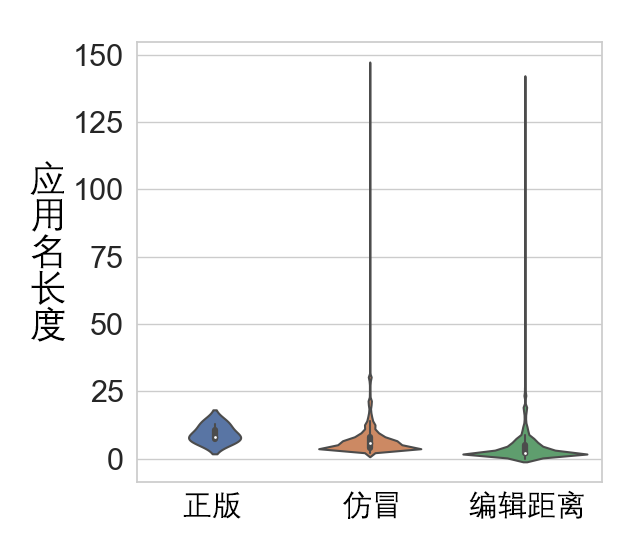
\includegraphics[width=0.333\textwidth]{./Figures/edwin-RQ1-2(a).png}}\hfill
    \subfloat[包名\label{fig:pkgname}]{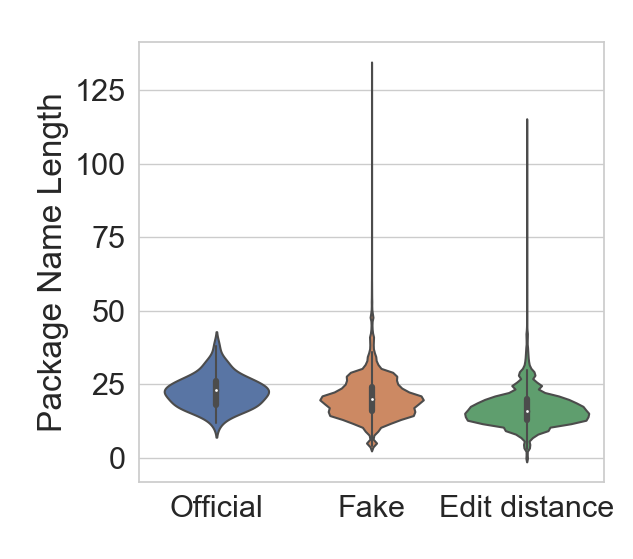
\includegraphics[width=0.333\textwidth]{./Figures/edwin-RQ1-2(b).png}}\hfill
    \subfloat[样本大小\label{fig:size}]{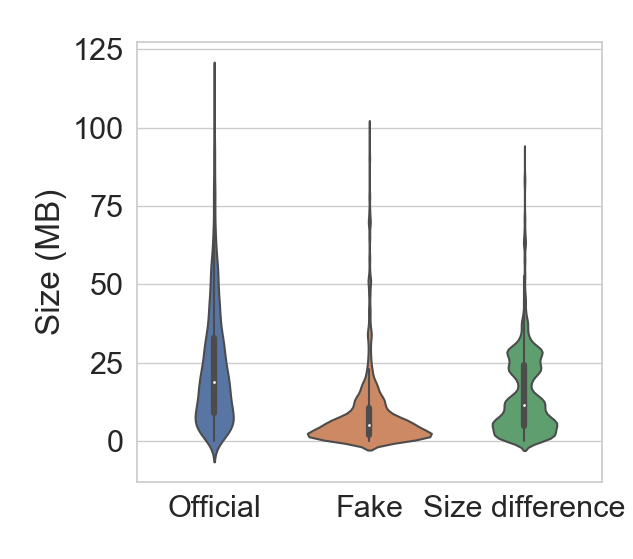
\includegraphics[width=0.333\textwidth]{./Figures/edwin-RQ1-2(c).png}}\hfill
	\caption{对App各项属性的统计结果}
	\label{fig:Statistic_fake_and_official}
	\vspace{-5mm}
\end{figure*}

% Fig.~\autoref{fig:Statistic_fake_and_official} is consist of three violin plots,\footnote{\url{https://en.wikipedia.org/wiki/Violin_plot/}} representing our statistics on app names, package names and package sizes, respectively.
\autoref{fig:Statistic_fake_and_official}由三个小提琴图\footnote{\url{https://en.wikipedia.org/wiki/Violin_plot}}组成,分别表示了我们在应用名、包名和APK包大小上的统计信息。
% In each ``violin'', the white dot represents the median, the thick bar in the middle represents the interquartile range while the thin bar represents 95\% confidence interval.
在每个``小提琴''中,中间的黑色粗条表示四分位数范围,粗条中间的小白点表示数据的中位数,而黑色细条表示95\%置信空间。

% Fig.~\autoref{fig:appname} shows the statistic information on app names of official samples, fake samples, and the edit distance between them.
\autoref{fig:appname}表示了分别在官方样本、仿冒样本的应用名和两者间编辑距离的统计数据。
% Both the white dot in ``Official'' violin and the one in ``Fake'' violin are at a similar level near the value ``6'', which means the average length of app names of both official samples and fake samples are close to each other.
其中``官方''图例和``仿冒''图例中的小白点都在接近数值``6''的位置,说明官方样本和仿冒样本的应用名的平均长度十分相近。
% The overall distribution of these two data groups have similar bodies, signals that they are also similar as well.
这两个数据组之间的数据分布的主体略微相近,也表面了他们的相似程度。
% What's more, the median value of edit distance is low (``2'' on $y$-axes), meaning that half of the fake apps get their names by modifying less than 3 characters from the corresponding official apps' names.
更重要的是,图中``编辑距离''图例的中位数值十分低(在$y$轴上为``2''的位置)。
这意味着过半数仿冒应用通过从官方App的应用名中修改少于3个字符来获得其应用名。
% This is a proof indicating that most fake apps are using a similar name to an official name.
这表示大部分仿冒应用正在使用与官方App非常相似的应用名。
% At the same time, we notice that some fake apps have pretty long names (there is one with a name of 146-character-long length).
与此同时,我们也留意到了一些仿冒应用有着异乎寻常的长名称(其中最长的仿冒样本的应用名中甚至有146个字符)。
% Many of those outliers are samples uploaded by fake authors, maybe for testing purpose to explore the vetting mechanism.
% The other purpose is to associate users' search keywords as far as possible.
我们认为这些异常样本有可能是出于测试市场审查机制的目的而被上传到市场上的。
另一种可能是,一些长应用名拼合了多个热门App的名称(比如``潮流女装-美丽说蘑菇街淘宝天猫京东美团精选''),这可能是为了应用更容易地被用户搜索到而采取的策略。

% Fig.~\autoref{fig:pkgname} shows the result on package names.
\autoref{fig:pkgname}显示了针对包名的结果。
% Like the plots in Fig.~\autoref{fig:appname}, the difference between the average length of package names of official apps and the average length of package names of fake apps is still tiny (they are of value ``23'' and ``20'', respectively).
和\autoref{fig:appname}类似,官方App的平均包名长度和仿冒样本的平均包名长度依然很类似(双方的值分别为``23''和``20'')。
% Nonetheless, the median of edit distance between them is explicitly higher (``16'' on $y$-axes), which means it takes averagely 16 times modification to turn a fake package name to an official package name and vice versa.
然而,他们之间编辑距离的中位数则比应用名编辑距离的中位数明显更高(在$y$轴上``16''的位置),这意味着将一个仿冒应用的包名转换为一个官方App的包名平均需要16次修改,反之亦然。
% Thus, we infer that fake apps tend to use self-defined package names.
也就是说,官方App的包名和仿冒应用的包名会相当不一样。我们可以据此推出仿冒应用更倾向于使用自定义的包名。

% Fig.~\autoref{fig:size} reports package size information.
\autoref{fig:size}显示了APK包大小的信息。
% To better represent the trend, we eliminated some outliers: samples that are larger than 150MB (851 in 69,614 official samples (about 1\%) and 447 in 52,638 fake samples (less than 1\%), most of which are from 游戏 category).
为了能更好地显示结果,我们作图前从数据集中剔除了一些极端样本:他们是大于150MB的APK包,在所有69,614个官方App的样本中占851个(约为1\%),在52,638个仿冒样本中占447个(少于1\%)。
这些极端样本大部分来源于``游戏''类别下。
% The figure shows that the median number of fake samples' size is around 5MB, while half of the official apps have a size greater than 18MB, meaning that fake apps are more likely to be
图表显示,仿冒样本大小的中位数约为5MB,而约半数的正版App有着大于18MB的大小。
因此,仿冒应用更有可能:

% (1) developed by their owners but not originated from repackaging official apps,
1)由仿冒开发者自行开发,而不是使用重打包技术制作,因为重打包之后的应用通常不会在大小上与原版有太大差距;

% (2) malicious apps, for malicious apps are usually in small sizes.
2)是恶意应用,因为恶意应用除了恶意代码之外,通常没有太多其他内容。

% In short, Fig.~\autoref{fig:Statistic_fake_and_official} tells that fake apps
简而言之,\autoref{fig:Statistic_fake_and_official}说明了仿冒应用:

% (1) prefer to use a similar (or even same) name to an official app's name, but they have their own package names and
1)更倾向于用一个与正版App相似(甚至是相同)的应用名,但会使用自定义的包名;

% (2) are usually of a small size.
2)通常大小更小。

\begin{figure*}[htbp]
	\centering
    \subfloat[360应用市场\label{fig:360_detail}]{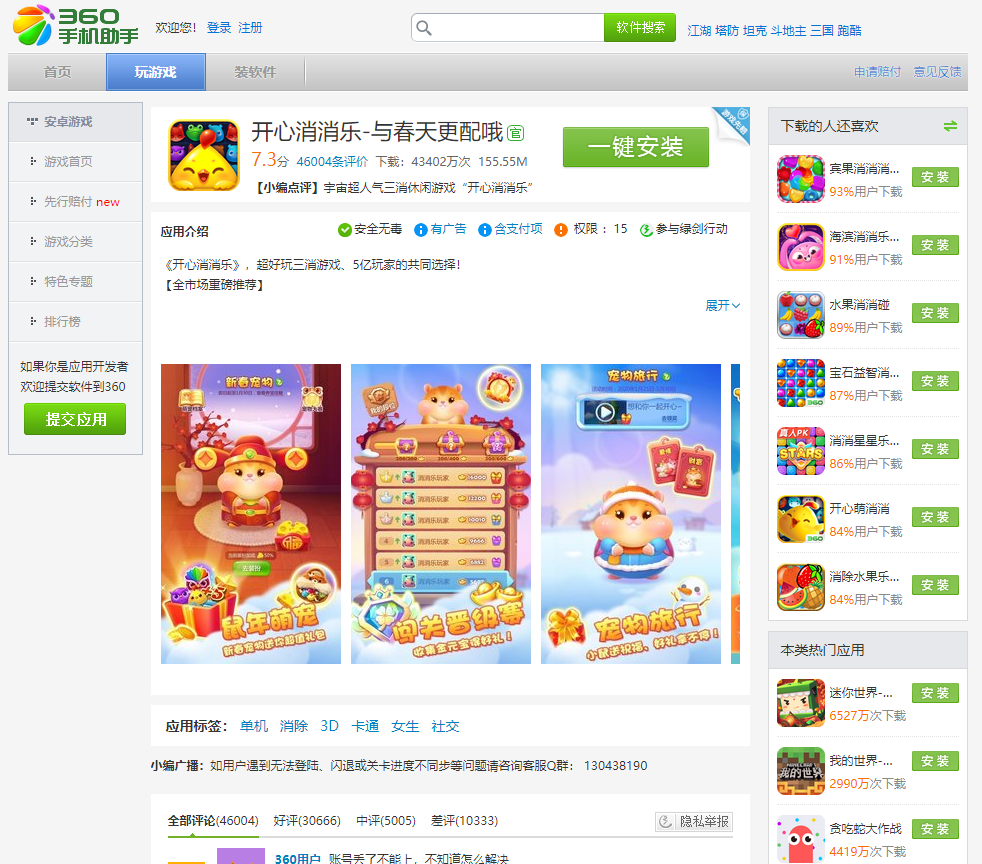
\includegraphics[width=0.49\textwidth]{./Figures/edwin-app-detail-360.png}}\hfill
    \subfloat[应用宝\label{fig:yyb_detail}]{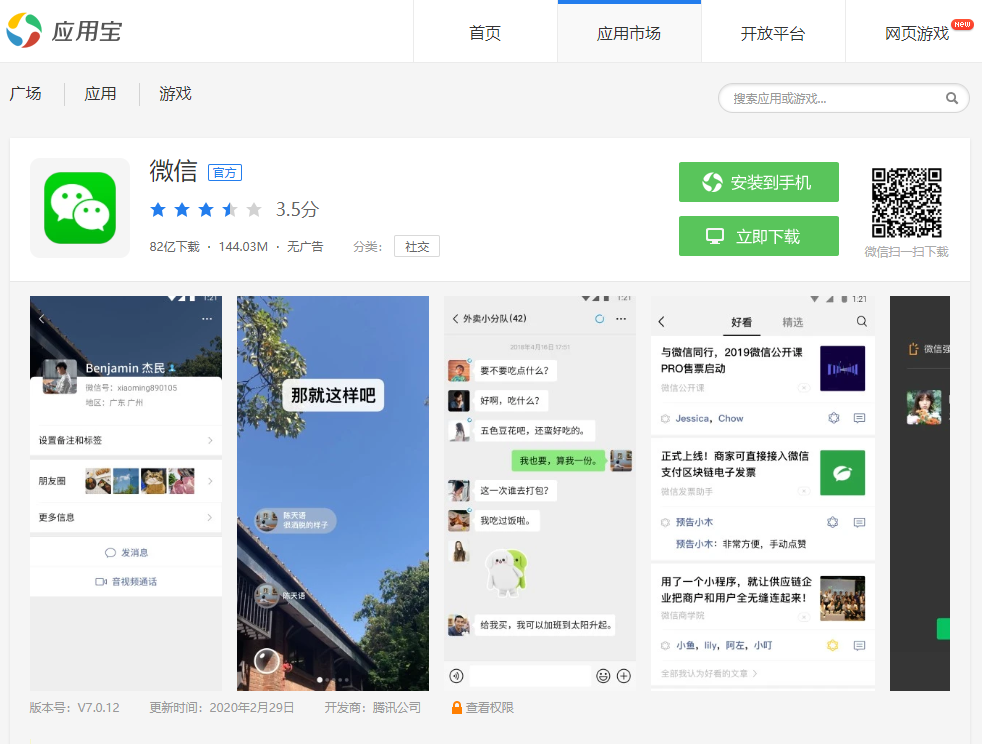
\includegraphics[width=0.49\textwidth]{./Figures/edwin-app-detail-yyb.png}}\hfill

	\subfloat[百度手机助手\label{fig:baidu_detail}]{
\includegraphics[width=0.49\textwidth]{./Figures/edwin-app-detail-baidu.png}}\hfill
    \subfloat[小米应用市场(部分信息被折叠)\label{fig:xiaomi_detail}]{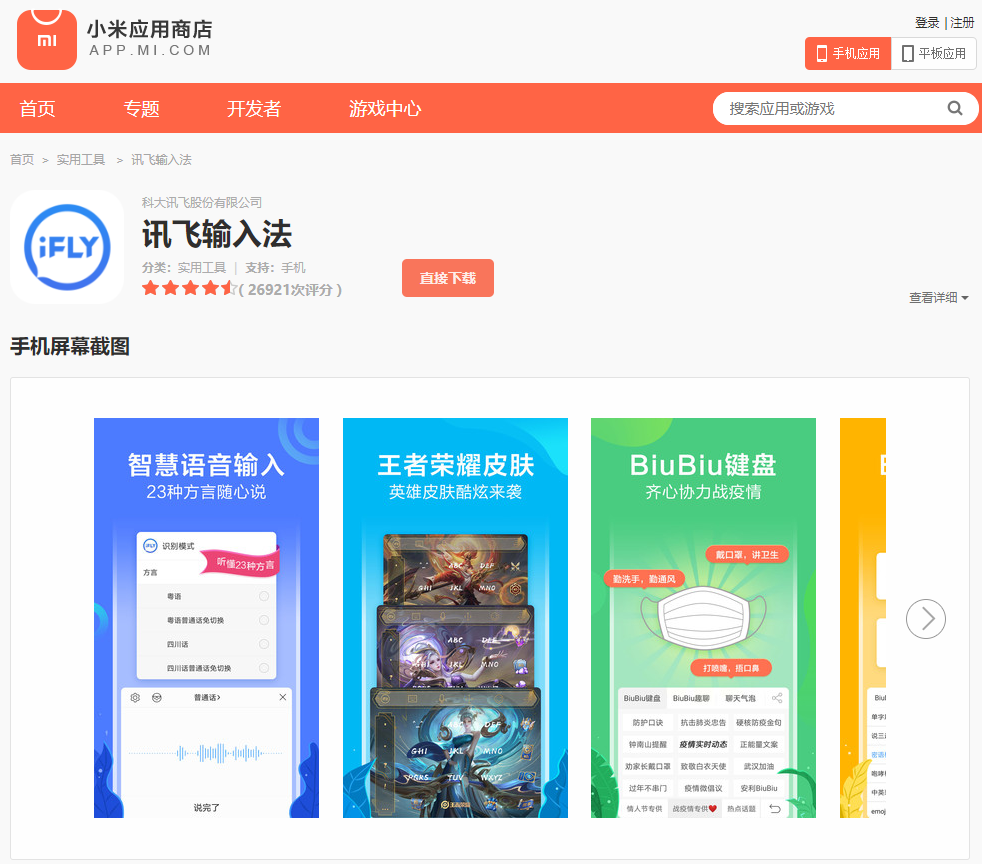
\includegraphics[width=0.49\textwidth]{./Figures/edwin-app-detail-xiaomi.png}}\hfill
	\caption{各大应用市场应用详情页(从桌面端浏览)}
	\label{fig:app_detail_page}
	\vspace{-5mm}
\end{figure*}

% To a large extent, we owe the first point to the incompleteness of the information the app store displays on apps.
在很大程度上,我们认为产生第一点结论的原因是应用市场上提供的App信息的缺失和用户对Android App了解的缺乏。
% In most app stores, when users browse an app's detail page, they can only see the app's name, description, user comments and ratings which are positive for leading users to download that app.
如\autoref{fig:app_detail_page}所示,在应用市场上,当用户浏览App的详情页时,能看到应用名、下载量、应用描述、其他用户对应用的评论和评分等信息。
% However, technical information rarely appears.
但是,大部分应用详情页上并不会出现技术详情,比如应用包名。而普通用户也不会了解Android App中包名和应用名的区别和关联。
% In some app markets, users don't even know how large an apk file is.
个别应用市场(如\autoref{fig:xiaomi_detail}所示的小米应用市场)上,应用的某些信息甚至被折叠了起来,用户要点开折叠页才能发现一个App会有多大。
因此,不会被普通用户关注的包名自然可能会出现各种五花八门的情况,而一定会显示的应用名则是越接近正版App越容易诱导用户下载。

\vspace{5mm}
\noindent\fbox{
	\parbox{0.95\linewidth}{
		% \textbf{Remark 1}: Most certificates link with only a number of fake apps, which is highly possible to be a fake developers' evasive strategy.
		\textbf{本节小结}: 绝大部分安全证书只与少数仿冒样本有所关联。这很可能是仿冒开发者规避市场监管机制采用的策略。
		% Moreover, we observe that fake apps do tend to use official app names or names alike.
		同时,我们也观测到仿冒应用倾向于于官方App相同或者是十分相似的应用名。
		% Nonetheless, fake apps and official apps are not resemble in terms of package names or apk sizes, disclosing that repackaged apps are not mainstream in fake apps.
		但是,仿冒样本和官方App在包名和APK包大小方面都不相似,这表明重打包应用在仿冒应用中并不普遍存在。

	}
}

% \subsection{Quantitative Study on Fake Samples}
\section{针对仿冒样本的量化分析}
\label{sec:quantitativeStudy}
% It is valid to assume that fake app developers are driven by profits, hence there is a likelihood that the number of fake app is correlated to their source market, popularity and categories.
天下熙熙,皆为利来;天下攘攘,皆为利往。我们不妨假设获利是驱动仿冒应用开发者的最终目标,进而假设仿冒应用的数目与其来源市场、受欢迎程度还有应用分类密切相关。
因为一个应用越受欢迎,就越可能获利,对仿冒应用也是如此。
% In addition, the update frequency can be taken in as a factor, too.
此外,App的更新频率也可以被视作一个潜在因素,频繁更新的App或许会阻碍仿冒应用开发者对其进行仿冒。

\subsection{仿冒应用的来源}

我们搜集的应用样本来源于多个不同的应用市场,每个市场架上的应用数量不一,其审核、监管力度也并不一致。
因此我们不禁好奇,应用商店架上的应用样本数量是否会跟仿冒应用的数量有关系?
为此我们有了以下假设:

% \noindent{\bf Hypo 2.1:} {The rate of fake samples is related to the number of apps a market contains.}
{\bf 假设 2.1}:仿冒样本的比率与应用市场架上的App数量有关联。

% Correspondingly, we define our research questions as follows:
与之相对,我们定义了研究问题:

% \noindent{\bf RQ 2.1}: Where are these fake samples mainly from?
{\bf RQ 2.1}:这些仿冒应用市场都集中来源于哪里?哪个应用市场有最多的仿冒应用?

根据各个样本的来源,我们从数据统计角度分析了结果。

% \noindent{\bf Answer to RQ 2.1.} Fig.~\autoref{fig:Sample_source} shows the samples' origin.
{\bf RQ 2.1. 结果} \autoref{fig:Sample_source} 展示了我们收集到的所有样本的来源。
% From the left subplot, \texttt{Baidu App Store} not only provides the largest sample number among all 31 different app sources, but is also the source where most fake samples are from.
在左边的图中,我们可以看到,在我们收集数据的所有31个应用商店中,源于\texttt{百度手机助手}的样本量是最大的。
同时,从\texttt{百度手机助手}中搜集到的仿冒样本也是最多的。
% Fake sample rates are displayed on the right subplot.
各个应用市场的仿冒率在右图呈现。

\begin{figure*}[htbp]
	\centering
  \setlength{\belowcaptionskip}{-10pt}
	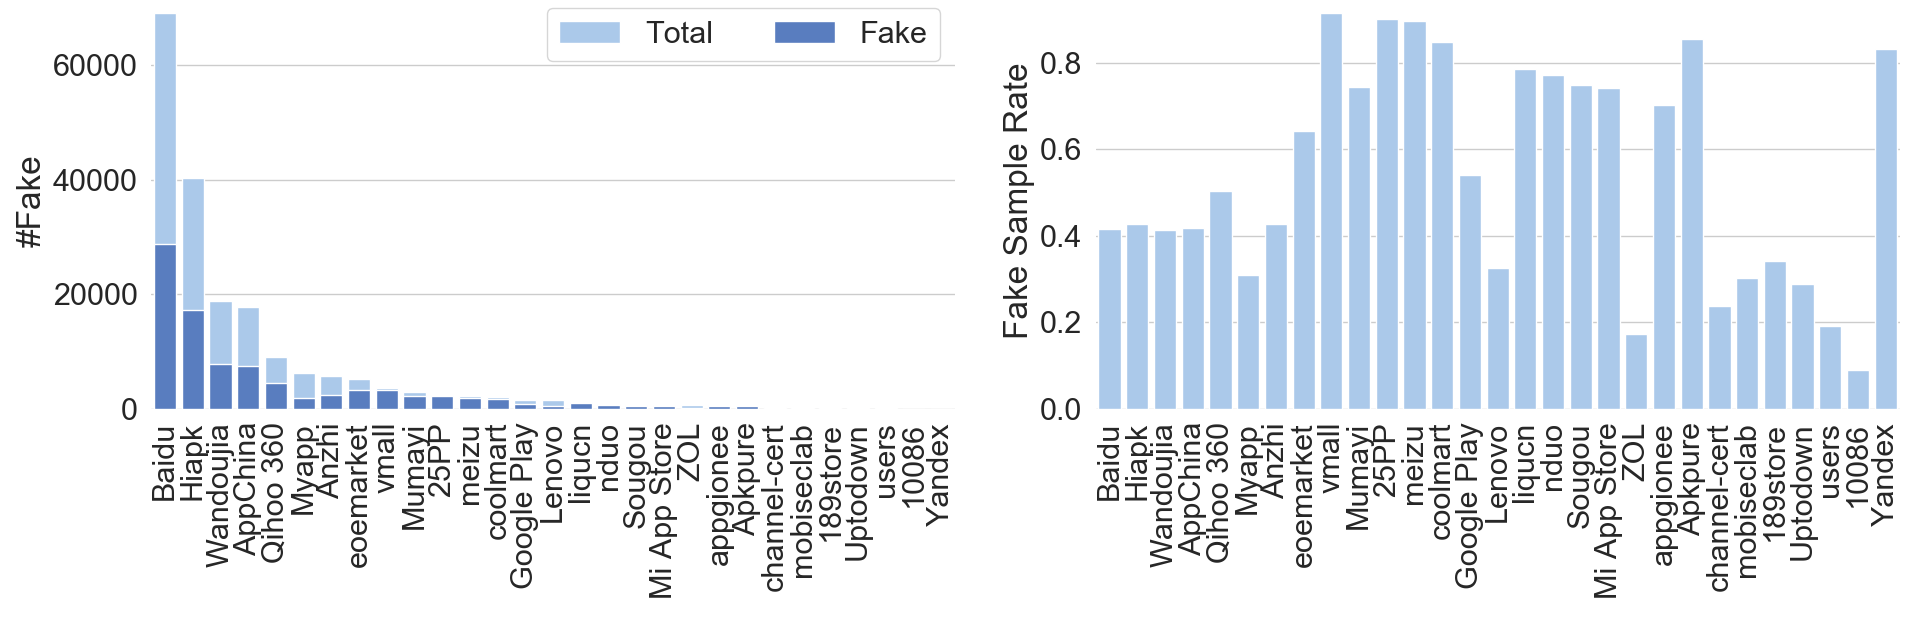
\includegraphics[width=\textwidth]{./Figures/edwin-Number_of_samples_collected_markets_3.png}
	\caption{从不同应用市场中收集到的应用数量以及各市场仿冒率}
	\label{fig:Sample_source}
\end{figure*}

\begin{Def}
    仿冒率

    某款App~$a$的仿冒率$fake~sample~rate_a$指与其关联的仿冒样本的数量$fake_a$与该App正版样本的数量$total_a$的商(\autoref{equ:fake_rate_app})。

    某应用市场$AS$的仿冒率$fake~sample~rate_{AS}$则是其中包含的所有目标App的均值(\autoref{equ:fake_rate_mkt})。
\end{Def}

\begin{equation}
    fake~sample~rate_a = \frac{fake_a}{total_a}
    \label{equ:fake_rate_app}
\end{equation}
\begin{equation}
    fake~sample~rate_{AS} = Avg(fake~sample~rate_a, \forall a \in \text{\{目标App\}})
    \label{equ:fake_rate_mkt}
\end{equation}
\vspace{0.5mm}

% Although both \texttt{Baidu App Store}~\cite{Baiduappstore} and \texttt{Hiapk}~\cite{Hiapk} hold a fake sample rate of about 40\%, the number of fake samples from \texttt{Baidu App Store} exceeds \texttt{Hiapk} to a great extent due to its dominant total sample number.
尽管\texttt{百度手机助手}~\cite{Baiduappstore}和\texttt{安卓市场}~\cite{Hiapk}的仿冒率均为40\%左右,在所有的31个渠道中处于中等水平,但由于源于这两个渠道的样本基数最大,所以从这两个应用市场搜集到的仿冒样本数也是最多的。

% Although no connection between the number of fake samples and market can be found from our data, we notice that the relationship between apps and markets may affect the fake rate.
图中数据显示,应用市场的样本数量和仿冒率并没有直接联系,但是我们仍然有一个有趣的发现,那就是App本身和市场的关系有可能是影响App仿冒率的一个因素。
% This is well supported by the low fake rate of \texttt{Myapp}~\cite{Myapp} -- the app market provided by \texttt{Tencent}, which is also the 12 out of 50 developers in our target apps.
\texttt{腾讯}旗下的应用市场\texttt{应用宝}~\cite{Myapp}中较低的仿冒率可以很好地为这个发现提供数据支持,因为我们的50款目标App中,有12款都是腾讯公司开发的应用。

\subsection{其他因素对仿冒样本数量的影响}
% Accordingly, we hypothesize the following factors may influence the number of fake samples of an app:
除了市场本身之外,我们还假设以下这些因素可能会影响某款App对应的仿冒样本数量:

% \noindent{\bf Hypo 2.2:} The number of fake apps are closely related to how popular an app is.
{\bf 假设 2.2}:仿冒应用的数量与其对应的正版App的受欢迎程度有密切联系。

% \noindent{\bf Hypo 2.3:} Update frequency effects the number of fake samples.
{\bf 假设 2.3}:应用的更新频率影响着其对应仿冒应用的数量。

% \noindent{\bf Hypo 2.4:} Category is a factor influencing the fake sample number.
{\bf 假设 2.4}:App类别是影响仿冒应用数量的因素之一。

与三个假设对应的是三个研究问题:

% \noindent{\bf RQ 2.2}: Does the popularity of an app affect the number of its fake samples?
{\bf RQ 2.2}:一个App受欢迎的程度会影响对其仿冒的应用数量吗?

% \noindent{\bf RQ 2.3}: Does an app's update frequency influence its fake sample's number?
{\bf RQ 2.3}:一个App的更新频率会影响对其仿冒的应用数量吗?

% \noindent{\bf RQ 2.4}: Is the number of fake samples related to the app's category?
{\bf RQ 2.4}:一个App所在类别会影响对其仿冒的应用数量吗?

对于这三个研究问题,我们使用了皮尔逊积矩相关系数(Pearson product-moment correlation coefficient,简称PPMCC)来衡量应用数量和问题对应的几个维度的关联性。

% \noindent{\bf Answer to RQ 2.2.}
{\bf RQ 2.2. 结果}
% Intuitively, the more popular an app is, the more possible it would get shammed, for fake developers would mislead users to download their apps to gain profits.
从直觉上看,某款App越受欢迎,仿冒应用开发者就越有动机对其仿冒,然后诱导用户下载仿冒版本以获取利润。

% Note that each app has different amount of samples (including official samples and fake samples), processing our measurement directly based on the number of fake samples is incorrect.
要注意的是,每款目标App都有不同的样本数(无论是官方的或是仿冒的),所以我们不能拿仿冒样本的数量直接作比较。
% To counteract this bias, each fake count should be regularize into a \textit{fake sample rate}, the rate of fake samples in all collected samples of an app.
为了消除偏差,我们应该将样本数量归一化,使用\autoref{equ:fake_rate_app}定义的仿冒率对每个目标App进行比较。
% Next, we employ a metric called \textit{Pearson product-moment correlation coefficient (PPMCC)} to reveal relativeness between an app's fake sample number and its popularity, which uses the regularized fake sample rates and monthly activeness indicators (MAI) obtained from Analysys~\cite{yiguanqianfan}.
接下来,我们使用了皮尔逊积矩相关系数来计算一款App被仿冒的严重程度与其热度是否具有相关性。
相关计算会使用上述的仿冒率和从易观千帆~\cite{yiguanqianfan}获取的App月度热度指数计算。

\begin{Def}
    皮尔逊积矩相关系数

    两个变量之间的皮尔逊相关系数定义为两个变量之间的协方差和标准差的商(\autoref{equ:PPMCC})。
\end{Def}
\begin{equation}
    p_x,_y = corr(X,Y)=\frac{cov(X,Y)}{\sigma_x\sigma_y}=\frac{E[(X-u_x)(Y-u_y)]}{\sigma_x\sigma_y}
    \label{equ:PPMCC}
\end{equation}
\vspace{0.5mm}

% This value ranges from -1 to 1, the closer the PPMCC value is to 0, the weaker correlation between the two factors is indicated.
\autoref{equ:PPMCC}的值域为$[-1, 1]$,该值越接近0,表示两个变量之间的相关关系越弱。
% Surprisingly, according to our data, the value of PPMCC between this two factors is 0.246, revealing that the fake sample number and an app's popularity only hold their relativeness on a weak level, which does not match our expectation.
出乎我们意料的是,根据我们的数据,这两个因子之间的相关系数只有0.246。
这表明仿冒应用的数量和App的热度在相关性上只处于较弱水平,和我们的预期并不符合。

% \noindent{\bf Answer to RQ 2.3.}
{\bf RQ 2.3. 结果}
% We assume the update frequency is related to the number of fake samples of an app, for updates can usually help keep a software from being attack.
我们猜想更新频率有可能会与App被仿冒的次数相关联,因为升级通常会有漏洞修复等举措,可以帮助App免受攻击。
% The higher the update frequency is, the safer an app is supposed to be.
所以我们一款App的更新频率越高,其安全性能应该就会越好。

% To estimate the average update frequency of our target apps, the time when an app's official sample was crawled and when its latest official samples were crawled is marked.
为了评估一款目标App的平均更新频率,我们标记了每个官方应用样本被发行时的时间,精确到日。
% The difference between them is then divided by the number of that app's existing version to obtain an update frequency, with unit day/version.
然后我们找到最新发布的那个样本和最早发布的那个样本,求出他们发行时间的差值的绝对值与版本数的商,即为平均更新频率(单位:天/版本)

% The result PPMCC value of 0.084 shows that the connection between an app's update frequency and its fake sample rate barely exists.
相关系数的计算结果表示,更新频率和仿冒数量之间的关联度只有0.084,意味着两者之间几乎没有关联。
% We attribute this result to two reasons:
我们认为这个结果可能由两个原因导致:

% (1) The high update frequency (10 days/version on average for apps in our dataset) indicates app developers may not fix security issues in per update, weakening the function of update frequency as a security indicator.
1)在我们的数据集中,每款App的平均更新间隔为10天/版本。
这个较高的更新频率表面开发者可能不会每次都在更新中修正安全性问题,从而削弱了更新频率作为安全性指标的功能。

% (2) A large portion of fake samples in our dataset are not derived from repackaging. To this end, fake developers can produce fakes regardless of how well the official apps are protected.
2)结合前文的结果,我们数据集中的大部分仿冒样本都不是重打包应用,而是仿冒应用开发者自行开发的。
因此,无论官方版本受到的保护程度如何,仿冒应用开发者都可以制造出对应的仿冒应用。

% \noindent{\bf Answer to RQ 2.4.}
{\bf RQ 2.4. 结果}
% Some categories are potentially more profitable than others.
某些App类别比其他类别更有可能带来收益。
% A report from the app marketing company LIFTOFF~\cite{LIFTOFF_report} forecasts gaming to be the next most billable area.
根据一份来自App营销机构LIFTOFF~\cite{LIFTOFF_report}的报告预测,在未来,\texttt{游戏}类有望成为带来最高收入的应用分类。

\begin{ThreePartTable}
\centering
\renewcommand{\arraystretch}{1.05}
\footnotesize
\setlength{\belowcaptionskip}{-5pt}
\vspace{1mm}
% \rowcolors{2}{gray!15}{white}
\begin{longtable}{l l c c c c c c}
\caption{目标App与其相关统计}\label{table:data-statistics}\\
\toprule
{\bf 应用名} & {\bf 类别} & \begin{tabular}[c]{@{}c@{}}{\bf 月度热} \\ {\bf 度指数} \end{tabular} & \begin{tabular}[c]{@{}c@{}}{\bf 更新频率} \\ {\bf (天/版本)} \end{tabular} & {\bf 样本总数} & \begin{tabular}[c]{@{}c@{}}{\bf 仿冒} \\ {\bf 样本数} \end{tabular} & {\bf 仿冒率} & \begin{tabular}[c]{@{}c@{}}{\bf 平均仿} \\ {\bf 冒延迟} \end{tabular} \\
\midrule
{\bf 微信}\tnote{*} & {\bf 社交网络} & {\bf 91.2K} & {\bf 6.4} & {\bf 9248} & {\bf 6447} & {\bf 69.7\%} & {\bf 12.1} \\
\rowcolor{gray!15} {\bf QQ}\tnote{*} & {\bf 社交网络} & {\bf 54.6K} & {\bf 10.7} & {\bf 11167} & {\bf 3780} & {\bf 33.8\%} & {\bf 9.2} \\
爱奇艺 & 视频 & 53.5K & 6.4 & 7586 & 3481 & 45.9\% & 9.3 \\
\rowcolor{gray!15} 支付宝 & 生活 & 48.1K & 10.2 & 983 & 231 & 23.5\% & 10.1 \\
{\bf 淘宝}\tnote{*} & {\bf 移动购物} & {\bf 47.5K} & {\bf 7.0} & {\bf 6003} & {\bf 3010} & {\bf 50.1\%} & {\bf 8.1} \\
\rowcolor{gray!15} 腾讯视频 & 视频 & 47.3K & 6.3 & 1429 & 68 & 4.8\% & 10.7 \\
优酷 & 视频 & 40.9K & 7.3 & 2058 & 262 & 12.7\% & 6.7 \\
{\bf 新浪微博}\tnote{*} & {\bf 社交网络} & {\bf 39.2K} & {\bf 5.3} & {\bf 5947} & {\bf 2715} & {\bf 45.7\%} & {\bf 5.7} \\
\rowcolor{gray!15} WiFi万能钥匙 & 系统工具 & 36.4K & 3.1 & 4808 & 2999 & 62.4\% & 3.0 \\
搜狗输入法 & 系统工具 & 33.3K & 11.0 & 898 & 40 & 4.5\% & 21.8 \\
\rowcolor{gray!15} 百度 & 资讯 & 32.4K & 11.1 & 15651 & 3514 & 22.5\% & 12.8 \\
腾讯新闻 & 资讯 & 28.7K & 8.5 & 1051 & 11 & 1.0\% & 8.9 \\
\rowcolor{gray!15} QQ浏览器 & 资讯 & 27.8K & 5.6 & 1369 & 43 & 3.1\% & 11.6 \\
今日头条 & 资讯 & 27.4K & 4.4 & 3538 & 179 & 5.1\% & 5.6 \\
\rowcolor{gray!15} 应用宝 & 应用市场 & 27K & 11.4 & 2419 & 266 & 11.0\% & 11.6 \\
快手 & 视频 & 24.4K & 3.2 & 8273 & 4270 & 51.6\% & 3.5 \\
\rowcolor{gray!15} 腾讯手机管家 & 系统工具 & 24.2K & 8.7 & 2463 & 1340 & 54.4\% & 8.7 \\
高德地图 & 生活 & 24K & 6.5 & 1225 & 51 & 4.2\% & 13.1 \\
\rowcolor{gray!15} 酷狗音乐 & 音乐 & 23K & 8.6 & 1313 & 122 & 9.3\% & 12.2 \\
QQ音乐 & 音乐 & 21.7K & 9.4 & 1132 & 65 & 5.7\% & 14.6 \\
\rowcolor{gray!15} 百度地图 & 生活 & 21.3K & 8.8 & 2609 & 1438 & 55.1\% & 15.3 \\
抖音 & 视频 & 19.4K & 11.1 & 317 & 12 & 3.8\% & 8.3 \\
\rowcolor{gray!15} {\bf 京东}\tnote{*} & {\bf 移动购物} & {\bf 18.5K} & {\bf 10.9} & {\bf 5000} & {\bf 2377} & {\bf 47.5\%} & {\bf 12.3} \\
UC浏览器 & 资讯 & 16.7K & 7.4 & 4232 & 1624 & 38.4\% & 7.0 \\
\rowcolor{gray!15} 360手机卫士 & 系统工具 & 15.4K & 12.4 & 3670 & 1423 & 38.8\% & 19.1 \\
全民K歌 & 音乐 & 14.7K & 21.1 & 618 & 215 & 34.8\% & 17.3 \\
\rowcolor{gray!15} 美团 & 生活 & 13K & 8.0 & 4752 & 1415 & 29.8\% & 6.9 \\
{\bf 拼多多}\tnote{*} & {\bf 移动购物} & {\bf 12.9K} & {\bf 6.6} & {\bf 2327} & {\bf 551} & {\bf 23.7\%} & {\bf 7.8} \\
\rowcolor{gray!15} {\bf 王者荣耀}\tnote{*} & {\bf 游戏} & {\bf 12.5K} & {\bf 15.5} & {\bf 2350} & {\bf 1319} & {\bf 56.1\%} & {\bf 12.3} \\
美图秀秀 & 摄影录像 & 12.4K & 5.4 & 1705 & 784 & 46.0\% & 5.8 \\
\rowcolor{gray!15} 火山小视频 & 视频 & 12.2K & 11.9 & 410 & 16 & 3.9\% & 9.6 \\
墨迹天气 & 生活 & 12K & 4.2 & 10081 & 7093 & 70.4\% & 4.7 \\
\rowcolor{gray!15} 滴滴出行 & 生活 & 11.8K & 8.6 & 943 & 117 & 12.4\% & 7.0 \\
华为应用市场 & 应用市场 & 11.8K & N/A & 0 & 0 & 0.0\% & N/A\\
\rowcolor{gray!15} {\bf 开心消消乐}\tnote{*} & {\bf 游戏} & {\bf 11.2K} & {\bf 19.7} & {\bf 2406} & {\bf 1738} & {\bf 72.2\%} & {\bf 20.6} \\
酷我音乐盒 & 音乐 & 11K & 2.9 & 3778 & 69 & 1.8\% & 4.2 \\
\rowcolor{gray!15} 西瓜视频 & 视频 & 11K & 11.5 & 866 & 100 & 11.5\% & 8.8 \\
OPPO应用商店 & 应用市场 & 10.8K & N/A & 0 & 0 & 0.0\% & N/A\\
\rowcolor{gray!15} 猎豹清理大师 & 系统工具 & 9.9K & 10.3 & 1803 & 388 & 21.5\% & 13.5 \\
360清理大师 & 系统工具 & 9.6K & 17.3 & 327 & 8 & 2.4\% & 8.5 \\
\rowcolor{gray!15} 360手机助手 & 应用市场 & 9.2K & 7.6 & 1616 & 137 & 8.5\% & 8.4 \\
WiFi管家 & 系统工具 & 8.8K & 19.5 & 1636 & 658 & 40.2\% & 15.7 \\
\rowcolor{gray!15} 讯飞输入法 & 系统工具 & 8.6K & 6.0 & 1451 & 8 & 0.6\% & 10.1 \\
百度手机助手 & 应用市场 & 8.2K & 11.4 & 3849 & 437 & 11.4\% & 14.5 \\
\rowcolor{gray!15} 小米应用市场 & 应用市场 & 7.8K & N/A & 0 & 0 & 0.0\% & N/A\\
{\bf WPS Office}\tnote{*} & {\bf 商务办公} & {\bf 7.4K} & {\bf 6.0} & {\bf 1152} & {\bf 69} & {\bf 6.0\%} & {\bf 7.8} \\
\rowcolor{gray!15} 美颜相机 & 摄影录像 & 7.1K & 5.3 & 1600 & 691 & 43.2\% & 6.3 \\
网易云音乐 & 音乐 & 7K & 10.5 & 616 & 6 & 1.0\% & 12.2 \\
\rowcolor{gray!15} 网易新闻 & 资讯 & 6.7K & 7.0 & 1441 & 93 & 6.5\% & 5.0 \\
{\bf QQ邮箱}\tnote{*} & {\bf 商务办公} & {\bf 6.6K} & {\bf 16.4} & {\bf 520} & {\bf 11} & {\bf 2.1\%} & {\bf 10.4} \\
\bottomrule
\end{longtable}
\vspace{-4mm}
\begin{tablenotes}
  % \item[*] Detailed descriptions are given in {\bf Answer to RQ 2.4}
  \item[*] 详情会在{\bf RQ 2.4. 结果}中给出
\end{tablenotes}
\end{ThreePartTable}

% Our 50 target apps are divided into 11 categories according to their functionalities, Table~\autoref{table:data-statistics} shows these categories and their corresponding fake sample rate.
根据应用功能划分,我们的50款目标App可以被分为11个类别。
\autoref{table:data-statistics}按每款App的热度排序,展示了每款App的类别和他们的仿冒率,同时还有他们的更新频率、关联样本总数等数据。
% In the same category, the difference between apps on fake rate lies in an acceptable range.
在相同的类别下,多数应用之间的仿冒率差值都位置在一个合适的水平。
% Without doubt, entertainment related categories like \texttt{游戏} and \texttt{Social Network} attract more fake samples.
毫无疑问地,娱乐向类别(比如\texttt{游戏}和\texttt{社交网络})吸引了更多仿冒应用开发者对其仿冒。
% Another field, \texttt{Online shopping}, has also gained special love from fake developers because online shopping is rapidly developing in China.
而另一个类别\texttt{移动购物}也特别受到了仿冒应用开发者的``关照'',因为移动购物在中国也正在快速地发展。
% Relatively, \texttt{商务办公} is not that attractive to fake developers, the average fake sample rate of this filed is only 4.05\%.
相对来说,商务方向的\texttt{商务办公}分类的应用就不是那么地吸引仿冒应用开发者了,这个领域下的App平均仿冒率只有4.05\%。
% Apps in these four categories are marked in bold in the table.
上述四个类别的应用都在表中被加粗标识,读者可以自行查阅。

% The result matches the observation in our daily life, people always tend to use mobile devices for entertainment instead of business purpose.
这个结果与我们在日常生活中观察到的结果相符,比起商务类用途,普罗大众更倾向于使用移动设备用作娱乐用途,消遣时间。
% It's pretty interesting to discover that the number of fake samples in a way reflects how people use their phone in their daily lives.
仿冒应用的数量从某种角度上反映了人们在日常生活中如何使用移动设备,这是个十分有趣的发现。

\vspace{5mm}
\noindent\fbox{
	\parbox{0.95\linewidth}{
		% \textbf{Remark 2}: As revealed by statistics, the number of samples returned from an app store does not imply a fake rate.
        \textbf{本节小结}: 正如由我们的统计和计算揭示的那样,从一个应用市场中能找到的应用样本数量并不能与应用商店的仿冒率相对应。
		% Additionally, the relationship between apps and market itself influences the number of fake samples from that market.
        此外,App本身与应用市场的关系也会影响到市场中对应App仿冒样本的数量。
		% To our surprise, an app's update frequency is not tightly correlated with its fake rate.
        出乎我们意料的是,App的更新频率并没有与仿冒率相关联。
		% We owe this to the fact that apps are updated too frequently and that repackaged samples are of minority in our dataset.
        我们认为这是由于应用更新频率太高、而且重打包应用在我们的数据集中占少数而导致的结果。
		% We further observe that ``category'' as a factor has greater influence on the number of fake samples of an app than ``popularity'' and ``update frequency''.
        我们进一步观测到,与\texttt{更新频率}和\texttt{应用热度}相比,\texttt{应用分类}这一因素对App的仿冒率有更大的影响。
	}
}

% \subsection{Developing Trend}
\section{仿冒应用的发展轨迹}
% In order to figure out fake apps' characteristics or behavior patterns over time, we propose the following research questions:
在这个视角下,我们希望结合时间维度,从我们的数据中挖掘信息。
随着时间推移,仿冒应用的特征和行为模式是否有发生改变?
这些年来,仿冒应用这个灰色产业是否有过变迁?
利用我们提取数据中的\emph{搜集时间}数据项,我们复原了各种不同的时间线以解答上述问题。

\subsection{仿冒应用的研发延迟}
在正版应用推出新版后,如果一个仿冒应用能在越短时间内推出对应的新版本,仿冒应用的开发者就越有可能蹭上软件更新的热度,从而获利。
对此,我们提出了以下研究问题:

% \noindent{\bf RQ 3.1} After a new version of an official app is published, how long do fake developers take to publish a new fake sample? In other words, how soon will these copycats appear?
{\bf RQ 3.1}:在一个官方应用的新版本推出之后,仿冒应用开发者需要花多少时间去推出对应版本的仿冒版?
换句话说,这些``山寨''版本会过多久出现?

在分别复原官方应用的更新时间线和对应仿冒版本的发布时间之后,我们得到了以下结果:

% \noindent{\bf Answer to RQ 3.1.}
{\bf RQ 3.1. 结果}
% We compute this latency and show its distribution in Fig.~\autoref{fig:Fake_latency_overall_distribution}.
我们计算出了每版App被仿冒的延迟时间和延迟的分布情况,结果显示在\autoref{fig:Fake_latency_overall_distribution}中。

\begin{figure}
	\centering
	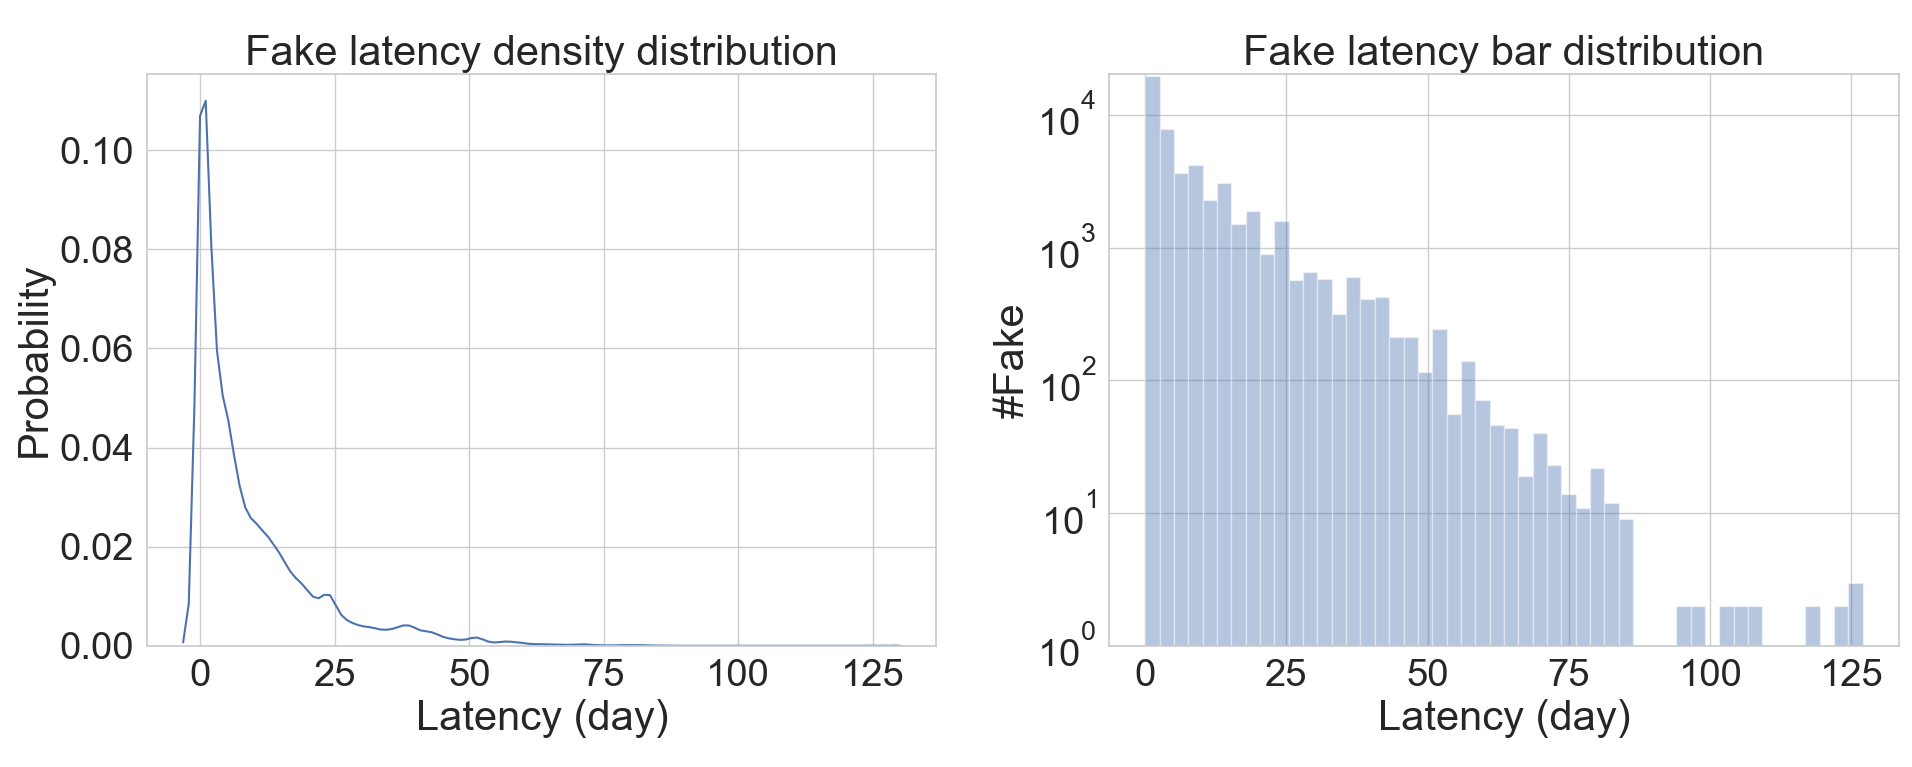
\includegraphics[width=\textwidth]{./Figures/edwin-Fake_latency_overall_distribution2.png}
	\caption{仿冒延迟总体分布}
	\label{fig:Fake_latency_overall_distribution}
\end{figure}

% Due to various reasons, it is hardly possible to retrieve the complete updating timeline for every single official app in our study, yet we approximately reproduce them with our data.
出于多种原因,我们很难为研究中的所有50款目标App回溯出它们每个版本更新的时间点,然而,我们凭借数据库中的数据大致地重现了他们的更新时间线。
% Firstly, we categorized all the official samples by their origins, and further categorized samples in each origin by version number.
首先,我们对所有收集到的官方样本按照他们的App源进行分类,然后再按照版本号对App源类下的所有样本分类。
举个例子,一开始是使用``爱奇艺''作为搜索源的所有官方样本都会被归回``爱奇艺''类下,然后再按版本号分类。
这么做的原因是,即使是官方渠道发布的版本,有些App在不同应用市场上架的时间和内容也会略微有差别,可能会导致一个版本的正版App有多个样本的结果。
这个做法就是为了消除上述情况带来的影响。
% After that, for each app and each version the samples are sorted by the date they were crawled, so by extracting the crawled date of the first sample in each version, we can obtain the earliest date a version is released.
之后,对于每款App和每个版本,我们都按照被爬取到的日期时间戳对对应的样本进行排序。
这样的话,通过提取每个版本中第一个版本被爬取的时间,我们就可以知道这个版本的官方App最早的发布日期了。
% Lastly, by combining and sorting the release dates of different versions according to different apps, we can reproduce the updating timelines of our target apps.
最后,将每款App中每个版本最早的发布日期串联起来,我们就可以大致重现每款App的更新时间线。

% To find out the release latency of a fake app, all the dates on the timeline of the corresponding official app are compared in order to find out the smallest negative difference which we define as the release latency.
由于仿冒样本大多不是重打包应用,我们没办法为每个仿冒样本精确匹配一个对应的正版版本,为了找到某个仿冒样本的仿冒延迟,我们会提取出它被爬取的日期时间戳,然后将这个时间戳与正版更新时间线上的所有版本进行对比,找到不晚于这个仿冒样本发布的最晚发布官方版本的发行时间,然后取他们的时间差作为仿冒延迟。
% Fig.~\autoref{fig:Fake_latency_overall_distribution} shows that most fake samples are published with the latency shorter than 20 days.
按照\autoref{fig:Fake_latency_overall_distribution}的结果,绝大多数仿冒样本在官方应用推出后的20天内就被发布了。
% According to our statistics, 60\% of fake samples show up in 6 days after a new version of the official app is published.
根据我们的统计,有60\%仿冒应用在正版App被推出的6天内就被发布出来了。
% This reveals a truth that fake developers are swift in action.
这表明仿冒开发者的行动十分迅速。

\subsection{仿冒应用安全证书的存活时长}
从某个角度看,仿冒应用安全证书的存活时长反映了应用市场的监管力度大小,也能反映市场之间在安全方面是否具有良好的合作机制。
所以我们有研究问题如下:

% \noindent{\bf RQ 3.2} How long can a fake app's certificate survive?
{\bf RQ 3.2}:一个仿冒应用开发者的安全证书可以存活多久?

我们整理了不同仿冒应用安全证书的出现时间,得出了下面的结果:

% \noindent{\bf Answer to RQ 3.2.} Fig.~\autoref{fig:Fake_certificate_survival_distribution} shows the distribution of the time a fake certificate can survive in markets.
{\bf RQ 3.2. 结果}\autoref{fig:Fake_certificate_survival_distribution}展示了不同仿冒应用安全证书在应用市场里存活时间的总体分布。
% In the left density distribution subplot, $x$-axes is the latency and $y$-axes shows the probability density of data at corresponding $x$ value.
在左边的密度分布函数图中,$x$轴表示其存活的时长,$y$轴则表示了与$x$轴上的值对应的概率密度。
% The total area under the curve is 1, and the area under two $y$ values $y1$ and $y2$ is the probability of their corresponding value $x1$ and $x2$ account for in data.
曲线下的总面积为1,任意两个$y$值$y_1$、$y_2$之间的曲线下面积是其对应的$x$轴上的值$x_1$、$x_2$在数据中占有的概率。
% For example, in Fig.~\autoref{fig:Fake_certificate_survival_distribution}, the area beneath curve between 0 to 200 on $x$-axes is close to 0.8, which means nearly 80\% of certificates only survive for no more than 200 days.
比如说,\autoref{fig:Fake_certificate_survival_distribution}中$x$轴从0到200之间的值对应的$y$轴曲线下方的区域面积接近0.8,意味着约80\%的仿冒应用安全证书不会存活多于200天。

% To judge how long a fake certificate can survive is similar to how we calculate the update frequency of an app, the first time and the last time a fake sample from the same certificate gets crawled are marked.
断定一个仿冒应用安全证书存活市场的方法和我们计算应用更新频率的方法稍有类似,我们会把某个安全证书关联的所有样本都找出来,提取出其中最早和最晚被爬取的样本的发布日期时间戳,然后将他们的差值的绝对值当作是这个安全证书的存活时长。
% The time when a sample was crawled from a market might be different from the time when it is available in the market, but our crawler downloads new samples from different markets by days and we also use days as the unit in our measurement, so we can approximately regard this two values as the same one.
从时长上爬取到样本的日期与样本在应用市场上实际能存活的时间稍有不同,但由于我们的爬虫工具每日都从应用市场中爬取样本,而我们又没有其他方法可以知晓某款App具体在应用市场中上架了多久,我们只能近似地将上述提到的时间差当作是某个安全证书能在应用市场上存活的时间了。

\begin{figure}[htbp]
	\centering
	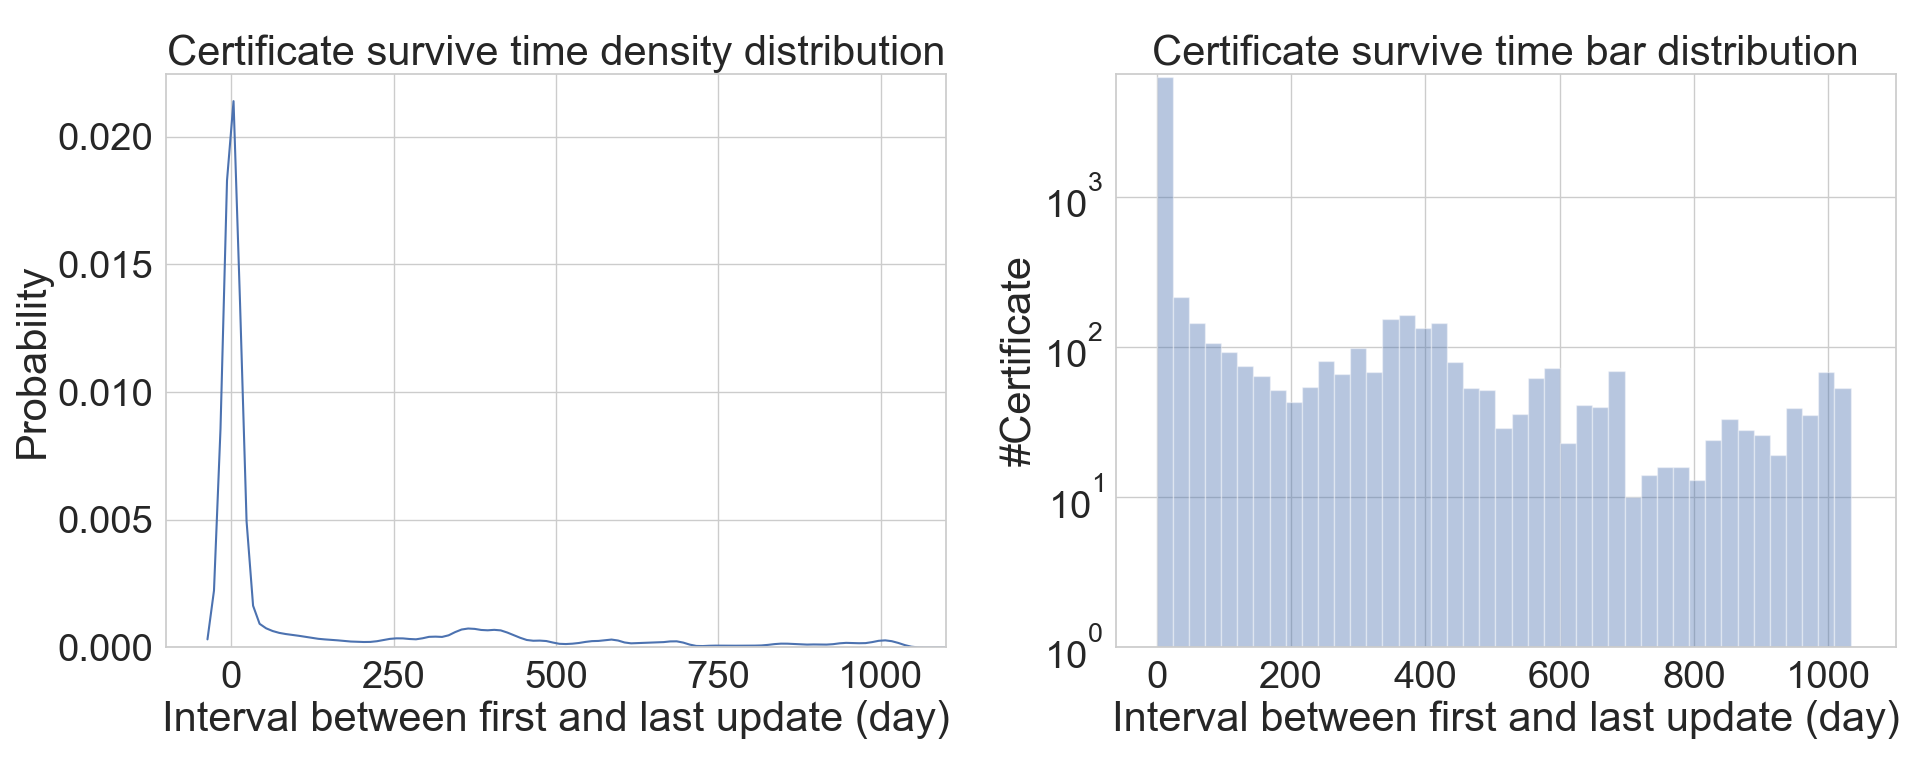
\includegraphics[width=\textwidth]{./Figures/edwin-Fake_certificate_survival_distribution2.png}
	\caption{仿冒应用安全证书存活时间分布}
	\label{fig:Fake_certificate_survival_distribution}
\end{figure}

% As shown in Fig.~\autoref{fig:Fake_certificate_survival_distribution}, the distribution of fake certificate survival time shows that almost all the fake certificates live a short life, which means most fake certificates only show up in a short period of time.
正如\autoref{fig:Fake_certificate_survival_distribution}所示,仿冒应用安全证书存活时间的分布表明几乎所有仿冒应用安全证书都只能存活相当短的时间,这表明大多仿冒应用只会在一个很小的时间窗口里出现,然后迅速消失。
% This can be explained by a scheme that most markets have.
这可以由大部分市场都有的一个安全机制解释。
% Once an app is found malicious or illegal, the market would stop that specific developer from uploading more samples by refusing to receive samples with the same certificate.
只要一款App被发现具有恶意行为或者违法行为,应用市场就会禁止开发者再使用该证书上传应用,也就是我们常见的封号处理。
% There are also a number of certificates which can survive for a long time.
但是,我们也能发现有一部分的仿冒应用安全证书存活了相当久的一段时间。
% According to the figure, some fake certificates even traverse the whole study interval.
根据图表信息,我们可以看到有的仿冒应用安全证书的生命周期甚至贯穿了我们整个研究截取的时间周期。
% We will conduct a case study on this phenomenon in Section ~\autoref{sec:casestudy}.
对于这个异常样本,我们会在\fullref{chp:casestudy}中有更详尽的案例分析。

\begin{figure}[htbp]
	\centering
	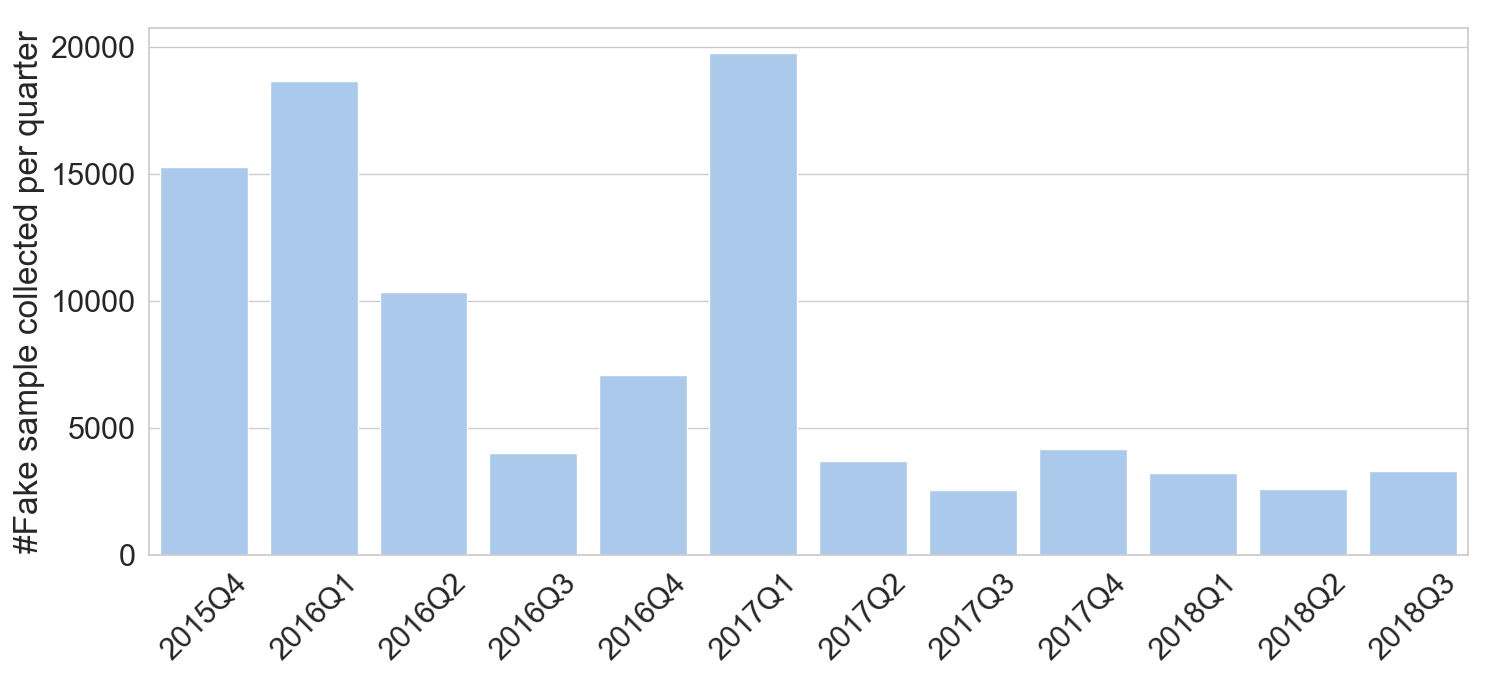
\includegraphics[width=\textwidth]{./Figures/edwin-Number_of_samples_collected_per_quarter_3.png}
	\caption{每季度爬取到的仿冒样本数量(2015年第四季度到2018年第三季度)}
	\label{fig:Number_per_quarter}
\end{figure}

\subsection{仿冒应用的行业变迁}
随着时间推移,仿冒应用这个灰色产业是否有过变迁?
我们对此提出了研究问题:

% \noindent{\bf RQ 3.3} Is there a changing pattern of fake samples over time?
{\bf RQ 3.3}:仿冒应用是否存在一个随着时间变化的模式?

我们统计了不同时间段所搜集到的样本数量,得出了结果如下:

% \noindent{\bf Answer to RQ 3.3.} Fig.~\autoref{fig:Number_per_quarter} shows the number of fake samples collected per quarter since the fourth quarter of 2015.
{\bf RQ 3.3. 结果}\autoref{fig:Number_per_quarter}呈现了我们的爬取工具自2015年第四季度起在每个季度爬取到的仿冒样本的总量。
% Although a large number of new fake samples get released in every quarter, the figure shows a tendency that the total number of fake apps on markets is gradually decreasing by years.
尽管我们每个季度都能爬取到新上架的大量仿冒样本,图表信息表明,市场上仿冒应用的总数正在呈现逐年减少的趋势。
% Note that our statistics only focus on fake samples, consequently this phenomenon does not indicate the underground industry is turning down.
要注意的是,我们的研究仅仅针对仿冒应用。
因此这个现象并不表明移动黑产的发展具有萧条的趋势。
% Instead, we suppose this is possibly caused by the reform of fake apps.
相反地,我们认为这个现象更有可能是由黑产内部改革而导致的。

% On one hand, as stricter review schemes and stronger protection systems are applied on app stores, it's inevitable that fake apps in this study, become harder and harder to get on the shelf.
从一方面看,随着信息技术发展,应用市场逐渐配备上了更智能、严格而又强大的监管机制和安全系统,本研究中的仿冒应用开发者无疑更难以将仿冒的应用投放到市场上了。
% On the other hand, the new generation of malicious software, such as ransomware~\cite{ransomware} is impacting the underground industry.
从另一方面看,新一代的恶意软件,比如WannaCry等勒索软件~\cite{ransomware}也正在影响着整个黑产工业。
% Compare to fake apps, the new malicious apps are not only hard to defend (due to the innovative or even state-of-the-art techniques they utilize) but also extremely profitable.
与仿冒应用相比,这些新一代的恶意软件不仅更难以防范(传统的反病毒软件思路是提取已有恶意代码的特征,从而识别恶意行为,但这无法遏制新型的恶意行为),而且也似乎更容易能获取暴利。
% Wannacry, a ransomware which was first spotted in the 2nd quarter of 2017, conquered tens of thousands of devices in a couple of weeks, which directly pulled up Bitcoin's price like a rocket~\cite{wannacry_bitcoin_news}.
Wannacry作为一种新型恶意软件,自2017年第二季度被首次发现开始,就能在数周内攻克数以千万计的设备,并让比特币的价格像搭火箭一样直线飙升~\cite{wannacry_bitcoin_news}。
% Afterward, in the first quarter of 2018, a burst of cryptomining malware on phones emerged~\cite{comodo_report}.
之后不久,在2018年的第一季度,移动设备上也爆发了一系列的加密采矿恶意软件~\cite{comodo_report}。
% This may be the reason why the number of fake samples suffers two suddenly drops in the second quarter of 2017 and the first quarter of 2018, respectively.
所以我们有理由猜测2017年第二季度和2018年第一季度的仿冒应用上架数量下跌是受到了新形态黑产的冲击。
当然,要去证明这个猜想还需要采集更多数据、进行更深入的研究,并不在本文的讨论范围之内,我们可将这个疑问放入\fullref{chp:future}展望与未来工作中。

\vspace{5mm}
\noindent\fbox{
	\parbox{0.95\linewidth}{
		% \textbf{Remark 3}: Fake apps can be produced in a relatively short time, and the dropping number of fake samples by years suggests that they are mired in recession.
        \textbf{本节小结}:仿冒应用可以在极短时间内被研发并上架,而仿冒样本逐年下降的新增量,也许表明了仿冒应用产业正在陷入衰退期。
		% Besides, only a few fake certificates survive for a long time, confirming that markets' protection schemes do work to some extent.
        此外,只有很小一部分的仿冒应用安全证书可以存活很长的一段时间,这表明应用市场的保护监管机制在一定程度上的确能发挥作用。
	}
}

\section{本章小结}
本章分别从\emph{仿冒应用的基本特征}、\emph{针对仿冒样本的量化分析}和\emph{仿冒应用的发展轨迹}三个不同视角对采集到的数据进行了分析,并在每个视角后的本节小结中概括了每个视角的结论。
在下一章,我们将会从数据中挑选出一些较有代表性的真实数据,印证我们在本章中的发现,同时为上述发现提供有力的事实依据。

\clearPaperPage

\chapter{仿冒应用的评论分析}
\label{chp:feedback}

应用市场中的用户反馈区是Android应用生态的重要部分,也是移动黑灰产从业者的深耕之地。
热心用户会在评论区提出反馈,黑灰产从业者则会利用排名欺诈的手段牟取利益。
为了进一步对仿冒应用的生态有所了解,笔者有必要搜集和分析仿冒应用的评论。
对于与仿冒应用相关的评论,有以下待解答的问题:
有多少用户会对这些应用进行评论?
用户对这些应用的使用感受如何?
仿冒应用是否会跟排名欺诈有所联系?

为了回答这些问题,笔者从\texttt{360手机助手}应用商店中爬取了部分应用和它们的所有历史评论,然后对这些评论进行了处理和分析。

\section{仿冒评论数据收集}
由于Janus平台上并不提供评论数据,\mytool 的爬虫模块也只支持应用爬取,所以笔者另外在应用市场上重新收集了评论数据。
在\texttt{360手机助手}应用商店中,笔者随机挑选了856个应用,爬取了这些应用的APK包和对应的所有历史评论。
之后,笔者将上一次数据收集时保存的正版应用的信息重新导入\mytool,从新收集的应用中筛选出了对应仿冒应用。

每条评论都会附带一个评价分数,某款App在市场上的平均评价就是所有评论评分的均值。
对于每条评论信息,笔者能收集到的数据项是:\texttt{应用包名}、\texttt{用户ID}、\texttt{评论内容}、\texttt{评分}和\texttt{评论日期}共五项。

\subsection{评论数据概览}
在笔者收集评论的所有856个应用中,有6款应用与先前仿冒应用数据中的包名对应。
要注意的是,由于本研究的仿冒应用列表为针对50个热度最高的目标App整理而成,而收集评论的应用是在整个市场范围内随机挑选的,所以这里的仿冒应用占总体应用比例较小。但这不意味着整个市场中就只有这几款应用是仿冒应用。
另外,由于这856个应用是随机挑选的,笔者认为这批数据具有一定的代表性,可以应以反映整个市场的评论分布情况。
本次研究一共爬取到了267,397名用户的365,461条评论,其中6款仿冒应用的所有历史评论共计3,591条,来自2,946名用户。

\subsection{基础分析}

% 画图用的python代码
% font_size = 20
% sns.set(style="white")
% fig = plt.figure()
% plt.xticks(fontsize=20)
%
% ax1 = fig.add_subplot(111)
% bar = sns.barplot(x="Package name", y="Comment cnt", data=df, ax=ax1, palette="Blues_r")
% ax1.tick_params(axis='y', labelcolor=“tab:blue”)
% plt.yticks(fontsize=font_size)
% ax1.set_ylabel("# Comments", color="tab:blue", size=font_size)
%
% ax2 = ax1.twinx()
% line = sns.lineplot(x="Package name", y="Rating", data=df, ax=ax2, c="r", linewidth=3)
% ax2.tick_params(axis='y', labelcolor=“tab:red”)
% ax2.set_ylabel("Rating", color="tab:red", size=font_size)
% plt.yticks(fontsize=font_size)
% # 折线图y轴范围
% plt.setp(line, yticks=[4, 4.2, 4.4, 4.6, 4.8])
% # 旋转x轴标签
% for axis in [ax1, ax2]:
%     for tick in axis.get_xticklabels():
%         tick.set_rotation(10)
%
% # 清除上方右方边框
% sns.despine()
% plt.show()

\begin{figure}[htbp]
	\centering
	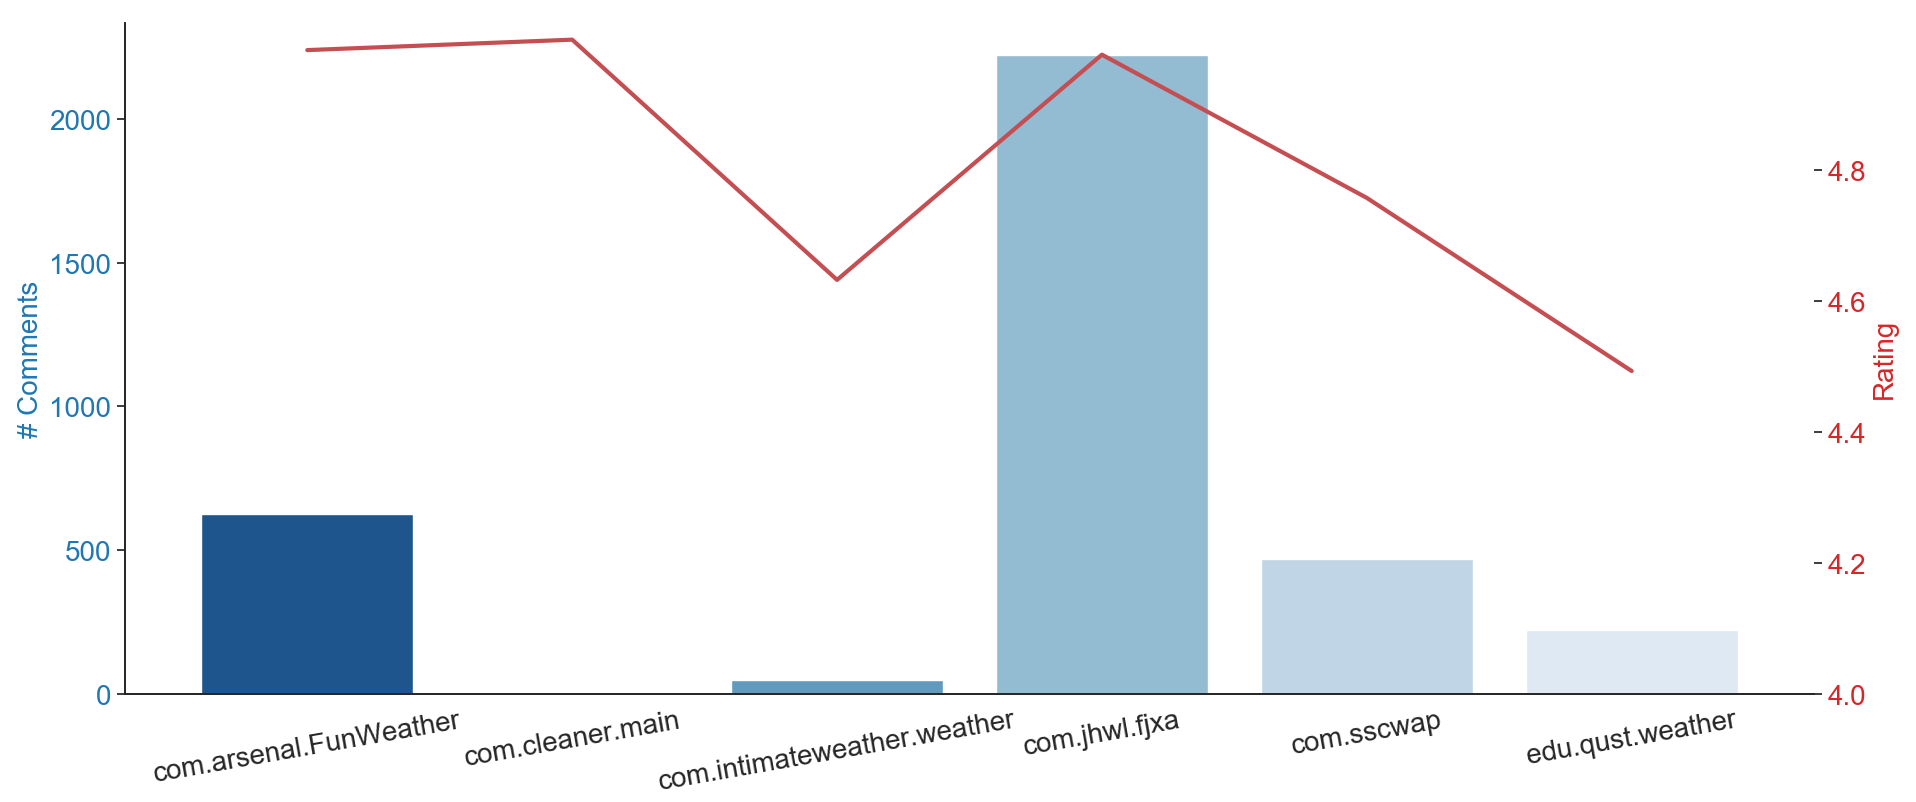
\includegraphics[width=\textwidth]{./Figures/edwin-cmt-ratings-dist-3.png}
    \caption{各仿冒应用在\texttt{360手机助手}商店中的评论数量与评分分布}
    \label{fig:cmt_dist_fake}
\end{figure}

\autoref{fig:cmt_dist_fake}显示了6款应用收到的评论数量和评分分布。
蓝色的柱状图表示评论数量,红色的折线图表示各评论汇总后的平均评分(以5分为满分算),$x$轴分别代表不同样本的包名。
按评论数从多到少的顺序看,\emph{com.jhwl.fjxa}收到了2223条评论,平均评价为4.98分;
\emph{com.arsenal.FunWeather}收到了626条评论,平均评价也是4.98分;
\emph{com.sscwap}收到了467条评论,平均评价4.76分;
\emph{edu.qust.weather}收到了223条评论,平均评价4.49;
\emph{com.intimateweather.weather}和\emph{com.cleaner.main}分别只收到了49条和3条评论,而他们的平均评价则分别为4.63分和5分。
乍眼一看,上述应用的评分都十分高。
以下是一些热门应用的评分和这些仿冒应用的评分的对比:
在同一市场下,移动购物类应用\texttt{淘宝}的评分为4.55分,近年十分受欢迎的短视频应用\texttt{抖音}平均评价是4.5分,游戏类应用\texttt{开心消消乐}的评分是3.65分,而\texttt{微信}的平均评价更是只有3.45分。
上述应用毫无疑问都是十分优质的App,庞大的用户基数带来的大量真实评价会使得平均评价较为稳定,不会因为在短时间内收到少量好评或者差评就产生较大的评价波动。
在\texttt{淘宝}等应用作为基准的情况下,6款仿冒应用的评分之高不禁令笔者想到恶意刷评的相关研究。
然而,笔者不能仅凭几个应用的平均评价对比就咬定仿冒应用存在刷好评的行为。
因此,本文先分析数据集的整体分布,再作进一步比较。

在不考虑上述提到的恶意刷评的情况下,一款应用的使用人数越多,就越有可能收到来自用户的评价。
所以可以在一定程度上,从一款应用的评论数目估计其用户数量的多少。
\autoref{fig:cmt_dist_total}中的两个小提琴图显示了所有856个应用收到评论的数量和总体评级分布,有助于了解市场中应用的热度分布情况和用户的评价倾向。

% Python 作图代码
% font_size = 20
% sns.set(style="whitegrid")
% fig = plt.figure()
%
% ax1 = fig.add_subplot(121)
% bar = sns.violinplot(x=df2["Cmt cnt"], ax=ax1)
% ax1.set_xlabel("Package #Comment Distribution", size=20)
% plt.xticks(size=20)
%
% ax2 = fig.add_subplot(122)
% line = sns.violinplot(x=df2["Pkg Rating"], ax=ax2)
% ax2.set_xlabel("Package Rating Distribution", size=20)
% plt.xticks(size=20)
%
% # 清除上方右方边框
% sns.despine()
% plt.show()

\begin{figure}[htbp]
	\centering
	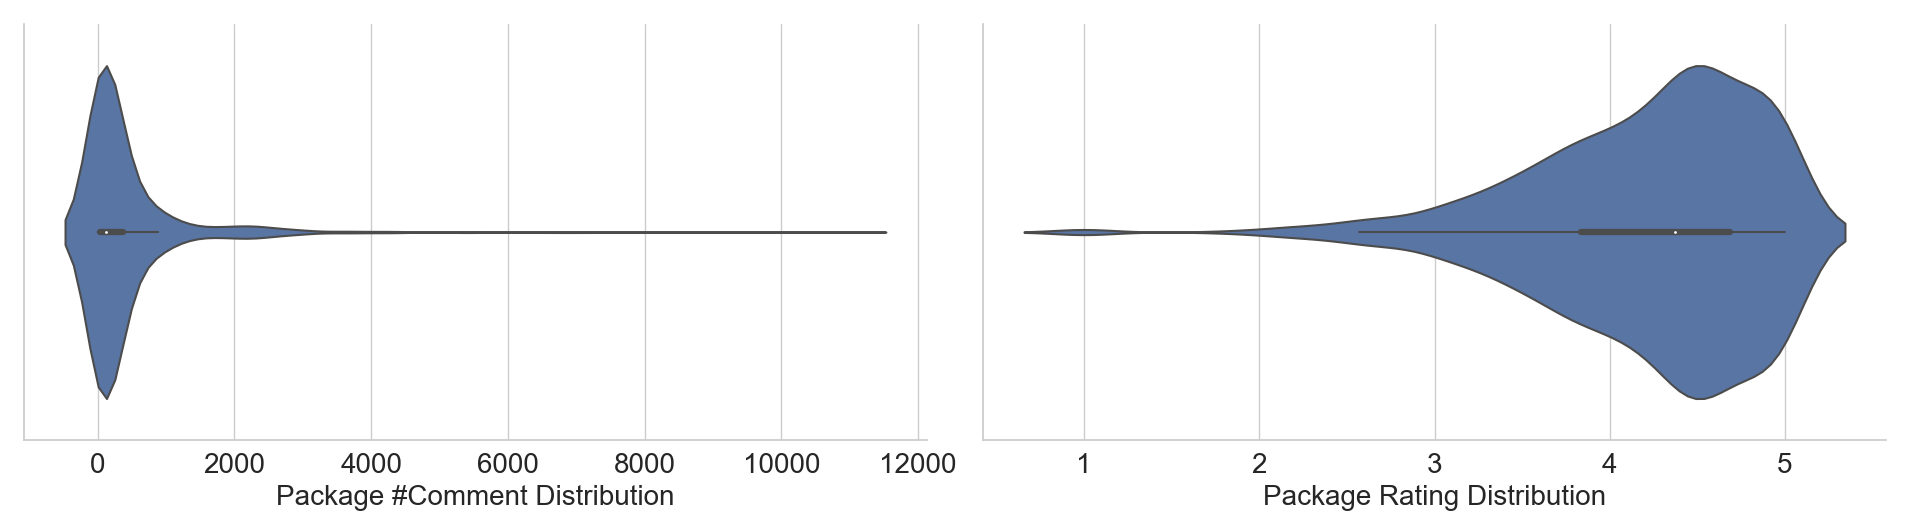
\includegraphics[width=\textwidth]{./Figures/edwin-360-comment-dist.png}
    \caption{所有856个应用在商店中的评论数量与评分分布}
    \label{fig:cmt_dist_total}
\end{figure}

左边的小提琴图表示每个应用收到的评论总数分布,其四分位数分别为31, 124和375.75。
这说明,在收集到的856个应用中,25\%的应用收到小于或者等于31条评论,50\%的应用收到小于或等于124条评论。
如果某款应用收到的评论数大于375条,那这款应用的评论总数就能排在前25\%了。
另外,数据显示,仅有5\%的应用收到了超过2,109条评论。
结合仿冒样本的数据,\emph{com.jhwl.fjxa}、\emph{com.arsenal.FunWeather}和\emph{com.sscwap}的评论数量都排在了前25\%,\emph{com.jhwl.fjxa}更是能排在前5\%的位置。
从数据上看,上面三款App相当受欢迎。

右边的小提琴图则表示各个应用收到的平均评价的分布情况,其四分位数分别为3.84,4.37和4.69,约5\%的应用平均评价为5分满分。
这个分布说明这个应用市场上的用户十分倾向于给出高分评价,至少有过半数的评论都是满分好评。
回到仿冒样本的数据,其中有两款评论少于100条,很可能存在较大的个体偏差,在此先忽略不计。
余下四款仿冒应用中也有三款的平均评价排进了前25\%,恰好也是评论数较多的\emph{com.jhwl.fjxa}、\emph{com.arsenal.FunWeather}和\emph{com.sscwap}。

结合两个维度的分布结果,\emph{com.jhwl.fjxa}、\emph{com.arsenal.FunWeather}、\emph{com.sscwap}三款App不仅用户众多,而且还好评如潮。
再回望\texttt{淘宝}、\texttt{微信}等应用的评分,两者之间似乎有了矛盾。
一款应用的用户越多,真实的评论数目越大,该款应用的评分就会趋向客观,直到收敛到一个可以反映应用质量的真实水平。
\emph{com.jhwl.fjxa}、\emph{com.arsenal.FunWeather}、\emph{com.sscwap}三款应用的用户量固然不能和\texttt{微信}、\texttt{淘宝}相比,但成百上千的评论数也暗示着一个不小的用户群体。
在用户群体有一定规模的情况下,还能保持名列前茅的平均评价,究竟是这三款仿冒应用的确受到了用户的热捧,还是另有原因?

\section{仿冒应用与排名欺诈关联验证}

\subsection{排名欺诈检测初探}

带着上述的疑问,笔者决定用自动化的方法试图寻找这几款应用是否有排名欺诈的可能。

\texttt{FRAUDAR}~\cite{hooi2016fraudar}是Bryan Hooi在2016年推出的一个算法,可以使用二分图挖掘的方法找出可能的虚假好评,并输出最可能涉及排名欺诈的应用和用户。
算法基于的假设是,普通用户的行为(在本文中即为对App评论的行为)是大致随机的,而用于进行排名欺诈的用户群的行为却会有比较明显的指向性(即针对购买了排名欺诈服务的App发送好评),而且为了将平均评分拉高,就意味着需要发送大量好评。
如果将用户和App分别看做两种不同节点,每条好评看作是两种节点之间的边,那么在这张用户-评论-应用图中,排名欺诈用户和对应的App之间就会有特别紧密的联系。
如果能把这个联系特别紧密的子图找到,就有可能从中找到真实的排名欺诈用户和应用。

由于此处的排名欺诈指用大量虚假好评刷高应用的平均评价,所以在寻找排名欺诈用户和对应应用时,应该只采用满分好评作为数据。
因此,本研究从所有评论中筛选出了满分好评,其总数为381,507条,由229,100名用户给出,分布于848个应用中,占评论总数的87.15\%。
笔者将\texttt{FRAUDAR}应用在了本研究的好评数据集上,找到了115名可疑用户和13个可疑应用。
经过比对后,笔者发现,13个可疑应用并不包含仿冒样本,而仿冒应用的所有评论条目中也没有源于那115名可疑用户的评论。
但\emph{com.jhwl.fjxa}的评价表现依然令人生疑,因此,笔者决定使用其他办法检测这几款仿冒应用的评论中是否存在排名欺诈的可能性。
基于本工作中现有的数据项,进行检测的角度可以分为两个,一个是评论用户可信度,另一个则是评论内容相似度。

\subsection{基于评论用户可信度的排名欺诈排查}

Mohammad-Ali~\cite{abbasi2013measuring}在2013年提出了一个个体行为相似度的计算方法。
在该算法中,用户行为相似度由\autoref{equ:usr_cre1}计算,如果相似度超过了某个阈值$T_1$,就可以将两名用户聚入同一类。
\autoref{equ:usr_cre1}中的$B(u_i, t)$指用户$u_i$在时间节点$t$的行为(在此处可以理解为对某一个应用给好评),而$\sigma(B(u_i, t), B(u_j, t))$则是一个用来计算用户$u_i$和$u_j$在时间为$t$时行为相似度的方程,Mohammad在文中选用的是\autoref{equ:usr_cre2}所示的Jaccard相似系数,所以本文在这里也选用了同样的Jaccard系数计算。

\begin{equation}
Sim(u_i, u_j) = \frac{1}{t_n - t_0}\sum_{t=t_0}^{t_n}\sigma(B(u_i, t), B(u_j, t))
\label{equ:usr_cre1}
\end{equation}
\begin{equation}
Jaccard(set_i, set_j) = \frac{|set_i \cap set_j|}{|set_i \cup set_j|}
\label{equ:usr_cre2}
\end{equation}
\vspace{0.5mm}

在这种计算方式下,那些仅给过一次好评的用户将会很容易成为噪声数据,对研究的结果产生影响,所以笔者先剔除掉了这部分数据。
仅给过一次好评的用户共186,775人,占所有给出好评用户的81.53\%。

在将行为相似的用户聚类之后,可以通过计算某一应用评论中疑似排名欺诈评论的占比、或是评论该App的可疑用户占所有可疑用户的占比来排查可能购买了排名欺诈服务的App。

\begin{Def}
	应用的用户可信度权重

	假设所有市场用户的集合为$G_{all}$,已知疑似排名欺诈用户群体$G_r$,用户以$u$表示,由任意用户$u_i$发布的评论$cmt_j$表示为$u_i \rightarrow cmt_j$,市场中的某一应用$app_k$的评论列表为$CL_{app_k}$。
	则该应用$app_k$的用户可信度权重$W_{app_k}$可由\autoref{equ:usr_cre3}中的二元组表示:
\end{Def}

\begin{equation}
	W_{app_k} = (w_{app_k}^0, ~w_{app_k}^1)
	\label{equ:usr_cre3}
\end{equation}
\begin{equation}
	w_{app_k}^0 ~ = ~ \frac{|\{u_i~|~u_i \in G_r, cmt_j \rightarrow u_i, cmt_j \in CL_{app_k}\}|}{|G_r|}
	\label{equ:usr_cre4}
\end{equation}
\begin{equation}
	w_{app_k}^1 ~ = ~ \frac{|\{cmt_j~|~cmt_j \in CL_{app_k}, cmt_j \rightarrow u_i, u_i \in G_r\}|}{|CL_{app_k}|}
	\label{equ:usr_cre5}
\end{equation}
\vspace{0.5mm}

在计算完权重之后,可以分别按其中的两个子权重对应用进行排名,筛选出可能购买了排名欺诈服务的App。

笔者分别将$T_1$设置为0.4,0.6和0.8,尝试对可疑用户进行聚类,结果分别将42,325名给出好评次数大于1的用户分到了10,024,14,520,15,493个聚类中。
可对这些聚类进行简单分析如下:
绝大多数聚类中都只有一名用户,即使是在相似度阈值只有0.4的情况下,也只有约7\%的聚类中包含3个或以上的用户(阈值为0.6和0.8时,该比例均为6\%)。
但是,当挑出包含用户数目大于10的聚类($T_1$为0.4/0.6/0.8时,这些聚类的占比分别为0.97\%/0.70\%/0.57\%)时,笔者却发现这些聚类分别包含了29,168/23,742/22,218个用户,他们所发布的好评共计分别有98,226/80,492/73,422条。
因此笔者推定,有一部分用户的行为模式相当近似且可疑,本文将会把这部分用户组成的群体看作是疑似的排名欺诈用户群体($G_r$)。

接下来,笔者分别计算了不同$T_1$下,三款仿冒应用在\autoref{equ:usr_cre4}和\autoref{equ:usr_cre5}中的两个权重,即三款应用中的好评用户占可疑用户的比例、以及其好评占所有可疑用户发布的好评的比例。
对于本章研究的三个仿冒应用,其两个子权重的结果分别展示在\autoref{table:usr-cred-res-1}和\autoref{table:usr-cred-res-2}中。

\begin{table}[htbp]
	\renewcommand{\arraystretch}{1}
	\small
	\centering
	\caption{各应用用户可信度权重及对应排名(一)}
	\vspace{1mm}
	\begin{tabular}{lcccccc}
		\toprule
		包名 & $w^0$($T_1$=0.4) & 排名 & $w^0$($T_1$=0.6) & 排名 & $w^0$($T_1$=0.8) & 排名 \\
		\midrule
		com.arsenal.FunWeather & 0.97 & 2 & 0.9 & 6 & 0.82 & 9 \\
		\rowcolor{gray!15} com.jhwl.fjxa & 0.85 & 15 & 0.84 & 12 & 0.8 & 12 \\
		com.sscwap & 0.02 & 303 & 5$\times10^{-3}$ & 346 & 5$\times10^{-3}$ & 318 \\
		\bottomrule
	\end{tabular}
	\label{table:usr-cred-res-1}
\end{table}

\begin{table}[htbp]
	\renewcommand{\arraystretch}{1}
	\small
	\centering
	\caption{各应用用户可信度权重及对应排名(二)}
	\vspace{1mm}
	\begin{tabular}{lcccccc}
		\toprule
		包名 & $w^1$($T_1$=0.4) & 排名 & $w^1$($T_1$=0.6) & 排名 & $w^1$($T_1$=0.8) & 排名 \\
		\midrule
		com.jhwl.fjxa & 0.05 & 11 & 0.06 & 10 & 0.07 & 11 \\
		\rowcolor{gray!15} com.arsenal.FunWeather & 0.02 & 45 & 0.02 & 39 & 0.02 & 39 \\
		com.sscwap & 2$\times10^{-4}$ & 261 & 8$\times10^{-5}$ & 279 & 9$\times10^{-5}$ & 251 \\
		\bottomrule
	\end{tabular}
	\label{table:usr-cred-res-2}
\end{table}

表中结果显示,无论是用哪种权重对应用可疑度进行排名,\emph{com.arsenal.FunWeather}和\emph{com.jhwl.fjxa}在总计的848个应用中都排在相当靠前的位置,所以这两个应用都相当可疑,十分可能具有排名欺诈行为。
另一方面,\emph{com.sscwap}的排名相对靠后,具有排名欺诈行为的可能性较小。

本组实验使用了服务器承担运算任务,实验服务器搭载了两颗Intel的至强E5-2367 V4版8核CPU,内存为252GB。
在$T_1$分别设置为0.4/0.6/0.8时,三组基于用户可信度实验用的python代码分别需要运行7,086/6,935/6,801分钟才得出结果。

\subsection{基于评论内容相似度的排名欺诈排查}
与前面的用户可信度计算相比,利用评论内容相似度排查排名欺诈的方法要相对简单一些,计算量也明显较小。
根据笔者的经验,在排名欺诈相关的评论通常具有很高的相似性,甚至一模一样,导致那些购买排名欺诈服务的应用中有很多相似甚至相同的评论。
所以,可以通过计算应用内相似评论的比率以筛选可能购买了排名欺诈服务的应用。

\begin{Def}
	应用评论重合率

	对于市场中的某一个评论列表为$CL_{app_k}$的应用$app_k$,假设其所有评论可以被分成$n$个组$CG_i (0 <i < n)$,则笔者定义该应用的评论重合率$RD_{app_k}$如下。重合率越高,应用越有可能存在排名欺诈行为。
\end{Def}

\begin{equation}
	RD_{app_k} = 1 - \frac{\sum_{i=0}^n|CG_i|}{|CL_{app_k}|}
	\label{equ:cmt_simi1}
\end{equation}
\vspace{0.5mm}

为了找出内容高度重合的评论,研究者可以用NLP中的词袋模型(Bag-of-words Model)将每个评论转化成一串词语列表。
具体做法是,先对每条评论进行分词,形成词袋,再用一种合适的标准去衡量不同词袋之间的相似度,并将相似内容聚为一类。
分词方面,本研究使用了中文分词项目“结巴”中文分词~\footnote{\url{https://github.com/fxsjy/jieba}},为了更好地从词袋中提取语义信息,本文还从网上整理了一份停用词(Stop words)表,在分词之后筛去停用词,以减少不含语义的停用词对相似度计算造成的干扰。
词频太低的词语也可能会对聚类产生影响,为此,本研究会在聚类前从各个词袋中删除总词频太低的词语。
而在衡量词袋相似度方面,本文再次使用了\autoref{equ:usr_cre2}的Jaccard相关系数。

另外,本研究要筛查的是排名欺诈行为,其本质是通过提供大量虚假好评提高应用的平均评价,所以还要从数据集中除去一部分评论较少的应用,因为他们不太可能购买了排名欺诈服务。
本文分别从数据集中剔去了总评论少于50条和总评论少于100条的应用,使得数据组中分别剩下511和455个应用参与排名。

在预处理过程中,本研究剔除了在所有评论中出现次数小于等于2的词语,然后以0.8为相似度阈值对评论进行聚类。

结果可见\autoref{fig:cmt_simi},其中图例上标注的``50''和``100''分别表示剔除了总评论少于50条的应用的数据组和剔除了总评论少于50条的应用的数据组,两个图形中的三条虚线分别是两组数据中的3个四分位数线。
``50''数据组的三条四分位数线分别对应$x$轴上0.09,0.17和0.30的位置,说明数据组中有25\%的应用评论重合率小于9\%,50\%应用的评论重合率小于17\%,如果某应用的评论重合率大于30\%,那么该应用的评论重合率就排在数据集的前25\%了。
与之类似,``100''数据组的三条四分位数线分别对应$x$轴上0.10,0.18和0.32的位置,表明两组数据整体的评论重合率并不高。
此外,``100''组的数据分布比``50''组的数据分布稍微偏向$x$轴右侧,证明接收到评论较少的应用的评论重合率的确也偏低。

\begin{figure}[htbp]
	\centering
	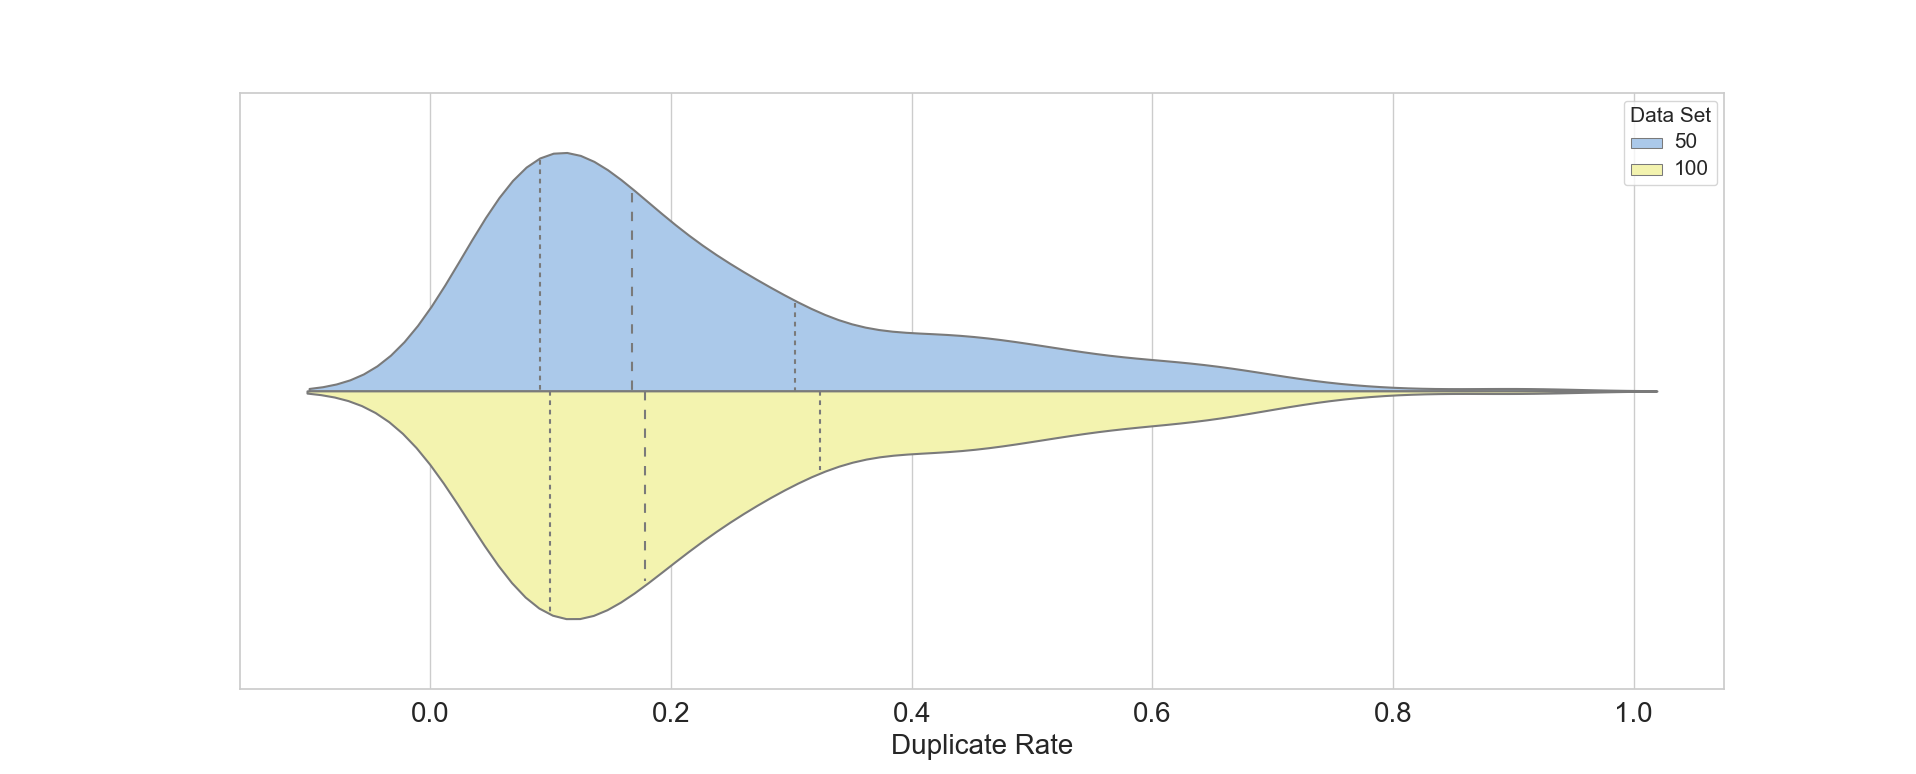
\includegraphics[width=\textwidth]{./Figures/edwin-cmt-simi-dist.png}
    \caption{两种数据组的应用评论重合率结果}
    \label{fig:cmt_simi}
\end{figure}

\begin{table}[htbp]
	\renewcommand{\arraystretch}{1}
	\small
	\centering
	\caption{评论重合率结果}
	\vspace{1mm}
	\begin{tabular}{lcccc}
		\toprule
		包名 & 评论重合率(\%) & 排名(数据组``50'') & 排名(数据组``100'') \\
		\midrule
		com.arsenal.FunWeather & 47.11 & 58 & 57 \\
		\rowcolor{gray!15} com.jhwl.fjxa & 44.97 & 66 & 65 \\
		com.sscwap & 10.98 & 349 & 325 \\
		\bottomrule
	\end{tabular}
	\label{table:cmt-simi-res}
\end{table}

\autoref{table:cmt-simi-res}提供了三款仿冒应用的评论重合率和在两组数据中的排名情况。
在``50''数据组的511个应用中,\emph{com.arsenal.FunWeather}和\emph{com.jhwl.fjxa}分别排名58和66(前11\%和前13\%),而在``100''数据组的455个应用中,\emph{com.arsenal.FunWeather}和\emph{com.jhwl.fjxa}的排名是57和65(前13\%和前14\%),都算是比较靠前的位置。
而且,只看评论重合率,两款应用的数值都超过了44\%,相当于差不多每五条评论中就有两条十分类似的评论,这表明上述两款应用很有可能使用了排名欺诈。
至于\emph{com.sscwap}的排名则比较偏后,较低的重合率说明其好评比较多元化,使用排名欺诈服务的可能性比较低。
本研究会在后面一节对这些结果进行验证。

\subsection{人工复核}

最后,本研究对\emph{com.arsenal.FunWeather}、\emph{com.jhwl.fjxa}和\emph{com.sscwap}的评论了进行人工复核。
为了方便复核,笔者对每个应用的评论都按内容进行了排序。

\begin{figure}[htbp]
	\centering
	\subfloat[\emph{com.jhwl.fjxa}部分评论\label{fig:cmt-sample-1}]{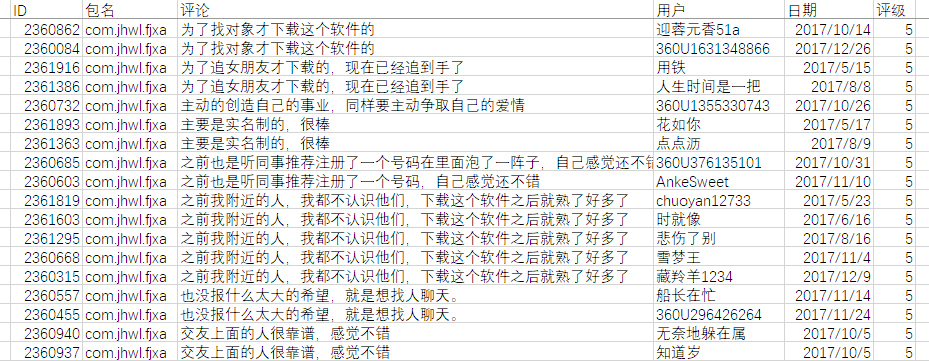
\includegraphics[width=\textwidth]{./Figures/edwin-cmt-sample-1.jpg}}\hfill

	\subfloat[\emph{com.arsenal.FunWeather}部分评论\label{fig:cmt-sample-2}]{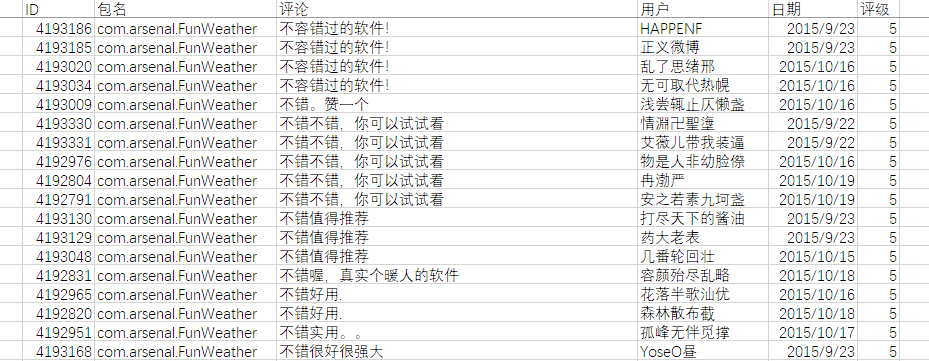
\includegraphics[width=\textwidth]{./Figures/edwin-cmt-sample-2.jpg}}\hfill

	\subfloat[\emph{com.sscwap}部分评论\label{fig:cmt-sample-3}]{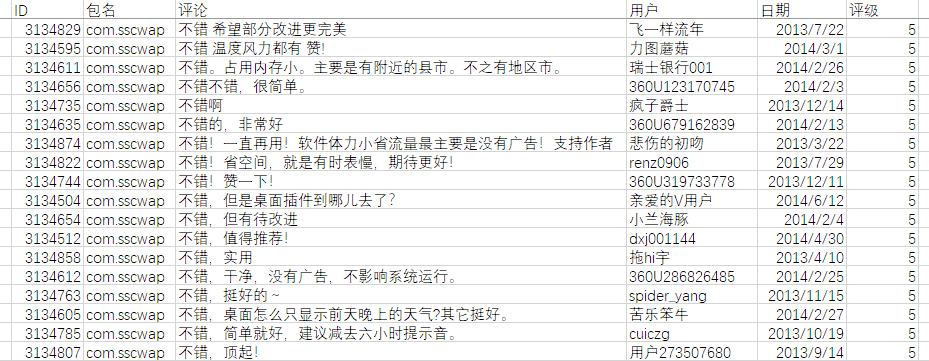
\includegraphics[width=\textwidth]{./Figures/edwin-cmt-sample-3.jpg}}\hfill
    \caption{应用评论取样}
    \label{fig:cmt-samples-1}
\end{figure}

\autoref{fig:cmt-samples-1}展示了本文对三款应用好评取样的结果。
可以明显看出,\emph{com.jhwl.fjxa}和\emph{com.arsenal.FunWeather}两款App都有明显的评论重复现象。
而图中对\emph{com.sscwap}的评论虽然看上去也比较近似,但这其实是由于本文按照评论内容对这些评论进行了一次排序。
如果结合日期数据观察,就能发现这些数据是由用户在比较分散的时间发出的。
所以说这些看上去稍微类似的评论,并不一定存在关联关系,笔者不倾向于认为这款App购买了排名欺诈服务。
反观\autoref{fig:cmt-sample-1}中的评论,有多条长评论高度相似、甚至一模一样,这在真实案例中是不太可能会存在的情况;而\autoref{fig:cmt-sample-2}中多条近似、相同的评论是在十分接近的时间里被发表的,进一步加深了他们之间存在关联的可能性,所以本文十分有理由相信这两款应用的确存在排名欺诈的行为。

本研究还随机抽取了一些发布相同好评的不同用户进行追查,结果发现部分用户在研究收集到的数据集中的评论数只有一到两条,这很有可能是提供排名欺诈服务的商家规避检测的一种策略。

\section{本章小结}
本章从仿冒应用在市场中收到的评论入手,首先分析了用户对于这类应用的反响。
用户给出的反馈为一致好评,这十分出人意料。
进一步地,为验证仿冒应用与排名欺诈是否有关联,本文选取了部分应用的评论数据进行分析,并借鉴了前人研究提出了研究手段进行筛查。

一方面,从结果看,无论是基于评论内容相似度的排名欺诈排查方法还是基于用户可信度权重的排查方法,都证明了仿冒应用的确会利用排名欺诈服务提升自身的曝光率。
另一方面,用两种方法进行筛查也顺便比较了他们的有效性。
从性能层面看,两种方法有较大的区别。
研究发现,部分可疑好评的用户仅仅评论过一到两次,如果大部分排名欺诈用户都采用这种只发布少量好评的策略,基于用户可信度权重的排查方法就很可能会因为可参考的数据量太小而失效;
另外,基于用户可信度权重的排查方法会带来相当大的运算量,相比之下,基于评论内容相似度的代码只需几分钟就能运算完毕。
综合上述因素,本研究认为基于评论内容相似度的排查方法是更为可行的排查方式。

\clearPaperPage

\chapter{总结与展望}
\label{chp:future}

\section{总结}
% In this paper we first introduce the concept of fake apps, and study specifically towards these apps.
在本文中,``仿冒应用''这个概念被率先引入。
然后,本文对这一方面进行了专门的研究,还搜集了大量的相关样本以辅助调查。
% To the best of our knowledge, we are the first to conduct a comprehensive empirical study on a large-scale fake apps.
本文的前期调研结果显示,本课题是第一个针对仿冒应用进行大规模全面实证研究的课题。

% To better understand the ecosystem nature of this type of apps, we obtained more than 150,000 data entries from real-world markets, observed and measured the fake samples among this dataset from several dimensions including certificate information, app size, app name and package name, time factor and so on.
为了更好地了解这个类型的应用的生态环境,本文基于Python 3设计实现了仿冒应用收集框架\mytool,利用基于BFS的算法收集了来自现实世界中各个应用市场的近14万个应用样本,并且从多个不同维度,对这个数据库里面的仿冒样本进行了观测和考察。
这些维度包括了APK包中的安全证书信息、应用大小、应用名、包名和时间因素等等。

% Through our measurements we gain valuable experience on fake apps from several perspectives, findings like fake samples' naming tendency and fake developers' evasive strategies are inferred.
然后,本工作将收集到的数据分为了\emph{仿冒应用的基本特征}、\emph{影响仿冒应用数量的因素}和\emph{仿冒应用的发展轨迹}三个不同视角进行了测量,获得如仿冒应用的命名倾向和仿冒应用开发者对市场监管防御机制的规避策略等信息。
% To support our findings, we further present a few study cases which provide us a more detailed look into fake apps to back our discoveries on fake app ecosystem.
为了佐证本文的发现,本研究在每个视角解读之后给出了从数据集中挑选的几个研究案例,呈现了如仿冒应用开发者对不同热门应用的仿冒方式的内容。
这几个案例进一步深化了本文对仿冒应用生态系统的发现。

之后,本文还收集了部分仿冒样本在商场上对应的评论和评级,排查仿冒应用是否利用了排名欺诈。
由于现有的排名欺诈检测手段尚有不足,本工作创新性地分别利用两种创新的研究方法---基于用户行为的用户可信度验证和基于NLP的评论内容相似度验证,对数据中的排名欺诈行为进行了排查。
结果显示,刷好评的排名欺诈行为的确存在于应用市场中,在本工作搜集到的仿冒应用评论中就有刷好评的痕迹。


\section{展望}

在大规模分析的部分中,本文中用到了三个不同的角度分别探索仿冒应用的特征,但回顾探索过程,一些方法和步骤依然不够深入。
如果能从以下三个角度再向仿冒应用入手研究,或许能有更多有所裨益的发现:

\begin{itemize}
    \item 应用图标:
    本文在进行案例研究中发现,不少仿冒应用的图标和原版官方应用的图标其实十分相像。
    因此,图标也可以是一个用于发掘/鉴别仿冒应用的突破口,研究者也许可以从应用图标中挖掘到更多可用的信息与行为模式。
    碍于时间因素所限,本文研究中并未加入图像对比处理部分提取各APK包中的图标与官方应用的图标进行比对,但如果能研究出快速比对多个应用间图标、图像相似度的算法,定当对应用市场的安全监管筛选机制有所好处。

    \item 应用内代码/文本/链接/ip分析:
    代码分析可以有效地剖析应用的行为,而相似的文本资源、链接等信息也可以提供各个App之间可能存在的关联关系。
    遗憾的是,从当前技术水平出发,仔细地对一个App进行完整而全面的静态分析所需时长太长,而动态分析需要测试样例驱动,自动化的动态测试工具往往未能深入拓展一个应用的大部分核心功能。
    因此,开发出快速的分析算法对App进行更深入的探索,就能挖掘出有关仿冒应用生态的更多信息。

    \item 仿冒应用总量的变化原因:
    \fullref{chp:discoveries}中提及到了Janus收集到的仿冒应用数量并非一直保持上升趋势。
    近年来,能搜集到的仿冒应用数量有突然下跌、甚至渐渐式微的迹象。
    究竟是什么因素导致了这个原因?是移动黑灰产内部的变化,还是安全厂商日益紧密的封锁?
    这将会是一个十分有趣的课题。
\end{itemize}

而在评论分析的部分中,也有可以继续发掘的部分。
在现阶段,学界关于排名欺诈的研究一直在针对积极评价方面,但是对应用差评进行排名欺诈的相关研究却有待补充。
刷好评可以提高应用评价提升应用排名,如果反其道而行之,用差评对目标应用进行攻击,其实也可以降低目标应用的评价,对其排名进行打击。
另外,在实际上,用户给的差评中含有相当多的有用信息。
用户对应用的不满、功能上的建议、bug的反馈,都可以反映在差评上。
关于用户差评,还有很多的研究空间。

最后,\mytool 框架本身,无论是代码层面还是设计层面,也有值得改善的地方。
比如是否能结合自动化爬虫框架提高爬虫模块的鲁棒性(对抗应用商店的反爬虫技术、下载稳定性),工具本身的代码优化,还有工具整体的易用性、稳定性等。

总之,从整体上看,本文的工作还有很多可以深化的部分。
然而,诚希望本文研究的结果能够为移动安全产业的从业人员(不论是工业界或学术界)提供足够的信息,以改善移动安全界的现状;或是抛砖引玉,在让读者对移动应用黑色产业有更多认识的同时,激发读者对仿冒应用等方面的研究兴趣,并从上述几点出发,为后人带来更多深入而完善的相关研究。

\clearPaperPage

% 参考文献
% 前置\cleardoublepage\phantomsection 以确保目录超链接到正确页码
\phantomsection\addcontentsline{toc}{chapter}{\small{参考文献}}
\bibliographystyle{GBT7714-2005}
\bibliography{bib/REFERENCE}
\clearPaperPage

% 攻读学位期间发表的学术论文
\fancypagestyle{plain}{%
	\fancyhead[LE,RO]{\small{\articleCategory}}
	\fancyhead[RE,LO]{\small{攻读学位期间发表的学术论文}}
}

\fancypagestyle{plain}{%
	\fancyhead[LE,RO]{华东师范大学硕士专业学位论文}
	\fancyhead[RE,LO]{ 攻读学位期间发表的学术论文}
}



\chapter*{攻读学位期间发表的学术论文}


\addcontentsline{toc}{chapter}{攻读学位期间发表的学术论文}


%\vskip 5mm

%{\heiti $\blacksquare$ 已公开发表论文}\vskip 5mm

\begin{enumerate}
	
	\item Chongbin Tang, Sen Chen, Lingling Fan, Lihua Xu, Yang Liu, Zhushou Tang, and Liang Dou, ``A large-scale empirical study on industrial fake apps,'' in \textit{Proceedings of the 41st International Conference on Software Engineering: Software Engineering in Practice,} IEEE Press, 2019: 183-192. (发表于CCF A类推荐学术会议, 软件工程方向顶级会议ICSE2019)
	
\end{enumerate}



\clearPaperPage

\fancypagestyle{plain}{%
	\fancyhead[LE,RO]{\small{\articleCategory}}
	\fancyhead[RE,LO]{\small{致\quad 谢}}
}
% 致谢。匿名与非匿名用不同版本
\ifx\anonymous \undefined
	\chapter*{ 致\qquad 谢}

\addcontentsline{toc}{chapter}{致  谢}




\vspace{0.2cm} \hspace{11.5cm}

\hspace{10.6cm}  二〇二〇年五月

\else
    \chapter*{ 致\qquad 谢}

\addcontentsline{toc}{chapter}{致  谢}

在师大的七年时光转瞬而逝,不知不觉,研究生历程已快要告一段落,我也将迎来下一个人生阶段。

借此机会,想对在师大遇上的各位老师和同学表示最真诚的感谢,尤其是我的导师,在我研究生的各个阶段都给予我鼓励和指导。同样想感谢的还有家里人和身边的朋友,是他们的支持帮助我走过了一路上的各种波折。


\vspace{0.2cm} \hspace{11.5cm}

\hspace{10.6cm}  二〇二〇年三月

\fi
\clearPaperPage


\end{document}
